\documentclass[12pt, oneside]{extbook}
\usepackage[utf8]{inputenc}
\usepackage{amsmath}
\usepackage{graphicx}
\usepackage{amssymb}
\usepackage{geometry}

\geometry{
	a4paper,
	top = 1.5cm,
	bottom = 1.5cm,
	left = 1.5cm,
	right = 1.5cm,
}

\author{Pierciro Caliandro}
\title{Sistemi Embedded e Real Time}

\begin{document}
\maketitle
\tableofcontents
\chapter{Introduzione ai Sistemi Embedded}
\section{Introduzione generale}
Un sistema embedded è un sistema programmabile, non pensato per essere riprogrammato dall'utente, è un'applicazione specializzata. Inoltre, i sistemi embedded sono fortemente immersi nell'ambiente circostante, ci sono sensori per interagire con l'utente. L'UI è invisibile o comunque non usuale (formata ad esempio da led o LCD), sono inoltre sistemi pervasivi, quindi non vengono notati.\\ Un sistema embedded è quindi una struttura di supporto al funzionamento di un applicazione, presentando come caratteristiche:
\begin{itemize}
\item un significativo livello di interazione con l'esterno
\item comandi o modalità operative che non sono selezionati direttamente da un operatore "umano"
\item sono calcolatori elettronici con un loro software, quindi vanno programmati
\end{itemize}
La diffusione dei sistemi embedded è vasta:
\begin{itemize}
\item Decine di microprocessori secondari del PC
\item Tastiere
\item Monitor LCD che hanno processori specializzati
\item Telefoni cellulari
\item Orologi
\item USB
\item ...
\end{itemize}
Tra il 98\% ed il 99\% dei dispositivi programmabili sono sistemi embedded, i campi di applicazione sono molteplici e spaziano dall'automotive, avionica, automazione industriale, telecomunicazioni agli apparati medicali, domotica, etc...\\ Ad esempio, in un auto a guida autonoma ci sono centinaia di sistemi embedded, collegati fra loro, che svolgono diverse funzionalità, composi da milioni di righe di codice. Questo comporta l'esposizione di una grande superficie di attacco che va quindi mantenuta sicura.
\subsection{Caratteristiche dei sistemi embedded}
A differenza dei moderni calcolatori elettronici, che sono dotati di un hardware molto potente e vario (molta memoria, molte CPU etc...), i sistemi embedded vengono sviluppati per eseguire un singolo compito e sono quindi ottimizzati seguendo particolari criteri.\\ Le tipiche funzionalità di un sistema embedded prevedono:
\begin{itemize}
\item Elaborazione: capacità di elaborare dati del mondo esterno, necessita di una determinata potenza di calcolo.
\item Comunicazione: capacità di trasmettere segnali da/verso il mondo esterno e dall'interno del sistema embedded
\item Memorizzazione: quante informazioni devo salvare nel tempo all'interno del sistema embedded
\end{itemize}
Ogni sistema embedded ha una storia a se, e vanno considerati alcuni parametri:
\begin{itemize}
\item Costo finale: un parametro importante, bisogna valutare bene dove viene integrato il sistema ed il suo costo.
\item Time to market: c'è l'esigenza per la progettazione di un nuovo sistema embedded, quindi non si può sforare
\item Tempo di vita: Può variare a seconda del sistema
\item Volume: Quanti pezzi del sistema penso di produrre
\item Interfacce di comunicazione: solitamente dal costo basso, ma comunque incidente
\item Interfacce utente: qualche pulsante e/o led, ad esempio uno schermo LCD
\item Consumo energetico: fattore cruciale, legato agli altri
\end{itemize}
Anche le capacità devono essere ben rapportate alle specifiche del sistema embedded:
\begin{itemize}
\item Dimensione del codice: il software deve essere bilanciato
\item Quality of Service: molte applicazioni hanno dei requisiti stringenti in termini di QoS, ad esempio i servizi in tempo reale (limiti temporali)
\item Aggiornamento del software: è utile includere questa capacità, il produttore permette l'aggiornamento senza ritirare il prodotto, questo permettere di risolvere eventuali guasti.
\item Affidabilità: valutazione realistica della probabilità di guasto
\item Manutenibilità: Probabilità di poter risparmiare in un certo tempo il sistema
\item Disponibilità: Probabilità che il sistema funzioni in ogni momento, vogliamo che abbia un valore alto
\item Safety: proprietà legata al fatto che un uso incorretto o un guasto provochi danni a cose o persone
\item Sicurezza: capacità di resistere contro gli utilizzi non autorizzati o non pensati in fase di progettazione. 
\end{itemize}
\chapter{Introduzione ai Sistemi Real-Time}
\section{Introduzione generale}
Informalmente, un sistema real-time è un sistema che deve lavorare secondo dei vincoli temporali ben precisi. Il sistema riceve un input, calcola un corretto output e questo calcolo viene effettuato entro dei limiti temporali.\\ La maggior parte dei sistemi embedded è anche real-time e viceversa, quando si progetta un sistema embedded non si può tralasciare il sistema operativo e l'applicazione che vi verrà eseguita.\\ La tipologia del sistema operativo real-time è un fattore critico, in tutte le applicazioni safety-critical. La teoria della schedulazione real-time studia cosa è possibile ottenere avendo a disposizione un certo hardware, con potenza di calcolo limitata.\\ I sistemi embedded interagiscono con l'ambiente circostante, reagendo rapidamente ai segnali esterni. Ad esempio, un aribag attivato da un sistema embedded deve avvenire in tempi precisi, se avviene prima o dopo il tempo corretto, ci sono dei gravi rischi sulla salute del passeggero, quindi i limiti temporali devono essere estremamente precisi.\\ Non è possibile progettare l'hardware separatamente dal software, bisogna fin da subito stabilire il tipo di applicazione e di conseguenza il tipo di sistema real-time da porre sul sistema embedded. Anche nel caso di sistemi embedded bare metal, bisogna prima stabilire un'organizzazione iniziale, specialmente per sistemi safety-critical, in qual caso è necessario certificare il sistema.
\subsection{Teoria della schedulazione real-time}
Nella teoria della schedulazione real-time, ho una CPU con una certa potenza di calcolo, ci sono poi dei processi che svolgono dei task che hanno delle scadenze. L'obiettivo è avere un algoritmo di schedulazione che permetta di rispettare le scadenze. Si cerca di modellare il sistema reale in modo da far si che i task possano essere completati entro le scadenze temporali.\\ Ammettendo di avere una potenza di calcolo superiore, i tempi sarebbero ridotti, quindi sembrerebbe che la teoria della schedulazione non serva, ma in verità non è così: in alcuni casi infatti, aumentare la potenza di calcolo non aiuta, mentre il altri non è proprio possibile per motivi di budget.\\ Un altro problema da dover affrontare nei sistemi real-time riguarda la possibilità di eseguire test: questi infatti possono essere eseguiti, ma non sono sufficienti. Occorre quindi la certezza matematica che il sistema sia ben progettato.\\ I parametri temporali del sistema sono noti a priori, sono tipici dell'ambiente applicativo. Ad esempio, i sistemi di controllo digitale, che sono sistemi real-time impiegati in sensori ed adattatori come controllori: 
\begin{enumerate}
\item eseguono un loop infinito, in cui leggono un dato
\item il dato viene convertito da analogico a digitale
\item confrontando con lo stato l'obiettivo da raggiungere, mediante una legge di controllo, viene fornito l'output
\end{enumerate}
È un esempio di feedback control loop, posso avere sistemi a frequenza unica e sistemi multi frequenza.\\ Un altro esempio è il controllore di volo di un elicottero (1975-1980), in cui viene reiterato un ciclo ogni $\frac{1}{180}sec$ ed avvengono delle azioni: 
\begin{itemize}
\item[T1)] Convalida i dati dei sensori per selezionare quelli che vanno acquisiti, in caso di guasto riconfigura il sistema
\item[T2)] Esegue una delle funzioni avioniche, con la frequenza $30Hz$:
\begin{itemize}
\item[-] campiona i controlli del pilota
\item[-] esegue la normalizzazione dei dati e la trasformazione delle coordinate
\item[-] aggiorna la posizione del veicolo  
\end{itemize}
\item[T3)] In alternativa a T2, sempre a $30Hz$, esegua una delle funzioni di controllo (per le possibili posizioni dell'elicottero):
\begin{itemize}
\item[-] calcola la legge di controllo esterna del pitch
\item[-] calcola la legge esterna del rollio
\item[-] calcola la legge esterna di yaw e movimento
\end{itemize}
\item[T4)] Esegue una delle seguenti funzioni, a $90Hz$ di frequenza, usando i risultati di T2 e T3: 
\begin{itemize}
\item[-] Calcola la legge di controllo interna del pitch
\item[-] Calcola la legge interna di rollio  e movimento
\end{itemize}
\item[T5)] Eseguito con i risultati di T4, calcola la legge di controllo interna per lo yaw
\item[T6)] Fornisce l'output agli attuatori
\item[T7)] Effettua test interni per la consistenza
\end{itemize}
Il controllo di volo è una black box con un computer a capacità limitata, in $\frac{1}{180}sec$ il processore non riesce ad eseguire tutti i task, per questo vi è la distinzione fra leggi di controllo interne ed esterne: quelle interne sono delle approssimazioni della vera legge di controllo, che quindi hanno un certo errore, mentre le leggi esterne sono costituite da calcoli più pesanti ma senza errore.\\ A regime, ci sarà un certo errore ma occasionalmente verrà corretto, questo permette di avere una traiettoria di volo stabile.\\ Ci sono però dei vincoli real-time, ad esempio lo yaw è più pesante da calcolare perché la direzione è più complessa. Inoltre, non è possibile eseguire tutti i task in uno stesso ciclo, quindi è compito del progettista decidere cosa fare in quale ciclo.
\subsection{Esempi di sistemi real-time}
Vi sono diversi esempi di sistemi real-time che possono essere considerati:
\begin{itemize}
\item Sistemi di controllo ad alto livello: ad esempio una sala di terapia intensiva, in cui dei sistemi di controllo di basso livello manda i dati a quelli di livello alto, che li processano e li usano per tenere i parametri vitali stabili. C'è poi un sistema generale per mostrare il quadro clinico di ciascun letto, ed un altro che avverte se un paziente ha una crisi. Devono essere sistemi embedded real-time, gli avvisi ad esempio devono essere inviati entro un tempo limite
\item Processamento di segnali: sistemi radar, con un antenna che viene puntata in una certa direzione e manda impulso elettromagnetico, ascolta poi l'eco (se colpisce eventuali ostacoli). Se viene misurata la frequenza dell'eco, a causa dell'effetto doppler capisco la velocità relativa dell'oggetto rispetto a me, viene inoltre misurato il ritardo d'eco (la distanza); è importante filtrare il rumore.\\ Il radar ha un DB in cui contiene gli oggetti rilevati, è necessario capire se un oggetto è vecchio o nuovo, perché magari si è mosso e questo va fatto in tempi rapidi, prima che l'antenna rilevi la nuova posizione.
\item Basi di dati temporali: la validità dei dati è direttamente/inversamente proporzionale al momento in cui questo è stato inserito
\item Mercato finanziario: viene regolato da DB che memorizzano il valore dei titoli, che viene continuamente aggiornato, i dati vengono selezionati in base alla "freschezza" (da quanto tempo sono stati aggiornati).
\item Applicazioni multimediali: i flussi di dati vengono compressi con degli appositi algoritmi per poi venire decompressi. Queste operazioni vanno fatte in "tempi utili", o si rischierebbe di andare fuori sync.
\end{itemize}
\subsection{Nomenclatura nei sistemi real-time}
Un sistema effettua il mapping fra un valore di input ed il valore di output risultante. La correttezza logica risiede nel fatto che per un certo valore di input, verrà prodotto il corretto valore di output.\\ Un sistema real-time è un sistema la cui correttezza logica dipende non solo dal risultato fornito come output, ma anche dall'istante temporale in cui l'output è reso disponibile.\\ Un'applicazione real-time è un programma o insieme di programmi con vincoli temporali ben definiti, mentre un sistema real-time è un insieme di dispositivi hardware e software che rendono possibile la corretta esecuzione di un applicazione real-time.\\ I sistemi real-time si possono dividere in:
\begin{itemize}
\item sistemi puramente ciclici: ogni task è eseguito periodicamente, non esistono variazioni significative nell'uso di risorse nel tempo
\item sistemi per lo più ciclici: alcuni task vanno gestiti a parte, ad esempio quelli per la gestione degli errori
\item sistemi asincroni ma predicibili: non si sa quando eseguire un task, ma bene o male si riesce a stimare.
\item sistemi asincroni e non predicibili: non so se e quando arriva un task, ma quando arriva ci sono dei vincoli temporali ben precisi.
\end{itemize}
Un job è l'unità di lavoro minima che può essere schedulata ed eseguita da un sistema real-time, ad esempio 
\begin{itemize}
\item un processo
\item la spedizione di un messaggio su un canale di comunicazione
\item la lettura di un file da un dispositivo di massa 
\end{itemize}
Un task è un insieme di job tra loro correlati, che uniti realizzano una determinata funzione del sistema, ad esempio un task può essere formato dal:
\begin{itemize}
\item Job che acquisisce i dati di un sensore
\item Job che converte i valori in un formato appropriato
\item Job che aggiorna con i valori convertiti alcune strutture dati
\end{itemize}
In uno stesso task, un job non può iniziare se il job che lo precede nel task non è terminata.\\ Per processore, si intende una componente attiva del sistema real-time in grado di eseguire un job:
\begin{itemize}
\item CPU
\item Disco rigido
\item Canale di rete
\item ...
\end{itemize}
Il sistema real-time viene modellato astraendo dei particolari, quindi vengono tratte le conclusioni valide per più tipologie di sistemi, nel modello verranno tralasciati i dettagli.\\ Una risorsa è una componente del sistema la cui disponibilità è necessaria per eseguire determinati job. È una componente passiva: nel processore, c'è una dotazione intrinseca di velocità, più questo è rapido e maggiore sarà il numero di job che potrà eseguire.\\ La risorsa è un elemento in cui il fattore velocità non incide ad esempio:
\begin{itemize}
\item un semaforo System V
\item la memoria di un sistema
\item altre risorse, che dipendono dal problema in esame
\end{itemize}
L'istante di rilascio di un job è l'istante temporale in cui un job diviene disponibile per l'esecuzione.\\ La scadenza di un job è invece l'istante temporale entro cui il job deve aver finito l'esecuzione. Spesso è conveniente ragionare in termini di tempo di risposta del job, ovvero l'intervallo fra il suo rilascio e l'istante in cui completa l'esecuzione.\\ La scadenza relativa è il massimo tempo di risposta ammesso per un job, in particolare abbiamo che: scadenza (assoluta) = istante di rilascio + scadenza relativa.
\subsection{Sistemi hard e soft real-time}
Ci sono varie definizioni, ma tutte hanno dei problemi:
\begin{itemize}
\item Quanto è possibile tollerare i vincoli temporali di un job?
\item Quanto è utile completare un job dopo la sua deadline?
\item Quanto è statisticamente frequente violare i vincoli di un job?
\end{itemize}
Abbiamo che:
\begin{itemize}
\item un sistema hard real-time è un sistema in cui qualcosa che non rispetta i vincoli temporali provoca un danno fatale, con effetti disastrosi
\item un sistema soft real-time è un sistema in cui la mancanza di una deadline non ha effetti disastrosi
\end{itemize}
La definizione ha comunque dei limiti: il criterio con cui si definisce un "danno fatale, con effetti disastrosi", è soggettivo.\\ Un'altra definizione si basa sulla funzione di utilità dei job, ovvero quanto è utile completare quel job dopo la sua scadenza:
\begin{itemize}
\item in un sistema hard real-time, la funzione di utilità di un job si abbatte se il job è in ritardo
\item in un sistema soft real-time, invece, la funzione di utilità decresce gradualmente in funzione della tardività. La tardività di un job è il ritardo con cui il job completa la sua esecuzione rispetto alla scadenza
\end{itemize}
Nel caso di sistemi hard real-time, l'utilità si annulla o diventa negativa al crescere della tardività. Avere un utilità negativa vuol dire che il sistema trae vantaggio dal non completare il job in ritardo.\\ Anche qui, il limite sta nel modo in cui si assegna la funzione di utilità, che è arbitrario e frutto di opinioni personali.\\ Un'ultima definizione parla invece della violazione dei vincoli temporali:
\begin{itemize}
\item in un sistema hard rea-time, un job non deve mai violare un vincolo temporale
\item in un sistema soft real-time un job può sforare il vincolo in certe condizioni
\end{itemize}
In questo caso, il limite sta nel termine mai, che corrisponderebbe ad una probabilità dello 0\%, che non è reale.\\ La definizione operativa parla del vincolo temporale di un job:
\begin{itemize}
\item un vincolo temporale di un job è hard real-time (e di conseguenza anche il job) se è richiesta una validazione che tale vincolo temporale verrà sempre soddisfatto. La validazione è una dimostrazione matematica che in nessun caso possibile le sequenze dei job che si alternano possono fallire e mancare le scadenze; o anche un evidenza sperimentale prodotta da test esaustivi.
\item Un vincolo temporale di un job è soft real-time se non è richiesta una validazione, oppure se basta una dimostrazione che il job soddisfa il completamento entro dei limiti statistici.
\end{itemize}
La validazione va effettuata in fase di progettazione del sistema: si effettua l'analisi dei rischi, si pensa alla safety security, alle implicazioni in casi di guasti etc...\\ I rischi vengono classificati, il modello di riferimento per la valutazione è la gravità del fallimento.\\ I meccanismi per la riduzione dei rischi prevedono la definizione di vincoli temporali da rispettare, il rispetto dei vincoli temporali è la condizione per minimizzare i rischi e tale rispetto è tanto più importante quanto maggiore è la gravità del rischio.\\ La metrica non è universale e va realizzata in base alla tipologia di progetto.
\subsection{Modello di riferimento per sistemi real-time}
Occorre definire un modello per realizzare il sistema real-time, a partire da un modello teorico.\\ In  un sistema hard real-time non è possibile pensare di costruire un sistema che sia il più veloce possibile, l'unica considerazione che va effettuata è se tale sistema rispetta o meno i vincoli temporali definiti, qualunque cosa accada.\\ Non bisogna pensare di poter minimizzare i tempi di risposta, in quanto è un ragionamento che può avere valenza per un singolo task, ma per sistemi con molteplici task, questo introduce difficoltà al problema di far rispettare le scadenze.\\ La definizione operativa di sistema real-time prevede che venga prodotto un certificato sia nell'hardware che nel software. ad esempio, il certificatore può dire che il software deve rispettare le scadenze in modo deterministico, anche entro dei precisi limiti (caso pratico di sistemi in cui si parla di funzione di utilità dei job).\\ Un sistema soft real-time ha dei vincoli in cui il rispetto della scadenza temporale non è essenziale per validità del sistema, quindi è possibile ottimizzare altri parametri:
\begin{itemize}
\item throughtput
\item tempi di risposta
\item ...
\end{itemize} 
Ogni sistema real-time si può riassumere in 3 componenti:
\begin{itemize}
\item Modello del carico: l'applicazione che il sistema deve supportare
\item Modello delle risorse: risorse del sistema a disposizione dell'applicazione
\item Algoritmi: come il sistema distribuisce le risorse nel tempo
\end{itemize}
In questo modo è possibile catturare la complessità del sistema, è necessario anche includere tutti gli aspetti per la comprensione del sistema anche se in modo non dettagliato. Più il modello è semplice, più il risultato è applicabile in sistemi analoghi.\\ È possibile identificare 2 tipologie di risorse differenti:
\begin{itemize}
\item Risorse attive: anche dette server o processi (non per forza una CPU), canali di comunicazione, dischi rigidi etc...
\item Risorse passive: risorse come memorie, numeri di sequenza, primitive di sincronizzazione, ...
\end{itemize} 
Nel modellare un sistema, viene scritto l'elenco dei processi $p_1$, $p_2$,...,$p_m$ e le risorse passive $r_1$,..., $r_j$. Se la risorsa è così abbondante da non essere un problema, non ha senso metterla nel modello; se invece non è così allora ha senso modellarla.\\ I job all'interno del sistema si categorizzano in base ai vincoli temporali, ai parametri funzionali, alla dipendenza da altri job del sistema.\\ Le istanze di rilascio dei job si indicano con $r_i$ per il job i-esimo, mentre la deadline è indicata con $d_i$. La scadenza relativa $D_i$ = $d_i - r_i$, è invece il tempo massimo che può intercorrere tra l'istante di rilascio del job ed il suo completamento.\\ L'intervallo di fattibilità è indicato con ($r_i$, $d_i$], i vincoli temporali sono specifiche del sistema real-time di riferimento, possono anche essere intervalli, ad esempio $r_i \in [r_i^{-}, r_i^{+}]$.\\ Molti sistemi real-time sono di tipo periodico, ma nel sistema deve essere possibile poter gestire i task in tempi casuali: job che arrivano in istanti casuali rendono problematico la pre-riservatezza delle risorse.\\ Altre tipologie possibili di task sono:
\begin{itemize}
\item Task aperiodici: in cui gli istanti di rilascio dei job sono casuali e non predefiniti
\item Task sporadici: Gli istanti di rilascio dei job sono casuali, ma esiste un intervallo di tempo minimo tra il rilascio di due job
\end{itemize}
Il tempo di esecuzione $e_i$ di un job $J_i$ è l'ammontare di tempo necessario per il completamento quando sono disponibili tutte le risorse necessarie, quindi come se eseguisse isolato.\\ Tale valore non dipende dal tipo di scheduling, ma da ciò che il job deve fare e dalle caratteristiche del processore.\\ Tutti i processori moderni hanno un comportamento non deterministico, non è possibile prevedere il tempo di esecuzione dei job in quanto questo dipende dallo stato interno del processore stesso e tale stato dipende a sua volta dalla sequenza di istruzioni che lo hanno portato in quello stato.\\ Il tempo varia da esecuzione ad esecuzione, quindi è possibile solamente individuare un intervallo: $e_i \in [e_i^{-}, e_i^{+}]$.\\ Per rispettare le scadenze conta il worst case: se il risultato è pronto in anticipo, è possibile far attendere il job , ma se invece arriva in ritardo questo è un problema. Conoscere il tempo massimo di un job è sufficiente per capire se il sistema rispetterà o meno le scadenze. Indichiamo il tempo massimo con $e_i^{+}$ o wcet (worst case execution time), quindi da adesso in poi con tempo di esecuzione intenderemo il wcet.\\ In sistemi hard real-time, essendo necessaria una certificazione, bisogna conoscere i tempi di esecuzione dei job hard (il wcet può cambiare anche in caso di job isolato). Una proprietà importante è la predicibilità, ovvero il numero di di test su un job che portano a dei wcet vicini fra loro.\\ Per poter aumentare la predicibilità, è necessario semplificare il sistema: si sceglie un hardware meno sofisticato, si evitano interazioni complesse fra i job, l'uso di strutture dati dinamiche e di troppe primitive di sincronizzazione.
\subsubsection{Modello di carico deterministico a task periodici}
È un modello che rappresenta bene molti sistemi real-time, gli algoritmi di scheduling usati sono semplici ed efficienti, vi è la teoria matematica per la certificazione anche se presenta dei limiti. Non è ad esempio possibile rappresentare bene job che hanno dei jitter alti per gli istanti di rilascio o un alta varianza di $e_i$.\\ Il principio base è che ogni attività che si esegue a cadenza regolare è un task periodico.\\ Un task $T_i$ è una sequenza di job, il periodo $p_i$ è l'intervallo temporale tra gli istanti di rilascio dei job di $T_i$ ed il tempo di esecuzione è il massimo fra tutti i tempi di esecuzione $e_i$ dei job $J_i$ di $T_i$.\\ Avendo n task $T_1$, $T_2$,...,$T_n$, indichiamo i job del task $T_i$ = $J_{i,1}$, $J_{i,2}$,...,$J_{i,n}$, con $J_1$,..,$J_n$ indichiamo i job di sistema.\\ $r_{i,1}$ è l'istante di rilascio del job $J_{i,1}$ di $T_i$ e $\phi_i$ è la sua fase. Task che hanno la stessa $\phi$ sono detti in fase. Indichiamo con H il minimo comune multiplo dei periodi $p_i$ dei task $T_i$ del sistema. Un iper-periodo è un intervallo di lunghezza H di task periodici. N è il numero massimo di job in ogni iper-periodo ed è pari a $N = \sum\limits_{i=1}^{n} \frac{H}{p_i}$. L'utilizzazione $u_i$ del task $T_i$ è pari ad $u_i = \frac{e_i}{p_i}$, dove $e_i$ è il tempo di esecuzione del task $T_i$ e $p_i$ il suo periodo.\\ Se $T_i$ ha una utilizzazione pari ad 1, vuol dire che il task occupa il processore per un tempo pari alla lunghezza del periodo. Non appena il job finisce, viene rilasciato un secondo job e così via: l'impatto è la saturazione di un processo.\\ L'utilizzazione totale del sistema è $U = \sum\limits_{i=1}^{n} u_i$. Tutti i job di uno stesso task hanno la stessa scadenza relativa $D_i$, se un job è rilasciato all'istante t va completato entro $t + D_i$. In molti casi un sistema real-time può essere modellato assumendo che tutti i job abbiano istante di rilascio coincidente con l'inizio di ciascun periodo e scadenze implicite, ossia $D_i = p_i$.\\ esempio: $p_1 = 3$, $p_2 = 4$, $p_3 = 10$, 3 task tutti in fase, $e_1 = 1$, $e_1 = 1$, $e_1 = 3$. Quanti sono i differenti job del sistema? Non è possibile dirlo, ma non importa: posso sapere quanti ce ne sono in un iper-periodo: H = mcm(3,4,10) = 60  N = $\sum\limits_{i=1}^{3} \frac{H}{p_i}$ = 41.\\ È importante capire quanti job ogni task rilascia in un iper-periodo: 60 è il primo istante in cui tutti i periodi dei task tornano ad essere in fase. L'utilizzazione totale è data da $u_1$ + $u_2$ + $u_3$ = $\frac{53}{60} \approx 88.3\%$. È possibile schedulare i task con un solo processore se le scadenze son implicite? Posso eseguire un job alla volta e riesco a schedularli in modo che un job finisca prima che prima che inizi il successivo. Ci saranno degli intervalli vuoti nell'iper-periodo, ma questo era noto visto che la U è $<$ 1.\\ Un vincolo di precedenza è una condizione che impone di schedulare due job J e J' in un ordine preciso. È una relazione d'ordine parziale fra job: $J \prec J'$ se $J'$ deve attendere l'esecuzione di J. Se i vincoli di precedenza sono totali c'è una semplificazione nello scheduling dei task.\\ È possibile rappresentare le precedenze con un grafo diretto aciclico, dove gli archi sono le precedenze immediate fra job.\\ I parametri funzionali di un job sono:
\begin{itemize}
\item interrompibilità del job: è possibile interrompere l'esecuzione di un job per poi continuarla
\item criticalità
\item funzione di utilizzazione
\end{itemize}
Un job è interrompibile se la sua esecuzione può essere sospesa in qualunque istante per dare spazio ad altri job, per poi essere ripresa.\\ Non esistono job sempre interrompibili in quanto le condizioni possono far si che il job non lo sia. Ad esempio nella programmazione di un dispositivo hardware, la modifica di una struttura dati condivisa con altri job richiede il salvataggio delle informazioni che permettono di riprendere l'esecuzione.\\ Tale insieme di informazioni, che occorrono per riprendere l'esecuzione a seguito di un interruzione, è chiamato contesto.\\ Un cambio di contesto è una procedura con la quale si salva il contesto di un job e si recupera il contesto del job che prende il suo posto in esecuzione.\\ Il tempo per effettuare il context switch è un parametro cruciale, in quanto toglie tempo al processore e quindi all'esecuzione del job.\\ La criticalità di un job è la sua importanza rispetto agli altri job del sistema, non va confusa con la priorità o il peso, che sono attributi non necessariamente legati alla criticalità.\\ La funzione di utilità di un job va distinta in base al tipo di job (se hard o soft real-time) ed indica quanto è utile completare un job se questo è in ritardo.\\ È un parametro soggettivo, quindi non va considerato come parametro di sistema.\\
\begin{figure}[!h]
\centering
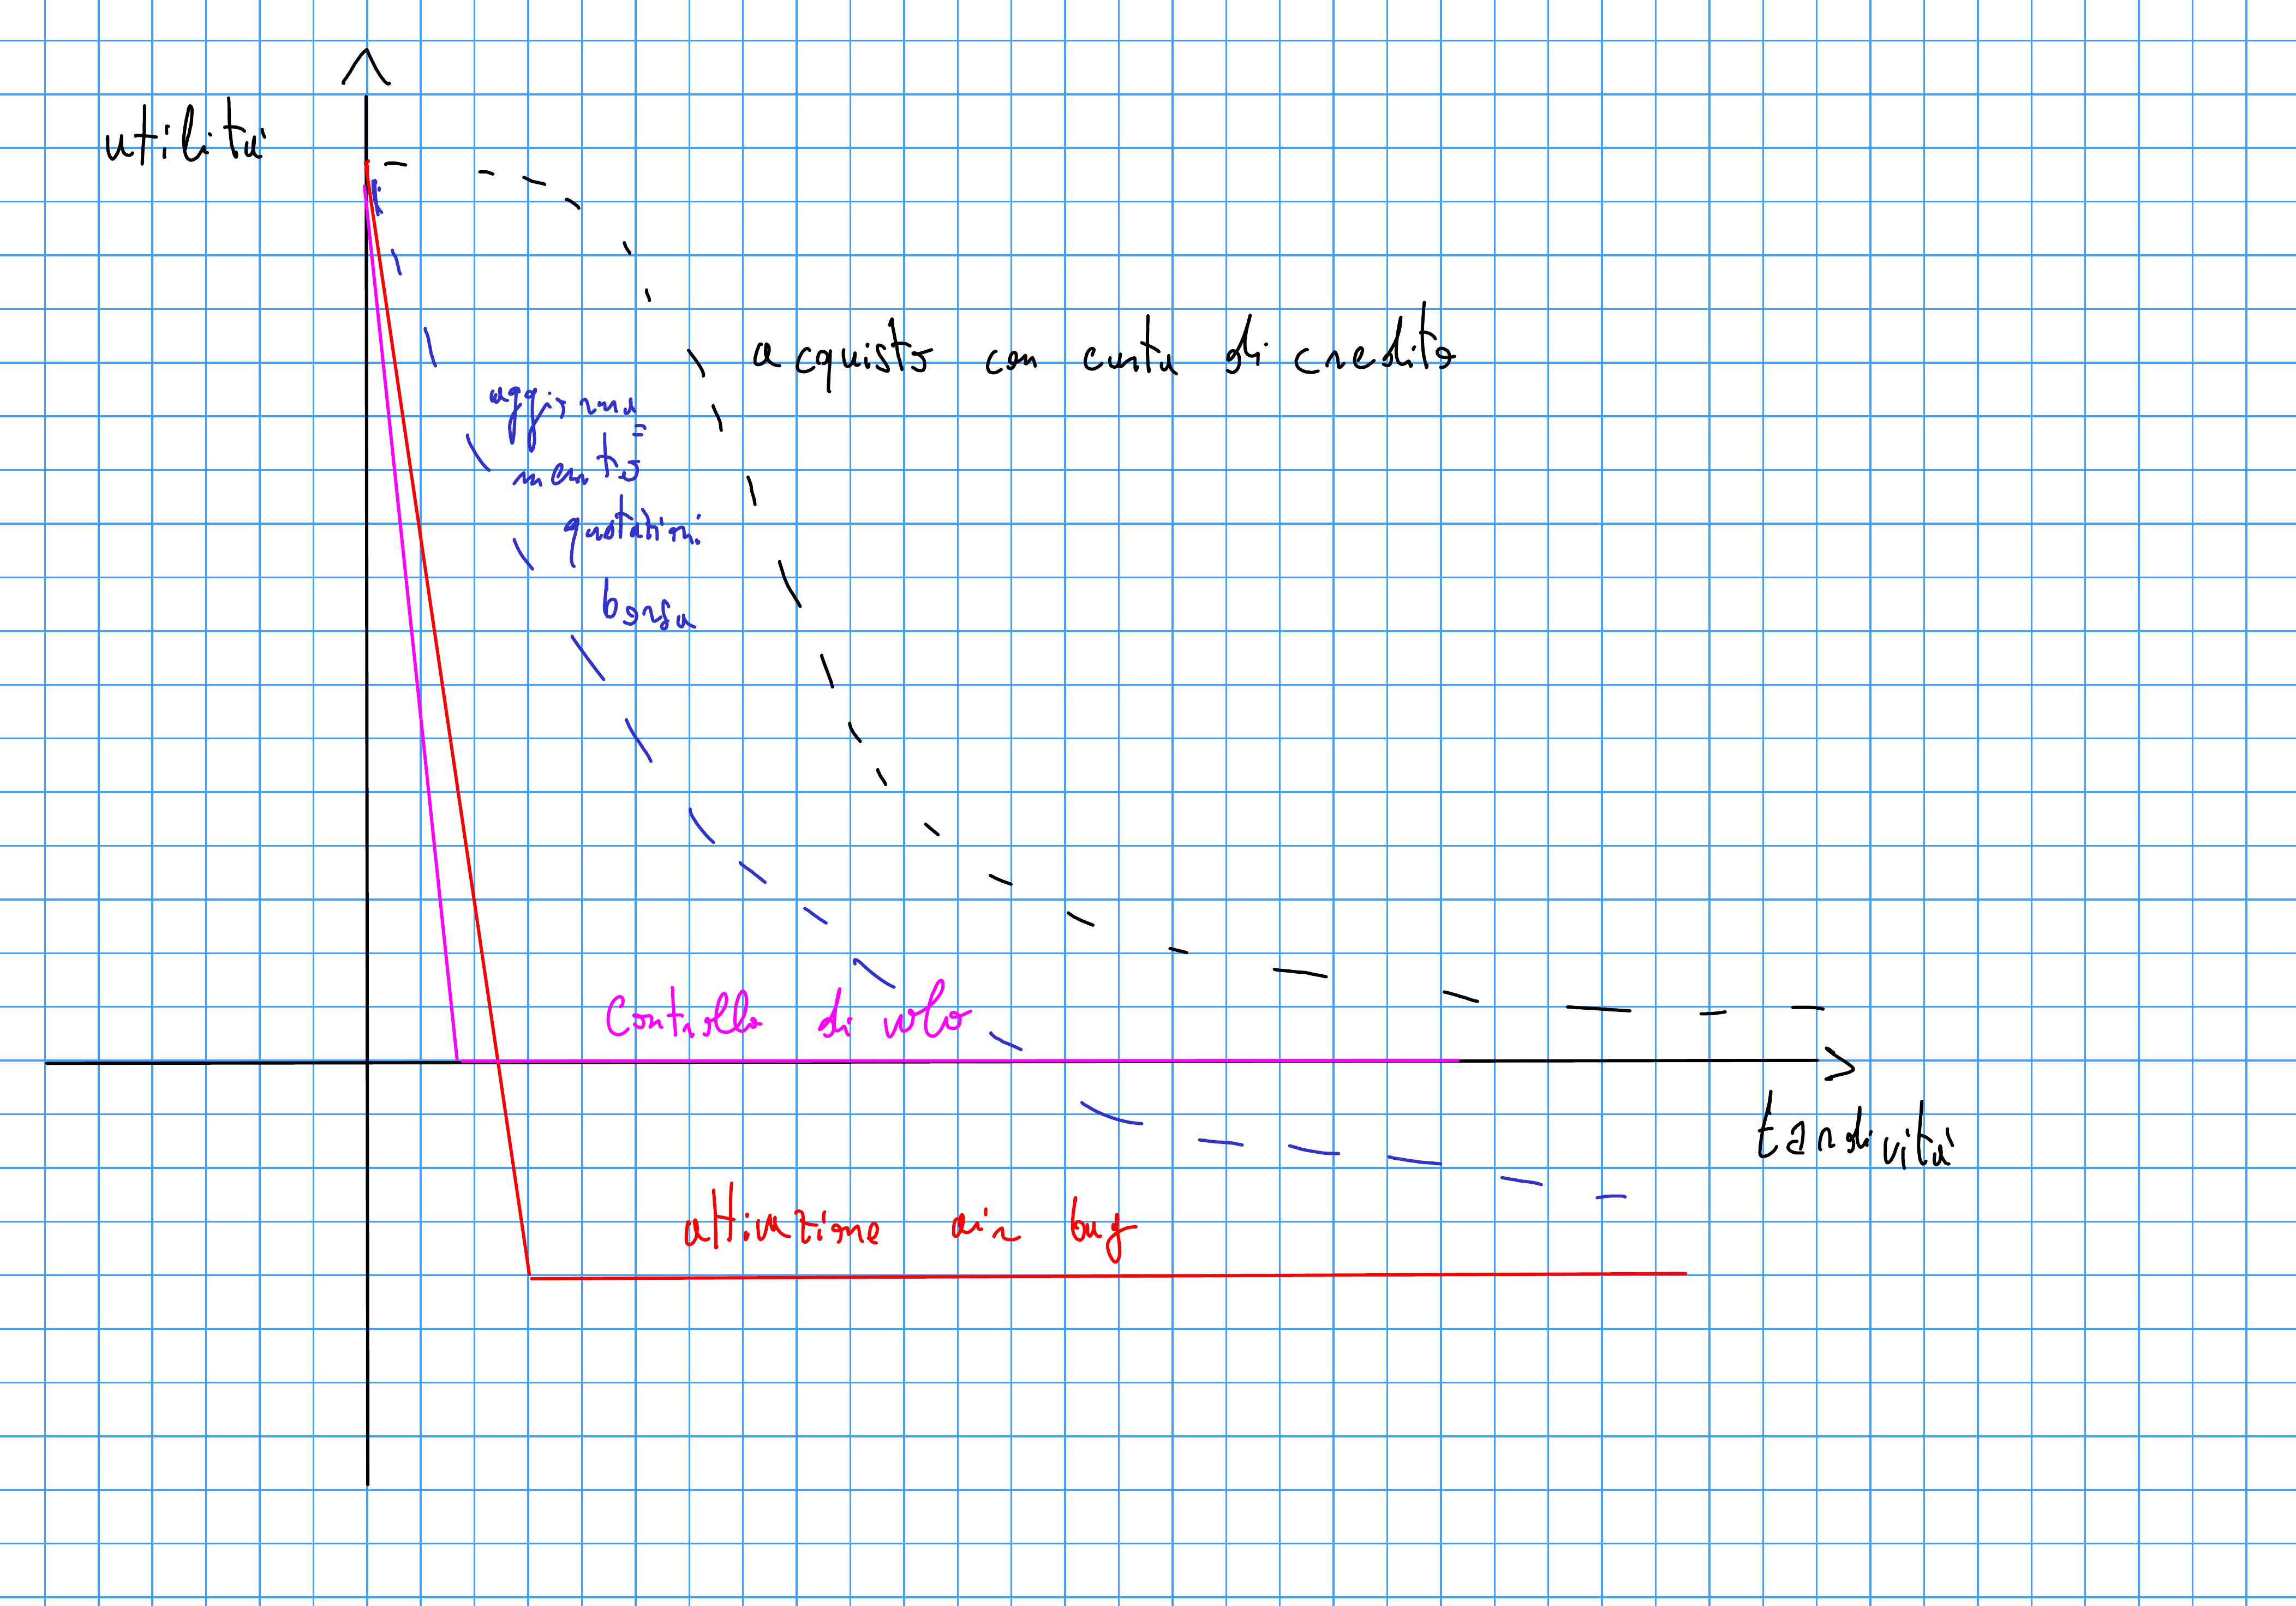
\includegraphics[scale=0.4]{immagini/image-000.jpg}
\end{figure}
\subsection{Scheduler}
Uno scheduler è un modulo del sistema che utilizza un algoritmo per ordinare l'esecuzione e l'accesso alle risorse. Uno schedule è l'assegnazione dei job ai processi disponibili, una schedulazione si dice valida se:
\begin{itemize}
\item ogni processore esegue al più un job in un certo momento
\item in ogni istante un job è assegnato al più ad un processore
\item se un job viene rilasciato in un certo istante non può essere eseguito prima di tale istante
\item un job non può essere assegnato per più del suo tempo di esecuzione
\item tutti i vincoli di precedenza e di uso delle risorse fra i job sono rispettati
\end{itemize}
Una schedulazione è valida e fattibile se ongi job viene completato entro la sua scadenza, un insieme di job si dice schedulabile da un algoritmo di schedulazione se questo produce sempre una schedulazione fattibile per quell'insieme.\\ Un algoritmo è detto ottimale se produce sempre una schedulazione fattibile quando l'insieme dei job è schedulabile. Per valutare un sistema real-time è possibile misurare le prestazioni:
\begin{itemize}
\item Tardività: pari a 0 se le scadenze vengono rispettate o è pari alla differenza fra completamento e scadenza
\item Lateness: differenza fra l'istante di completamento e la scadenza. È negativa se viene rispettata la deadline, tanto più è piccola e tanto più si completa lontano dalla scadenza. Occorre rendere il sistema predicibile, quindi tentare di completare vicini alle scadenze, consideriamo le seguenti quantità:
\begin{itemize}
\item tempo di risposta: $istante di completamento - istante di rilascio$
\item miss rate: \% dei job che completano oltre la scadenza
\item loss rate: \% dei job soft real-time non eseguiti o non terminati
\item  invalid rate: $miss rate + loss rate$
\end{itemize}
\end{itemize}
\subsubsection{Scheduler clock-driven e priority-driven}
Esistono vari tipi di algoritmi di scehdulazione, un algoritmo clock driven prende delle decisioni solo limitate al controllo di quali job effettivamente sono disponibili per l'esecuzione.\\ È il progettista del sistema a dover decidere la schedulazione, o scheduler si limiterà a controllare se i job sono stati rilasciati.\\ Le decisioni verranno prese in intervalli di tempo ben definiti: il tempo infatti, verrà diviso in intervalli ed in tempi fissati lo scheduler controllerà se i job da eseguire sono presenti, altrimenti passerà ai prossimi (seguendo l'ordine definito dal progettista). È necessario conoscere i task con i rispettivi parametri funzionali, inoltre la schedulazione risultante è costruita a priori (off-line) dal progettista.\\ Lo scheduler deve intervenire ad intervalli di tempo ben definiti, usando dei componenti hardware detti clock o timer, che scandiscono i tempi in cui lo scheduler deve intervenire.\\ I vantaggi di tale approccio sono molteplici:
\begin{itemize}
\item semplicità
\item efficienza, in quanto l'overhead è minimo
\item facilità nel validare il sistema nel caso sia hard real-time
\end{itemize}
Come svantaggio c'è sicuramente la mancanza di flessibilità, in quanto non è possibile gestire task che non sono previsti in fase di progetto, oppure nuovi task a run-time.\\ La tendenza attuale è quella di usare scheduler priority-driven, che sono più flessibili. Infatti, scheduler clock-driven prevedono che la decisione sia prefissata e che venga presa in intervalli di tempo precisi. Sono quindi adatti a sistemi deterministici, in cui i parametri dei job sono fissati ed in cui è possibile calcolare una volta e per tutte la schedulazione. Se ci sono task periodici, la schedulazione prodotta sarà ciclica.\\ Nel caso di algoritmi priority-driven, ad ogni invocazione dello scheduler questo ha un comportamento dinamico e reagisce agli eventi; si parla quindi di sistemi on-line con algoritmi dinamici.
\subsubsection{Schedulazione ciclica e statica}
Si ragiona su un modello a task periodici:
\begin{itemize}
\item il numero di task è prefissato, pari ad n
\item i parametri dei task sono prefissati
\item ogni job può essere eseguito dal suo istante di rilascio (nessun vincolo o conflitto sulle risorse)
\item possono esistere job aperiodici con vincoli temporali soft o hard real-time
\end{itemize}
Nel caso in cui si indica la tripla ($p_i, e_i, D_i$) è implicito che la fase sia pari a 0, mentre per la coppia ($p_i, e_i$) si ha $D_i$ = $p_i$.\\ esempio: $T_1$= (4, 1), $T_2$= (5, 1.8), $T_3$= (20, 2), singolo processore. Derivare una schedulazione fattibile.\\ H = mcm(4, 5, 20) = 20, cerco una schedulazione fattibile in H, ma tenendo in considerazione le fasi $\phi_i$, in questo caso tutte pari a 0 $\forall i$. Se riesco a ricavare una schedulazione fattibile, la ripeto all'infinito.\\ L'implementazione per derivare la schedulazione prevede la costruzione di una tabella: indico con $t_k$ l'istante in cui una decisione viene presa, T($t_k$) sarà il nome del job o del task da eseguire all'istante $t_k$, se il processore sarà idle lo indicherò con I.\\I job aperiodici soft real-time saranno schedulati negli intervalli I, ma verranno interrotti se non completati entro il $t_k$ successivo (nel caso in cui arrivi un job periodico).\\ In questa prima versione non prevediamo job aperiodici hard real-time. Uno scheduler di questo tipo è anche detto scheduler a tabella, è conveniente però avere degli scheduler più sofisticati con determinate proprietà:
\begin{itemize}
\item l'attivazione dello scheduler avviene ad intervalli regolari
\item la distribuzione degli intervalli I è regolare nell'iper-periodo H
\end{itemize}
I vantaggi di un tale algoritmo di scheduling sono molteplici:
\begin{itemize}
\item è possibile utilizzare un dispositivo hardware che genera interruzioni
\item i job aperiodici possono essere eseguiti in modo regolare in corrispondenza degli intervalli I
\item è possibile far si che lo scheduler assuma un altro ruolo, ovvero controllare che i job schedulati precedentemente abbiano rispettato le scadenze.\\ Il software in questo modo viene progettato senza sapere nulla sull'hardware.
\end{itemize}
La procedura che implementa un algoritmo di schedulazione ciclico è detta cyclic executive, gli istanti in cui lo scheduler ciclico strutturato prende le decisioni partizionano il tempo in frame.\\ La larghezza di un frame temporale f è prefissata, ogni frame ha dei job da eseguire in sequenza, detto blocco di schedulazione. In un frame non è possibile interrompere i job: se un job inizia, deve anche finire il frame. La fase di ogni task periodico deve essere un multiplo intero, maggiore di 0 della lunghezza del frame: $\forall i \in \{1,...,n\} \exists k \in \mathbb{N}: \phi_i = k\cdot f$. Abbiamo poi che $f \geq max\{e_1,...,e_n\}$, quindi nessun job può essere interrotto in nel frame.\\ La dimensione di un frame deve dividere H: $\frac{H}{f} + \lfloor \frac{H}{f} \rfloor$ = 0. La condizione sufficiente è che f divida il $p_i$ di almeno uno dei task (essendo H il mcm dei $p_i$). Bisogna considerare ogni schedulazione in un iper-periodo successivo come una diversa da quella dell'iper-periodo precedente, se vale la condizione di uguaglianza tutti gli H sono uguali.\\ Un frame deve essere tra il rilascio e la scadenza di un job: deve essere abbastanza piccolo, altrimenti fra il rilascio di un job e la sua scadenza non ci sarebbe un intero frame. Deve valere che $2\cdot f - GCD(p_i, f) \leq D_i \forall i = 1,...,n$\\
Nel caso in cui non esista una dimensione adatta per f, si può rimediare considerando il job molto lungo: se il progettista può spezzarlo in due job più piccoli può farlo e ridisegnare il sistema con un vincolo rilassato, ovviamente tenendo conto della precedenza fra i jobs.\\
L'insieme dei job frammentati NON è equivalente all'insieme dei job originali appunto perché ci sono i vincoli di precedenza fra i frammenti e che prima non c'erano.\\
In generale quindi quando abbiamo una schedulazione ciclica dobbiamo:
\begin{itemize}
	\item scegliere la dimensione del frame
	\item frammentare i job
	\item piazzare i frammenti nel frame
\end{itemize}
\subsubsection{Difficoltà}
Gestione dei task non armonici:\\
consideriamo 3 task: $T_1 = (3,1)$, $T_2 = (7,3)$ e $T_3 = (25,3)$: qui H è 525 e l'unica dimensione ammissibile è 3, quindi il ciclo maggiore ha 175 frame.\\
È un grande problema, si usa troppa memoria per implementare la tabella, quindi la soluzione potrebbe essere abbassare i periodi dei task, che siano "meno problematici": $T_1 = (3,1)$, $T_2 = (6,3)$ e $T_3 = (24,3)$
così che H = 24 ed il ciclo maggiore avente 8 frame.\\ Abbassando il periodo del task si alza la frequenza, quindi se avevo un requisito per cui l'attività andava svolta molto frequentemente va bene, ma alza l'utilizzazione del sistema.\\
In questo caso particolare avrei un aumento del 7.6\%, è come dire "alzo gli stipendi, tutti felici ma devono esserci soldi per tutti".\\\\
Altro problema è avere periodi non interi:\\
$T_1 = (1.5,0.5)$, $T_2 = (2.25,0.25)$ e $T_3 = (3,0.75)$.\\
I tempi su cui lavoriamo sono arbitrari (no unità di misura fissa), quindi possiamo moltiplicare tutti i tempi per un certo valore intero per ottenere interi: $T_1' = (6,2)$, $T_2' = (9,1)$ e $T_3' = (12,3)$ e quindi avere un $f' = 6$.\\
\subsection{Job aperiodici soft real time}
C'è una coda servita quando il processore è idle, ma nel cyclic executive sono eseguiti in background, possono essere ritardati ma sono tipicamente attivati in presenza di eventi esterni che sono risultato di operatori umani.\\
Si vuole quindi che siano messi in esecuzione nel minore tempo possibile e quindi migliorare la reattività del sistema rispetto ad eventi esterni, quindi minimizzare il tempo di risposta è obiettivo di progetto degli scheduler, come lo facciamo per i cyclic executive: \textbf{slack stealing:}\\per ogni frame $k$, chiamiamo $f - x_k$ il margine di tempo che rimane in un frame per fare altro, dove $x_k$ è l'ammontare di tempo già allocato nel frame (è stato già allocato dal progettista).\\
In ogni frame lo scheduler può eseguire dei job aperiodici prima di quelli periodici se lo slack è maggiore di 0.\\
Quindi:
\begin{itemize}
	\item calcolo quanto slack è libero nel frame
	\item tengo traccia di quanto slack viene consumato dai job aperiodici
\end{itemize}
devo interrompere i job aperiodici quando non c'è tempo, un modo per fare questo è usare un interval timer che generi un interrupt hardware all'inizio del frame con un valore di slack, quindi quando questo scade non c'è più tempo (lo slack è terminato).\\\\
\subsection{Job aperiodici hard real time}
Le cose sono molto più difficili, perché se accettiamo un job hard real time dobbiamo prenderci l'impegno di rispettarne le scadenze come per dei job periodici, ma in generale dato un sistema di task può sempre arrivarne uno aperiodico che pone un così alto carico sul sistema tale per cui qualcuno manca le scadenze (o lui o altri job).\\
Come si schedulano quindi insieme i job periodici e non? Serve implementare un test di accettazione, ovvero il sistema non accetta il job a priori ma verifica se è in grado di soddisfare le esigenze oltre a quelle dei task periodici ed oltre a quelli aperiodici hard rt che sono già stati accettati.\\
Se lo rifiuto il job non verrà eseguito, è tollerabile in base al contesto o alla situazione: nel flight control dell'elicottero c'è una procedura che tiene in volo l'elicottero in modo stabile. Può darsi che la procedura sia eseguita da un job aperiodico hard rt quindi può accadere che nel manuale di volo dell'elicottero ci sia scritto che per inserire il pilota automatico si possa premere un tasto ma non si possa assumere che il pilota automatico sia inserito finché non si accende una spia.\\
Quindi si prova ad inserirlo nel sistema per la schedulazione, non è detto che avvenga subito o che venga accettato\\
Un metodo efficace per far rispettare le scadenze a tutti è usare EDF, dove la precedenza è data al job che ha la scadenza più vicina, si può anche interrompere un job aperiodico già accettato.\\
Pone un problema: quando si accetta un job occorre controllare che gli altri non manchino le scadenze, quindi il cyclic executive ha due code di job aperiodici:
\begin{itemize}
	\item una coda EDF per job rilasciati e non accettati
	\item una coda EDF per i job accettati
\end{itemize}
il controllo di accettazione lo fa lo scheduler stesso.\\
EDF è in grado di soddisfare i vincoli dei job rispettando le scadenze in maniera ottimale considerando il fatto che i job non possono essere schedulati appena arrivano.\\

\subsubsection{Test di accettazione per job aperiodici hard rt}
Assumiamo che possiamo classificare con precisione i job aperiodici, quando arrivano dobbiamo saper dire quanto tempo durerà ciascun job e quando sarà la scadenza.\\
Dovranno essere interrompibili, il test di accettazione prevede di calcolare lo slack disponibile nei frame:
\begin{itemize}
	\item supponiamo di avere un job aperiodico rilasciato in un certo tempo, scadenza d e tempo di esecuzione e
	\item il frame successivo all'istante di rilascio ha un numero t dove $1 \leq t \leq F$ all'interno del ciclo maggiore $j'$
	\item il frame precedente a quello in cui cade la scadenza ha un numero l, dove $1 \leq l \leq F$ nel ciclo maggiore $j'$
\end{itemize}
il cyclic executive esegue il test prima di t.\\
Funziona in questo modo:
\begin{itemize}
	\item calcola la quantità libera di slack nel frame $\sigma(i, h)$ calcolato per ogni ciclo maggiore 
	\item posso calcolare la quantità di slack totale su più cicli maggiori:\\$\sigma(i+jF, h +j'F) = \sigma(i, F) + (j'-j-1) \cdot \sigma(1,F) + \sigma(1,h)$
	\item per ogni job aperiodico già accettato, riduco la quantità di slack disponibile: conosco la scadenza $d_k$ degli $S_k$ e devo tenete conto della quantità di lavoro ancora da svolgere $e_k - \xi_k$ e lo slack rimanente $\sigma_k$
\end{itemize}
La quantità di slack disponibile fra i frame t ed l è:\\
$\sigma_c(t,l) = \sigma(t,l) - \sum_{d_k \leq d} (e_k - \xi_k)$ e deve essere minore o uguale ad e altrimenti S viene rifiutato, non avrò tempo per rispettare la scadenza di questo job hard rt.\\
Se dovessi accettare il job, questo rallenta tutti i job già accettati che hanno una scadenza oltre la sua (stiamo usando EDF), quindi devo rifiutare anche se qualcuno di questi job che hanno una scadenza oltre questo che hanno uno slack $\sigma_k - e < 0$.\\
Altrimenti accetto il nuovo job e riduco lo slack di quelli che hanno scadenza oltre la sua ed imposto la scadenza del job: $\sigma = \sigma_c(t, l) - e$.\\
Modifico quindi l'algoritmo cyclic exeuctive.

\subsubsection{Gestione delle violazioni delle scadenze}
Un job hard rt completa sempre entro la scadenza, ma per vari problemi può mancarla, un cyclic executive può:
\begin{itemize}
	\item non reinserire nei blocchi di schedulazione successiva, ormai il job è oltre la sua scadenza, l'algoritmo ha dei blocchi fissi
	\item alternativa è interrompere il job ed inserirlo nella coda dei job aperiodici, completandolo quando c'è tempo
	\item si continua l'esecuzione del job allungando il frame e ritardando tutti quello successivi
\end{itemize}
la soluzione migliore dipende dalla natura dei job e del sistema, è comunque un evento che non deve accadere da un punto di vista del software e se accade è un bug non è colpa del progettista del software.

\subsection{Resoconto}
Resoconto sugli scheduler clock driven:
\begin{itemize}
	\item sono concettualmente semplici
	\item non serve controllare l'accesso alle risorse condivise
	\item non serve sincronizzare i job fra loro
	\item scegliendo opportunamente la durata dei frame possiamo minimizzare l'overhead dello scheduler
	\item posso ancora semplificare se assumo che gli eventi esterni siano sincroni ai frame
\end{itemize}
Contro:
\begin{itemize}
	\item gli istanti di rilascio dei job devono essere prefissati
	\item lo scheduling è fatto per un solo sistema con quel carico
	\item non vanno bene per sistemi che hanno molti job aperiodici
\end{itemize}
Gli svantaggi sono così forti che la maggior parte di chi progetta sistemi hard rt usa altri tipi di scheduler.

\chapter{Algoritmi priority diven}

\section{Algoritmi round robin}
Algoritmo gestito tramite una coda di job FIFO, il primo job che arriva in coda è anche il primo ad essere servito.\\
Quando un job arriva è messo in coda di esecuzione e dovendo scegliere fra tanti job scelgo quello che è in cima alla coda e lo eseguo per un certo quanto di tempo predefinito.\\
Se il quanto scade ed il job non è finito viene tolto e rimesso in coda, se ci sono quindi n job attivi nel sistema, un gruppo di n time slice è chiamato round.\\
Tipicamente si usa uno schema un po' più complesso che è il round robin pesato, ovvero dove ai diversi job si dia un peso diverso così da dare più quote di tempo a job più pesanti.\\
Un round è quindi il numero di time slice pari alla somma dei pesi dei job in coda, se un job ha un peso w, in ogni round ottiene w time slice.\\
Vantaggi:
\begin{itemize}
	\item sono abbastanza equi: job dello stesso peso ottengono la stessa quantità di processore, è una proprietà come il time sharing dei SO general purpose
	\item sono semplici da implementare
\end{itemize}
se ne usano tipicamente delle versioni un po' più sofisticate nei SO reali ma alla base c'è questo schema round robin.\\
Nell'ambito real time, quali sono gli svantaggi:
\begin{itemize}
	\item non considerano le scadenze dei job, quindi inserendo un job in coda non considero quanto è vicina o lontana la sua scadenza
	\item non viene gestito bene un vincolo di precedenza fra job, dove un certo job $J_i$ non può eseguire se un altro job $J_j$ non ha terminato
\end{itemize}
In round robin, siccome i job con precedenza non possono partire, si alternano quelli da cui precedono per poi dare tempo di esecuzione agli altri, ma senza round robin abbiamo risultati migliori (caso multiprocessore).\\
Se i vincoli di precedenza sono un problema, perché gli algoritmi round robin sono usati in sistemi come Unix, dove molti processi sono spesso legati tramite pipe?\\La pipe \textbf{non è} un vincolo di precedenza: $J_a | J_b$ ma $J_b$ si limita a consumare i dati man mano prodotti da $J_a$ se ad esempio questi eseguono su due processori diversi.



\section{Algoritmi di tipo priority driven}
Un algoritmo priority driven non lascia mai inutilizzato un processore o un altra risorsa.\\
È una caratterizzazione generale, che dice che se c'è un processore od una risorsa libera e se c'è un job che la può usare, l'algoritmo assegna la risorsa attiva o passiva.\\
Si possono fare anche altre formulazioni:
\begin{itemize}
	\item una risorsa attiva o passiva è inutilizzata solo quando non ci sono job pronti per richiedere la risorsa, algoritmi work conserving
	\item le decisioni dello scheduler vengono effettuate all'occorrenza di specifici eventi
	\item gli algoritmi di schedulazione prendono decisioni ottimali a livello locale, ossia del singolo processore o risorsa.
\end{itemize}
Il modello di riferimento di questi algoritmi è a task periodici o task sporadici, iniziamo con un modello perfissato:
\begin{itemize}
	\item il numero di task è perfissato
	\item singolo processore
	\item task indipendenti: nessun vincolo di precedenza fra task o conflitti per l'accesso alle risorse
	\item non ci sono job aperiodici
\end{itemize}
Nel modello a task sporadici il periodo corrisponde al minimo intervallo tra gli istanti di rilascio dei job, rilasseremo poi tutti i vincoli.\\
Gli algoritmi possono facilmente essere descritti considerando il valore numerico della priorità che viene assegnata ai job: la lista dei job viene ordinata per questo valore, in ogni istante lo scheduler sceglie l'algoritmo che ha priorità maggiore (non necessariamente numerica, dipende dall'implementazione).\\
Sono per questo anche noti come algoritmi list scheduling, indipendentemente dal valore scelto per la priorità e dal suo significato verrà schedulato quello con la priorità maggiore.\\
Molti scheduler che conosciamo sono priority driven:
\begin{itemize}
	\item FIFO: la priorità è inversamente proporzionale all'istante di rilascio
	\item LIFO, l'opposto del FIFO
	\item SETF (Shortest Execution Time First): priorità inversamente proporzionale al tempo di esecuzione rimanente
	\item LETF, opposto degli SETF
\end{itemize}
Anche i round robin sono priority driven, la priorità è data dall'istante di rilascio del job, ma questa varia dinamicamente in funzione della posizione nella coda FIFO.\\
Gli algoritmi possono essere caratterizzati come:
\begin{itemize}
	\item a priorità fissa: tutti i job hanno la stessa priorità all'interno del task, questa è fissa
	\item a priorità dinamica: la priorità dei job può cambiare:
	\begin{itemize}
		\item algoritmi dove la priorità dei job già rilasciati non cambia fino al termine del job, quindi sono task-level dynamic priority
		\item job-level dynamic priority, dove la priorità può cambiare anche dopo il suo rilascio
	\end{itemize}
\end{itemize}
Abbiamo fra gli altri:
\begin{itemize}
	\item EDF (Earliest Deadline First): la priorità è inversamente proporzionale alla scadenza assoluta
	\item LST: priorità inversamente proporzionale allo slack dei job (margine di sicurezza per completare il job entro la scadenza)
	\item RM: priorità inversamente proporzionale al periodo del task, quindi direttamente proporzionale alla frequenza con cui sono rilasciati i job
	\item DM: priorità inversamente proporzionale alla scadenza relativa
	\item 
\end{itemize}

\subsection{Algoritmi EDF, LRT, LST}
Ci sono algoritmi ottimali su singolo processore:
\begin{itemize}
	\item EDF è ottimale, quindi se esiste un modo per fari rispettare le scadenze ad un insieme di task, EDF trova tale schedulazione
	\item LRT, anche chiamato EDF inverso (come un EDF applicato dal futuro verso il passato)
	\item LST va inversamente proporzionale allo slack del job, ossia del valore ottenuto sottraendo dalla scadenza del job il tempo presente ed il tempo richiesto per completare il job
\end{itemize}
C'è un teorema (1974, 1983): con un solo processore, job interrompibili, non ci sono contese sulle risorse condivise, sia EDF che LRT che LST producono una schedulazione fattibile di un insieme di job temporali arbitrari se e sono se tale insieme di job è schedulabile.\\
LRT è anche detto EDF inverso perché inverte i ruoli degli istanti di rilascio e delle scadenze, più è avanti l'istante di rilascio e maggiore è la priorità.\\
Il vantaggio è che LRT cerca di completare i job in corrispondenza delle scadenze, quindi tende ad essere meno aggressivo verso il processore.\\
È positivo, perché in un sistema real time vorrei ridurre la predicibilità ma non è un algoritmo priority driven perché all'inizio si potrebbe dover lasciare inutilizzato un processore anche se c'è qualcosa da fare.\\
Inoltre è un algoritmo off-line, ovvero si deve conoscere tutto a priori e non si può applicare per un job che arriva a run time.\\\\
LST è basato sullo slack ed assegna priorità più alta a job con slack minore, quindi la logica è che più è basso lo slack e meno tempo si può perdere.\\
Svantaggio rispetto agli altri due: rispetto ad esempio ad EDF occorre conoscere il tempo di esecuzione dei job, perché occorre ad esempio conoscere quanto tempo manca all'esecuzione.\\
Potrei considerare il wcet, ma sarebbe una scelta pessimista e occorre tenere conto nell'implementazione dell'algoritmo di questo parametro.\\
Per certificare EDF serve conoscere i tempi di esecuzione, ma solo per provare che il sistema sia a regola d'arte, ma per prendere la decisione EDF non guarda al tempo di esecuzione, mentre in LST c'è un overhead più costoso da implementare.\\\\Ci sono due varianti di LST: la priorità è inversamente proporzionale allo slack
\begin{itemize}
	\item nella variante meno stretta si aggiornano gli slack a tick periodici
	\item variante rigida, le priorità si modificano ogni volta che un job acquisisce una priorità maggiore di quella del job in esecuzione ma da mettere in pratica è quasi impossibile.\\
	È più complicata da realizzare e costa molto anche in termini di overhead.
\end{itemize}
LST si usa molto raramente

\subsection{Algoritmi RM ed DM}
(RM è inventato da Liu e Layland nel 1973) RM assegna la priorità in modo proporzionale alla frequenza con la quale viene rilasciato il job, è il primo algoritmo proposto per schedulazione real time.\\
DM assegna invece la priorità al job in base alla scadenza relativa, è inversamente proporzionale alla scadenza relativa del task.\\
La priorità è quindi legata dalle caratteristiche del task, il caso in cui coincidono è quando la scadenza relativa è uguale al periodo, ma in realtà la schedulazione prodotta è equivalente quando la deadline relativa è proporzionale al periodo.\\
In generale, DM è meglio di RM perché se la schedulazione nata da DM non riesce a rispettare le scadenze, allora si può dimostrare che nemmeno RM può rispettare le scadenze.\\
Ma d'altra parte una schedulazione non fattibile con RM può esserlo con DM.

\subsection{Ottimalità di EDF}
Se un insieme di task ha una schedulazione fattibile, ovvero c'è un modo per cui tutti i job rispettano le scadenze, questi sono interrompibili, indipendenti, c'è un solo processore, allora qualunque sia la schedulazione che rispetta le scadenze ne posso trovare una con EDF che rispetta le scadenze.\\
È un risultato forte, vediamo la dimostrazione:
\begin{itemize}
	\item suppongo che esista una schedulazione che rispetta le scadenze
	\item supponiamo che non sia prodotta da EDF: considero $J_i$ schedulato prima di $J_k$, dove $d_i > d_k$.\\
	Secondo EDF la priorità i è più bassa di quella di k, quindi andrebbe schedulato dopo
	\item supponiamo che il rilascio di $J_k$ ($r_k$) sia oltre l'intervallo in cui è schedulato $J_i$, allora va bene.\\
	Ma se $r_k$ precede la schedulazione di $J_i$ potrei schedulare k ma invece schedulo i
	\item siccome i job sono interrompibili, posso schedulare i al posto di k, scambio i due job.
	\item lo scambio porta ad avere una schedulazione in cui $J_i, J_k$ rispettano EDF
\end{itemize}
ripeto per ogni coppia di job ed ottengo una schedulazione con EDF.\\
È sufficiente scambiare i job? No, perché alla fine ci potrebbero essere intervalli in cui la schedulazione ha lasciato il processore inutilizzato, quindi non priority driven.\\
Nessun problema, muovo tutti i job in modo da riempire i punti dove il processore è inutilizzato, ovviamente se prima erano rispettate le scadenze, anche ora sono rispettate.\\
Quindi EDF è ottimale, tutto questo però non è vero se alcune delle assunzioni non sono verificate ad esempio se i job non sono interrompibili.\\
Gli algoritmi priority driven non sono in assoluto ottimali se i job non sono interrompibili.

\chapter{Ottimalità di algoritmi priority driven}
\section{Validazione}
In generale, gli algoritmi priority driven hanno diverse peculiarità:
\begin{itemize}
	\item semplici da implementare e facili da spiegare (es: EDF, DM, RM ...)
	\item flessibili nel come viene definito il concetto di priorità
	\item questo tipo di algoritmi no richiedono di conoscere esattamente il modello di carico, differenza sostanziale con gli algoritmi clock driven.\\
	Quindi di nuovo c'è più flessibilità, lo scheduler deve solo conoscere il modo con cui calcolare la priorità ed ordinare in base ad essa
\end{itemize}
Ma mentre negli algoritmi clock driven la schedulazione è costruita off line e quindi è facile da dimostrare, qui no: non è detto in astratto che il progettista conosca in anticipo l'intera configurazione di task che si presenteranno nel sistema.\\
C'è quindi il problema della \textbf{validazione:} capire se l'algoritmo sarà in grado di far rispettare la scadenza a tutti i job, inoltre occorrerà dare prova matematica.\\
Questo è complicato da un fenomeno noto come \textbf{anomalia di schedulazione}, ovvero fin dai primi anni della ricerca dei sistemi real time ci si è resi conto che esistono dei comportamenti non attesi: suppongo di aver dimostrato che il sistema rispetta le scadenze.\\
Un esempio classico è la non interrompibilità dei job: il tempo di risposta dell'ultimo job che termina (detto \textbf{makespan}) può peggiorare se:
\begin{itemize}
		\item il job viene rilasciato con una frequenza minore
		\item un job riduce il suo tempo di esecuzione
		\item si riducono le dipendenze fra job
		\item si aumenta la velocità del processore (risultato Buttazzo 2006)
\end{itemize}
sono un problema perché non abbiamo più un caso peggiore da esaminare.\\
Se i parametri dei job possono variare e non so dire quale da il valore peggiore per il rispetto delle scadenze, allora dovrò dimostrare che il sistema è schedulabile per infinite variazioni dei parametri.\\
Possiamo cercare di ricondurci al caso in cui i job sono effettivamente predicibili: fissato un algoritmo, consideriamo la schedulazione prodotta considerando tutti i tempi di esecuzione massimi (wcet) e la chiamiamo schedulazione massima.

\subsection{Sistema predicibile}

Ci mettiamo nel caso in cui tutti i job hanno il tempo di esecuzione minimo, diciamo che l'esecuzione di un job è \textbf{predicibile} se è sempre entro i limiti stabiliti dalle due schedulazioni.\\
Quindi:
\begin{itemize}
	\item $\sigma^{-}$ ed $\epsilon^{-}$ sono gli istanti di attivazione e completamento di un job nella schedulazione minima
	\item $\sigma^{+}$ ed $\epsilon^{+}$ per la massima
\end{itemize}
l'esecuzione è predicibile per quel job se $\sigma \in [\sigma^{-}, \sigma^{+}]$ e se $\epsilon \in [\epsilon^{-}, \epsilon^{+}]$.\\
Se tutti i job sono predicibili, lo è anche l'insieme di task e quindi l'esecuzione.\\
È importante perché possiamo trovare il caso peggiore, almeno per i tempi di esecuzione: il grosso problema è rispettare le scadenze, la difficoltà è fare in modo che i job non completino oltre.\\
Teorema: un insieme di job interrompibili, indipendenti e con istanti di rilascio fissati che è schedulato su un processore singolo da un algoritmo priority driven è predicibile.\\
Il vantaggio di lavorare con sistemi predicibili è che possiamo certificarlo con la validazione, dimostrando nel caso peggiore della schedulazione massima.\\
Se non vale una di queste ipotesi, problemi e vedremo più avanti come risolvere.


\section{Fattore di utilizzazione}
Come certifichiamo un sistema, il concetto necessario è il \textbf{fattore di utilizzazione}, già introdotto fra i parametri del sistema di task o dei job.\\
Confrontiamo gli algoritmi di schedulazione in base a questo parametro, ci sono algoritmi come FIFO e LIFO che vanno molto male su sistemi real time perché non considerano l'urgenza del job.\\
Ci sono poi una classe di algoritmi dove la priorità si può legare in maniera arbitraria al "gusto" del progettista, quindi \textbf{fixed priority}: le priorità sono associate all'importanza relativa dei task.\\
Sono anche questi algoritmi che lavorano male su sistemi real time.\\
Gli algoritmi migliori sono quelli che assegnano la priorità in base a dei parametri temporali oggettivi, quando questo è stabilito si può fare un discorso formale matematico su questi algoritmi.\\
Come valutiamo le prestazioni degli algoritmi di schedulazione che si basano su parametri temporali: usiamo il \textbf{fattore di utilizzazione} dell'algoritmo di schedulazione, $U_X \in [0,1]$ da non confondere con l'utilizzazione del task.\\
Il fattore di utilizzazione è tale che l'algoritmo può determinare una schedulazione fattibile per ogni insieme di task periodici se l'utilizzazione totale di task è $\leq U_X$.\\
Averlo pari a 0 è male, mentre pari ad 1 vuol dire che il processore non ha tempo libero ma l'algoritmo sarà ottimo.\\
Confrontiamo i diversi fattori di utilizzazione:
\begin{itemize}
	\item FIFO: 0, esiste un insieme di due task con fattore di utilizzazione pari ad $\epsilon > 0$ piccolo quanto si vuole che non è schedulabile con FIFO.\\esempio: $T_1 = (10, 5\epsilon)$, $T_2 = (\frac{20}{\epsilon}, 10)$
	\item EDF: 1, ma dobbiamo dimostrarlo. Sappiamo solo che EDF è ottimale per le ipotesi viste, ma non abbiamo mai detto che tutti i sistemi di task, anche quelli che occupano il processore al 100\% rispettano le scadenze.\\
	Per dirlo occorre mostrare che EDF riesca a schedulare anche insiemi di task che occupano il processore al 100\%
\end{itemize}
EDF è semplice ed ottimale, quindi perché dovremmo studiarne altri? EDF ha i suoi problemi, uno dei principali è che va benissimo se tutto va bene, ma se l'hardware comincia a cedere e magari i job mancano le scadenze, a quel punto in EDF è difficile capire cosa succederà.\\
Altro problema è relativo alla priorità assegnata: che succede se un job manca la scadenza? La priorità diventa negativa o cosa? EDF in se non definisce cosa fare quando il job è in ritardo, d'altra parte preso un algoritmo a priorità fissa come RM, il comportamento è bene o male predicibile perché è legato a parametri del task che non cambiano anche quando il sistema è sovraccarico.

\subsection{Fattore di utilizzazione di EDF}
Teorema (Liu Layland, 1973): un sistema $T$ di task indipendenti, interrompibili, con scadenze relative uguale ai periodi e fattore di utilizzazione $U_T$ ha schedulazione fattibile su un singolo processore se $U_T \leq 1$.\\
Corollario: l'algoritmo EDF ha un fattore di utilizzazione $U_{EDF} = 1$ per sistemi di task indipendenti, interrompibili, con scadenze relative uguali o maggiori dei rispettivi periodi.\\\\
Dim. (sketch): la parte del "solo se" è banale, se un sistema di task occupa un processore per più del 100\% qualcuno mancherà le scadenze, visto che queste sono uguali ai periodi.\\
Rimane da dimostrare il "se": se $U_T \leq 1$ allora esiste una schedulazione che rispetta le scadenze.\\
Usiamo lo scheduler EDF come algoritmo che produce tale schedulazione fattibile.\\
Supponiamo di avere un sistema di task in cui EDF non riesce a trovare una schedulazione fattibile, allora posso provare che $U_T > 1$.\\Supponiamo di avere una schedulazione fattibile, in cui si possono rispettare le scadenze, ma tale per cui EDF non trova questa schedulazione.\\
In realtà basta considerare una schedulazione dove EDF non la trova: supponiamo che al tempo t $J_{i,c}$ manchi una scadenza, t = $p_i$ perché le scadenze sono implicite.\\
Supponiamo anche che il processore non sia mai stato idle.
\begin{itemize}
	\item caso 1: il job andrebbe eseguito fra $r_{i,c}$ ed $r_{i,c} + p_i$ ma non riesce a completare entro la scadenza.\\
	Il caso è quello per cui i periodi di tutti gli altri task iniziano sempre dopo $r_{i,c}$, quindi dopo il job che manca la scadenza.\\
	Le scadenze di tutti i job rilasciati nei periodi in cui cade t hanno una priorità inferiore a quello che manca la scadenza perché la loro scadenza assoluta è oltre t, quindi non hanno preso nessun tempo di CPU perché vengono rilasciati dopo e la loro priorità è inferiore.\\
	Quindi dire che il job manca la scadenza implica che il processore non riesce ad eseguire tutto il carico richiesto:\\
	$t < \frac{(t - \phi_i) e_i}{p_i} + \sum_{k \neq i} \lfloor \frac{(t - \phi_k)}{p_k} e_k \rfloor$ ($phi_i$ è la fase del job, è il primo rilascio). Prendo la parte intera inferiore, perché nell'ultimo periodo in cui il job viene rilasciato non può aver rubato nulla al job i.\\Abbiamo che:
	è tutto $\leq t \frac{e_i}{p_i} + \sum_{k \neq i} t \frac{e_k}{p_k}$ maggiorando, ma è proprio $tU_T$, quindi $t < t U_T \rightarrow U_T > 1$
	\item caso 2: esistono dei task nell'insieme $T'$ in cui il periodo contiene t.\\
	La priorità di questi task è comunque inferiore a quello che manca la scadenza, quindi possono essere eseguiti solo prima che venga rilasciato il job in $r_{i,c}$, quindi possiamo definire un istante $t'$ che è l'ultimo istante dove si esegue un job dell'insieme $T'$.\\
	Applichiamo il discorso precedente all'intervallo $[t', t]$: $\phi_k'$ è l'istante di rilascio del primo job in questo intervallo.\\
	Tutti i task in $t'$ contribuiranno 0 perché la loro scadenza starà  oltre e quindi considero:\\
	$t - t' < \frac{(t - \phi_i') e_i}{p_i} + \sum_{T_k \in T\backslash T', k\neq i} \lfloor \frac{t - \phi_k'}{p_k} \rfloor e_k \leq (t-t') + \sum_{T_k \in T\backslash T', k\neq i} \frac{e_k}{p_k} \leq (t-t') \rightarrow U_T > 1$
\end{itemize}

\subsection{Densità dei task}

Se cade l'ipotesi che la scadenza relativa di qualche task sia inferiore al periodo non vale più quanto detto, quindi si considera la \textbf{denistà di un task}: $\dfrac{e}{min(D,p)}$.\\
Teorema: un sistema di task indipendenti, interrompibili e densità $\Delta_T$ ha una schedulazione fattibile su un singolo processore se $\Delta_T \leq 1$.\\
Questa è una condizione sufficiente e non necessaria.\\
Anche questo va dimostrato, nel "solo se": il fatto che le scadenze siano oltre i periodi questo non ci consente comunque di caricare un processore per più del 100\%.
Non si verifica mai il caso in cui $U_T > \Delta_T$:
\begin{itemize}
	\item se esiste un task tale che $D_i < p_i$ allora $U_T < \Delta_T$
	\item se per ogni task, $D_i \geq p_i$ allora $U_T = \Delta_T$
\end{itemize}
Dim: volgiamo provare che se per ogni task la scadenza relativa è $\geq$ al periodo allora esiste una schedulazione fattibile solo se $U_T \leq 1$.\\
La facciamo per induzione:
\begin{itemize}
	\item per un solo task, $e \leq D$. Possiamo permetterci che abbia una utilizzazione maggiore di 1? Sì, l'importante è che valga il $\leq$.\\
	Ma anche il secondo job del task deve terminare entro la sua scadenza assoluta: $2e \leq D + p$, dove D+p è la distanza temporale fra i due job.\\
	Possiamo iterare per tutti i job del task: $(k+1)e \leq D + kp \forall k$
	\item ma fissato $k \geq 1$, $\frac{e}{p} < \frac{k+1}{k} \cdot \frac{e}{p} \leq 1 + \frac{D}{pk} \rightarrow \frac{e}{p} \leq 1$, questo perché k posso aumentarlo a piacere, quindi $\frac{D}{pk}$ tende a 0
	\item dato che sia vero per n-1 task in fase, allora possiamo dire che per $T_n$ e per k intero:\\
	$(k+1)e_n \leq (D_n + k p_n) \cdot (1 - \sum_{i=1}^{n-1} \frac{e_i}{p_i})$: il processore non è tutto per me, deve eseguire gli n-1 task precedenti ma qui usiamo l'ipotesi induttiva
	\item ma allora per ogni k $leq 1$, abbiamo $\frac{e_n}{p_n} < (\dfrac{D_n}{k p_n} + 1) (1 - \sum_{i=1}^{n-1} \frac{e_i}{p_i}) \rightarrow U_T \leq 1$
\end{itemize} 
l'idea intuitiva è che nei periodi successivi inizierò ad eseguire i job un po' oltre quel periodo, perché ho mangiato del tempo per via dell'utilizzazione precedente.\\
Quindi prima o poi arriverò ad un task che mancherà la scadenza, perché mi mangio ogni volta un pezzo del "vantaggio".\\
Se i task non sono in fase si può complicare un po' la dimostrazione

\section{Test di schedulabilità}
Quindi se abbiamo tutte le ipotesi dette, come stabiliamo se è schedulabile con EDF:
\begin{itemize}
	\item vediamo $\Delta$, se è $\leq 1$ non serve dire altro
	\item Altrimenti, se $D_i \geq p_i$ per ogni i allora il sistema non è schedulabile
	\item Ancora, possiamo simulare EDF per un segmento lungo $2H + max p_i + max D_i$ e se in questo tempo EDF rispetta sempre le scadenze posso concludere che il sistema rispetta le scadenze.
\end{itemize}
Potrei però avere che il sistema non è totalmente definito, quindi non avrei modo di simulare:
\begin{itemize}
	\item se i tempi di esecuzione sono più corti, il sistema è predicibile quindi simulo il worst case
	\item se i task sono sporadici, ossia gli intervalli di rilascio dei job sono maggiori dei periodi posso ancora riuscire
\end{itemize}
se le fasi non sono note non posso simulare
\subsection{Analisi di schedulabilità per EDF}
Se alcuni task hanno scadenze relative inferiori ai periodi, la condizione è sufficiente:\\
Teorema: Un sistema $T$ con task periodici, indipendenti, interrompibili, con $U_T < 1$ è schedulabile con EDF se e solo se:\\
$\forall L > 0, \sum_{i=0}^{n} \lfloor \dfrac{L + p_i - D_I}{p_i} e_i \leq L \rfloor$
posso controllare un numero finito di valori di L:\\
$L \leq max\{D_1, ..., D_N \dfrac{\sum_{i=1}^{n} (p_i - D_i) (\frac{e_i}{p_i})}{1 - U_T} \}$.\\
Questa analisi di schedulabilità con EDF non viene messa in pratica spesso, si tende a preferire la formulazione con la densità.

\subsection{Schedulabilità di algoritmi a priorità fissa}
Gli algoritmi a priorità fissa in generale non sono ottimali, ad esempio: $T_1 = (2,1)$ e $T_2 = (5, 2.5)$, siccome $U_1$ si può schedulare con EDF ma non si ci riesce con nessun algoritmo a priorità fissa.\\
$J_{1,1}$ deve avere una priorità maggiore di $J_{1,2}$ e lo stesso deve valere per $J_{2,1}$, altrimenti il job di $T_2$ non lascerebbe abbastanza tempo al job di $T_1$ per completare.\\
Ancora $J_{2,1}$ deve avere priorità maggiore di $J_{1,3}$, ma a priorità fissa solo uno dei due task può avere priorità maggiore dell'altro.\\
Esistono quindi classi di sistemi che ammettono un algoritmo a priorità fissa ottimale?\\Sì: classico esempio sono sistemi di task \textbf{semplicemente periodici}: questo è vero se per ogni coppia di task $T_i$ e $T_k$ con $p_i < p_k$, $p_k$ è multiplo intero di $p_i$.\\
Classico caso: tutti i task hanno un periodo che sono multipli di 2, esiste un teorema\\
Teorema: un sistema di task semplicemente periodici, interrompibili, indipendenti le cui scadenze relative non sono inferiori ai rispettivi periodi ha una scadenza RM fattibile su singolo processore se e solo se $U_T \leq 1$.\\
Dim: supponiamo che i task siano in fase, le scadenze siano uguali ad i periodi e il processore non sia mai idle.\\
Per assurdo, $T_i$ manca la scadenza al tempo t, facciamo quindi il conto:\\
ogni task $T_k$ che ha priorità maggiore di $T_i$ ha un periodo più piccolo di $p_i$, perciò t deve essere un multiplo intero di tutti i $p_k$.\\
È importante perché se qui il task manca la scadenza, sono stati solo i task a priorità superiore, quelli a priorità inferiore non possono avergli tolto tempo:\\
$t < \sum_{k = 1}^{i} \frac{e_k t}{p_k} = t \cdot \sum_{k = 1}^{i} \frac{e_k}{p_k} \leq t \cdot U_T$.\\\\
Possiamo anche considerare DM, anche qui:\\
Teorema: se per un sistema di task periodici, indipendenti ed interrompibili che sono in fase ed hanno scadenze relative minori o uguali ai rispettivi periodi esiste un algoritmo a priorità fissa che produce una schedulazione fattibile, allora anche DM lo fa.\\
Corollario: siccome DM coincide con RM quando le scadenze relative sono proporzionali ai rispettivi periodi, allora RM è ottimale fra tutti gli algoritmi a priorità fissa qualora le scadenze relative dei task siano non superiori e proporzionali ai rispettivi periodi\\\\
Il thm prevede che i task siano in fase, mentre nel corollario no, perché avere i task in fase è il caso peggiore possibile.


\chapter{Schedulabilità di algoritmi a priorità fissa}

\section{Schedulabilità di algoritmi a priorità fissa}
Algoritmi a priorità dinamica, come EDF, sono ottimali (sotto determinate condizioni): se $\exists$ schedulazione fattibile $\Rightarrow$ anche EDF trova schedulazione.\\ Nessun algoritmo X a priorità fissa può avere un fatto di utilizzazione U$_{X}$ = 1, deve per forza essere $<$ 1.\\ Inoltre RM è ottimale (in senso assoluto, ovvero può raggiungere U = 1) per sistemi armonici con scadenze implicite.\\ In questa condizione RM è tanto buono quanto EDF.\\ DM è ottimale tra gli algoritmi a priorità fissa, ma non in senso assoluto: se $\exists$ algoritmo a priorità fissa che trova una schedulazione fattibile per un insieme di task, allora lo fa anche DM. Questo mi fa capire assegnare priorità fisse ai task,in modo arbitrario, non fa guadagnare nulla rispetto ad assegnarle con un parametro come la scadenza relativa. Algoritmo è altrettanto buono, se non più buono di algoritmi che fissano le scadenze in modo soggettivo, posso realizzare sistemi di task basati su parametri oggettivi e non soggettivi.\\ Corollario: RM è ottimale tra gli algoritmi a priorità fissa per sistemi ti task con scadenza proporzionale al periodo.\\ Mi pongo un problema generale: se ho sys di task generale ed un algoritmo di schedulazione a priorità fissa, come faccio a verificare il sistema, ovvero a certificare che l'algoritmo produrrà sempre una schedulazione valida?
\subsection{Istanti critici}
Istanti critici: suppongo che nel sys di task tutti i job abbiano un tempo di risposta piccolo, ovvero ogni job termina prima del rilascio del job successivo del task $\Rightarrow$ ogni job viene rilasciato in un periodo e si conclude entro quel periodo (job potrebbe non rispettare la scadenza, se questa è minore del periodo).\\ L'istante critico è il momento in cui il rilascio del job comporta il massimo tempo di risposta possibile  per quel job.\\ Se almeno un job T$_{i}$ non rispetta la scadenza relativa, l'istante critico è un momento in cui il rilascio di un job provoca il mancato rispetto della scadenza di quel job.\\ Io voglio verificare che tutti i job rispettino le scadenze, sottigliezza della definizione è irrilevante dal punto di vista critico.\\ Teorema: Se ho un sistema di task a priorità fissa e tempi di risposta piccoli, l'istante in cui uno dei job di T$_{i}$  viene rilasciato contemporaneamente ai job di tutti i task con priorità maggiore di T$_{i}$ è l'istante critico di T$_{i}$.\\ Teorema non da condizione necessaria e sufficiente, ma solo sufficiente: se capita tale condizione $\Rightarrow$ ho un istante critico, ma potrei averne altri.\\ esempio : T$_{1}$=(2, 0.6) T$_{2}$=(2.5,0.2), T$_{3}$=(3,1.2).\\ T$_{1}$ ha la priorità massima: tutti i multipli di 2 sono istanti critici.\\ T$_{2}$ ha istanti critici 0 e 10, che sono anche i momenti in cui rilascio job di T$_{1}$, non c'è nessun altro momento in cui c'è rilascio contemporaneo di job di T$_{1}$ e T$_{2}$.\\ T$_{3}$ avrà rilasci in 0, 3, 6, 9: in 0 ho istante critico, 6 e 9 sono critici ma il thm non li evidenzia.\\
\begin{figure}[!h]
\centering
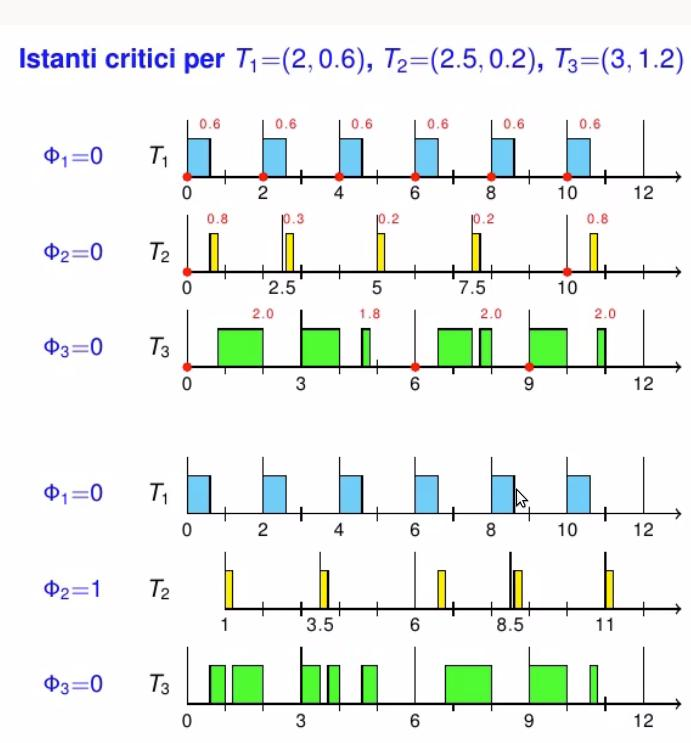
\includegraphics[scale=0.4]{immagini/image-001.jpg}
\end{figure}
Stesso esempio anche se i task non sono in fase: 6 è istante critico, è descritto dal teorema.\\ Quando c'è rilascio in fase, siccome priorità è fissa, la schedulazione prodotta risulta identica a qualsiasi schedulazione non in fase $\Rightarrow$ mi interessa ricondurmi a quando tutti i task sono in fase.
\subsection{Schedulabilità per priorità fissa e tempi di risposta piccoli}
Supponiamo che in un sistema ho task a priorità fissa e tempi di risposta piccoli.\\ Ordino i task per priorità decrescente, suppongo siano in fase all'istante t$_{0}$.\\ Ho i task T$_{1}$......T$_{i}$ e mi chiedo il tempo necessario per eseguire tutti i job dei task T$_{1}$......T$_{i}$, nell'intervallo [t$_{0}$, t$_{0}$+t] (t $\leq$ p$_{i}$:\\
w$_{i}$(t) = e$_{i}$ +  $\sum\limits_{k=0}^{i-1} \lceil\frac{t}{p_{k}}\rceil \cdot e_{k}$.\\ Somma si estende su tutti i task di priorità superiore di T$_{i}$, devo considerarli perché portano via tempo al job di T$_{i}$. Prendo k-esimo task: a t$_{0}$ tutti i task sono in fase, quindi rilascio sicuro un job, quando ne rilascio? Prendo il ceil di $\frac{t}{p_{k}}$,anche job rilasciato nel periodo dopo quello considerato mi ruba tempo; moltiplico tutto per e$_{k}$, il tempo che ci metto per completare i job.\\ Test di schedulabilità: dati job T$_{1}$......T$_{i}$, in fase a t$_{0}$ con priorità decrescenti con T$_{1}$......T$_{i-1}$ effettivamente schedulabili. Il task T$_{i}$ può essere schedulato nell'intervallo di tempo [t$_{0}$, t$_{0}$+D] se $\exists$ t $\leq$ D$_{i}$ tale che w$_{i}$(t) $\leq$ t. IL mio scopo è sempre quello di verificare la schedulabilità del sistema, se ne trovo uno non schedulabile la mia analisi è finita, non ci faccio nulla col sistema di task.\\ Applicazione: ho T$_{1}$......T$_{n}$ con priorità decrescenti. \\Considero un task alla volta: $\forall$ task T$_{i}$  calcolo il valore della funzione di tempo necessario w$_{i}$(t) per tutti i valori t $\leq$D$_{i}$ tali per cui t è un multiplo intero di p$_{k}$ per k $\in$ \{1,2....,i \}.Funzione w$_{i}$(t) sale a gradini, devo considerare valori per cui tale funzione cambia valori.\\ Se per almeno uno dei valori t vale che w$_{i}$(t) $\leq$ t allora T$_{i}$ è effettivamente schedulabile. Altrimenti il test fallisce, ovvero n job di T$_{i}$ potrebbe mancare la scadenza, ovvero la manca sicuro se c'è un rilascio di tutti i job in fase dei task di priorità superiore e tutti quei task hanno un tempo di esecuzione pari al loro worst-case.\\ Possono esserci casi fortuiti, quindi in ipotesi rilassate il test non conferma schedulabilità ma scheduler riesce, però il risultato non è rilevante.\\Tanto vale fermarsi e riprogettare il sistema.\\
esempio: T$_{1}$=(3,1), T$_{2}$=(5,1.5), T$_{3}$=(7, 1.25), T$_{4}$=(9,0,5) e considero le funzioni di tempo necessario:\\
\begin{figure}[!h]
\centering
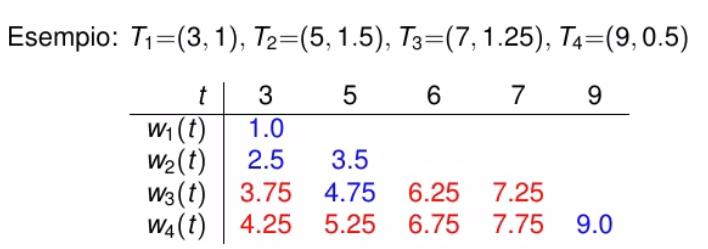
\includegraphics[scale=0.4]{immagini/image-002.jpg}
\end{figure}
Grafico per l'esempio precedente, ho la bisettrice del 1° quadrante, dire che w$_{i}$(t) è $\leq$ t vuol dire che w$_{i}$(t) sta sotto la bisettrice. La funzione è a scalini, non ha senso calcolarla, la applico nel periodo tra 0 e la fine del periodo.In T$_{2}$ la funzione sale sopra la bisettrice, ma non è importante: devo verificare che sia sotto in un certo momento, se fosse sempre sopra non sarebbe schedulabile.\\ Ogni volta che c'è rilascio di un task a priorità superiore $\Rightarrow$ ho gradino nella funzione di tempo necessario.\\
\begin{figure}[!h]
\centering
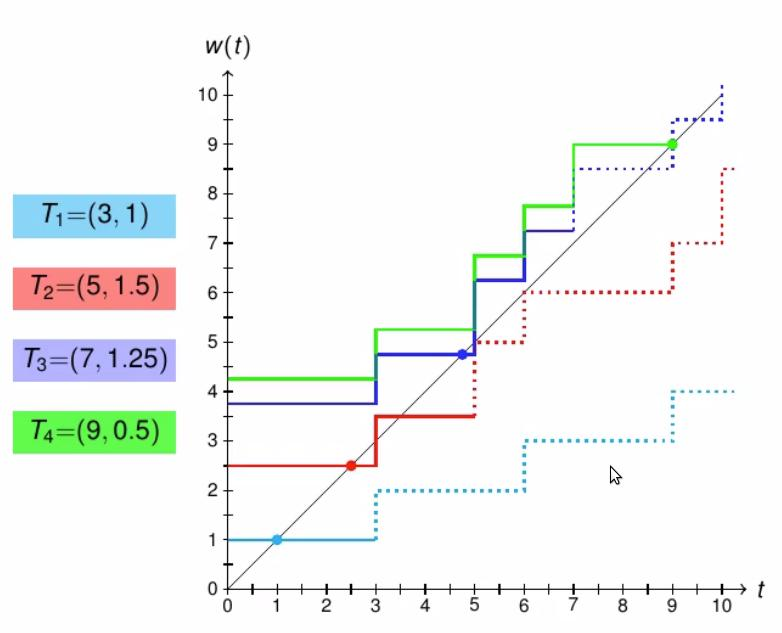
\includegraphics[scale=0.4]{immagini/image-003.jpg}
\end{figure}
\subsection{Massimo tempo di risposta}
Massimo tempo di risposta W$_{i}$ di T$_{i}$ è il più piccolo valore prima della scadenza relativa t.c : t=w$_{i}$(t). Se l'equazione non ha soluzioni $\leq$ a D$_{i}$, allora qualche job di T$_{i}$ mancherà la scadenza relativa.\\ Uso un algoritmo:\\
\begin{itemize}
\item $t^(1)$ = e$_{1}$ in prima approssimazione
\item  Sostituisco nella funzione ed ottengo un nuovo valore $t^(k+1)$ = w$_{i}$($t^(k)$)
\item continuo ad iterare finché: 
\begin{itemize}
\item $t^(k+1)$ = $t^(k)$ e $t^(k)$ $\leq$ D$_{i}$ $\Rightarrow$ W$_{i}$ = $t^(k)$
\item $t^(k)$ $\geq$ D$_{i}$ e allora sono fuori scadenza
\end{itemize}
\end{itemize}
Ma dato che caso peggiore sono task in fase e dato che ho tutti i parametri sono noti, non sarebbe più facile provare a simulare la schedulazione? Sì, ma ci sono dei fattori che non ho considerato e che mi impediscono di simulare, esempio:
\begin{itemize}
\item Non è possibile determinare facilmente il worst case
\item Il worst case cambia da task a task
\item È difficile integrare nella simulazione altri fattori che possono essere considerati estendendo il test di schedulabilità.
\end{itemize}
In ogni caso, sia simulare il test che il test di schedulabilità stesso hanno la stessa complessità.
\subsubsection{Task periodici con tempi di risposta arbitrari}
Considero ora task con tempi di risposta arbitrari, che implica che: 
\begin{itemize}
\item Un job non deve necessariamente prima che il job successivo dello stesso task sia eseguito
\item è possibile che D$_{i}$ $\geq$ di p$_{i}$
\item Ci possono essere nello stesso istante più job di uno stesso task in attesa di essere eseguiti.
\item Un job rilasciato contemporaneamente a tutti i job dei task con priorità maggiore non ha necessariamente il massimo t. di risposta possibile.
\end{itemize}
Assumo sempre che i job di uno stesso task hanno vincoli di precedenza impliciti fra di loro, ovvero sempre eseguiti FIFO.\\ Analizzo task per task: considero T$_{i}$ (i precedenti sono schedulabili). Ho insieme task $\tau_{i}$=T$_{1}$....T$_{i}$ con priorità decrescente. \\Definisco un intervallo totalmente occupato di un livello $\pi_{i}$ un intervallo (t$_{0}$, t$_{1}$] tale che:
\begin{itemize}
\item all'istante t$_{0}$ tutti i job di $\tau_{i}$ rilasciatiti prima di t$_{0}$ sono stati completati
\item All'istante t$_{0}$ un job di $\tau_{i}$ viene rilasciato.
\item L'istante t$_{1}$ è il primo istante in cui tutti i job di $\tau_{i}$ rilasciati a partire da t$_{0}$ sono stati completati
\end{itemize}
È possibile che in un intervallo totalmente occupato il processore sia idle o esegua task non di $\tau_{i}$? No: se fosse idle, l'intervallo terminerebbe prima, non può neanche eseguire task di priorità inferiore, quindi non può eseguire task al di fuori di $\tau_{i}$\\
esempio: T$_{1}$, T$_{2}$, T$_{3}$.\\ Intervalli di T$_{3}$ non sono lunghi uguale, questo perché i rilasci di T$_{3}$ non sono in concomitanza con T$_{1}$ e T$_{2}$, posso dire che l'intervallo a lunghezza massimo quando i rilasci di tutti i task sono in fase.\\ Test di schedulabilità generale per tempi di risposta arbitrari è ancora basato sul caso peggiore, la differenza rispetto al test per tempi piccoli è che il primo job rilasciato contemporaneamente agli altri potrebbe non avereil massimo tempo di risposta.\\ Idea : $\forall$ T$_{i}$ analizzo tutti i suoi job eseguiti nel primo intervallo totalmente occupato di livello $\pi_{i}$. \\ Come determino l'intervallo totalmente occupato: 
\begin{itemize}
\item Inizio determinato dal rilascio dei primi job (in fase) dei task $\tau_{i}$=\{T$_{1}$, ...., T$_{i}$\}
\item Lunghezza massima calcolata risolvendo iterativamente t = $\sum\limits_{k=1}^{i}\lceil\frac{t}{p_{k}}\rceil \cdot e_{k}$. Molto simile alla funzione di tempo necessario, dico che aumento t fino a che non trovo il valore dato dalla sommatoria, ovvero il primo t per cui il lavoro necessario per compiere tutti i task permette di eseguire tutti i task rilasciati nell'intervallo [t$_{0}$, t$_{0}$+t] 
\end{itemize}
Quindi si procede nel seguente modo:
\begin{itemize}
\item Considero i task \{T$_{1}$, ...., T$_{i}$\} con priorità $\pi_{1}$ $<$ $\pi_{2}$....$<$ $\pi_{i}$, considero un task T$_{i}$ alla volta cominciando da quello con la massima priorità, ovvero T$_{1}$
\item Il caso peggiore per la schedulabilità di T$_{i}$: assumere che i task $\tau$ $_{i}$ = \{T$_{1}$, ...., T$_{i}$\} sono in fase.
\item Se il primo job di tutti i task in $Tau_{i}$ termina entro il primo periodo del task $\Rightarrow$ decidere se T$_{i}$ è  schedulabile si effettua controllando se J$_{i,1}$ termina entro la scadenza tramite la funzione di tempo richiesto w$_{i,1}$ := w$_{i}$(t)
\item Altrimenti almeno un primo job di $Tau_{i}$ termina dopo il periodo del task, calcola la lunghezza $t^L$ dell'intervallo totalmente occupato di livello $\pi_{i}$ che inizia da t = 0.
\item Calcolo i tempi di risposta massimi di tutti i job di T$_{i}$ dentro l'intervallo totalmente occupato che sono $\lceil$ $\frac{t^L}{p_{i}}$ $\rceil$; il primo l'ho già calcolato.
\item Decido se questi job sono schedulabili dentro l'intervallo totalmente occupato. Uso un lemma:\\
Il tempo di risposta massimo W$_{i,j}$ del j-esimo job di T$_{i}$, in un intervallo totalmente occupato di livello $\pi_{i}$ in fase è uguale al minimo t che soddisfa l'equazione t = w$_{i,j}$(t+(j-1)$\cdot$ p$_{i}$) - (j-1)$\cdot$ p$_{i}$, con w$_{i,j}$(t) = j$\cdot$e$_{i}$ + $\sum\limits_{k=1}^{i-1}\lceil\frac{t}{p_{k}}\rceil \cdot e_{k}$.\\ Aggiungo un j che moltiplica e$_{i}$, devo verificare l'equazione nei punti multipli.\\ 
\end{itemize}
esercizio:
T$_{1}$ = ($\phi_{1}$,2,1,1), T$_{2}$ = ($\phi_{2}$,3,1.25,4), T$_{3}$ = ($\phi_{3}$,5,0.25,7)\\ Parto verificando T$_{1}$: \\w$_{1}$(t) = w$_{1,1}$(t) = e$_{1}$ = 1 = D$_{1}$. Quindi è sicuramente schedulabile . \\T$_{2}$:\\
w$_{2,1}$(2) = e$_{1}$ + e$_{2}$ = 2.25 $>$ 2, quindi non va bene. Vado avanti: \\
w$_{2,1}$(3) = 2$\cdot$e$_{1}$ + e$_{2}$ = 3.25 $>$ 3. Non va ancora bene, proseguo: \\
w$_{2,1}$(4) = 2$\cdot$e$_{1}$ + e$_{2}$ = 3.25 $\leq$ 4 $\leq$ $D_{2}$ quindi T$_{2}$ è schedulabile, ma ha completato oltre il periodo $\Rightarrow$ non posso più considerare tempi piccoli, devo considerare gli intervalli totalmente occupati, uso l'equazione iterativa:\\
$t^(1)$ = e$_{1}$ + e$_{2}$ = 2.25, sostituisco nella sommatoria,ed ottengo $t^(2)$ = 2$\cdot$e$_{1}$ + e$_{2}$ = 3.25, $t^(3)$ = 2$\cdot$e$_{1}$ + 2$\cdot$e$_{2}$ = 4.5, $t^(4)$ = 3$\cdot$e$_{1}$ + 2$\cdot$e$_{2}$ = 5.5, $t^(5)$ = 3$\cdot$e$_{1}$ + 3$\cdot$e$_{2}$ = 5.5 $\Rightarrow$ $t^(4)$ = $t^L$, ovvero intervallo totalmente occupato di livello 2 è 5.5.\\ Ora calcolo quanti job di T$_{2}$ ci sono in (0, 5.5] = $\lceil$ $\frac{t^L}{p_{2}}$ $\rceil$ = 2.\\ Veridico il secondo job di T$_{2}$:\\
w$_{2,2}$(3) = 2$\cdot$e$_{1}$ + 2$\cdot$e$_{2}$ = 4.5 $>$ 3, no\\
w$_{2,2}$(4) = 2$\cdot$e$_{1}$ + 2$\cdot$e$_{2}$ = 4.5 $>$ 4, ancora no.\\
w$_{2,2}$(3) = 3$\cdot$e$_{1}$ + 2$\cdot$e$_{2}$ = 5.5 $\leq$6 $\leq$ $p_{2}$+$D_{2}$=7, quindi accetto il task.\\ Ora devo capire  se posso accettare T$_{3}$, e considerare l'intervallo totalmente occupato di lvl 3:\\ 
$t^(1)$ = e$_{1}$ + e$_{2}$ +e$_{3}$ = 2.5\\
$t^(2)$ = 2$\cdot$e$_{1}$ + e$_{2}$ +e$_{3}$ = 3.5\\
$t^(3)$ = 2$\cdot$e$_{1}$ + 2$\cdot$e$_{2}$ +e$_{3}$ = 4.75\\
$t^(4)$ = 3$\cdot$e$_{1}$ + 2$\cdot$e$_{2}$ +e$_{3}$ = 5.75\\
$t^(5)$ = 3$\cdot$e$_{1}$ + 2$\cdot$e$_{2}$ + 2$\cdot$e$_{3}$ = 6\\
$t^(6)$ = 3$\cdot$e$_{1}$ + 2$\cdot$e$_{2}$ + 2$\cdot$e$_{3}$ = 6 = $t^L$\\
\# job di T$_{3}$ nell'intervallo (0,6]: $\lceil$ $\frac{t^L}{p_{3}}$ $\rceil$ = 2. Considero i  singoli job:\\
w$_{3,1}$(2) = e$_{1}$ + e$_{2}$ + e$_{3}$ = 2.5 $>$ 2, no.\\
w$_{3,1}$(3) = 2$\cdot$e$_{1}$ + e$_{2}$ + e$_{3}$ = 3.5 $>$ 3, no.\\
w$_{3,1}$(4) = 2$\cdot$e$_{1}$ + 2$\cdot$e$_{2}$ + e$_{3}$ = 4.75 $>$ 4, no.\\
w$_{3,1}$(5) = 3$\cdot$e$_{1}$ + 2$\cdot$e$_{2}$ + e$_{3}$ = 5.75 $>$ 5, no.\\
w$_{3,1}$(6) = 3$\cdot$e$_{1}$ + 2$\cdot$e$_{2}$ + e$_{3}$ = 5.75 $\leq$ 6 $\leq$ D$_{3}$ = 7. Posso accettare il job\\\\
w$_{3,2}$(5) = 3$\cdot$e$_{1}$ + 2$\cdot$e$_{2}$ + 2$\cdot$e$_{3}$ = 6 $>$ 5, no.\\
w$_{3,2}$(6) = 3$\cdot$e$_{1}$ + 2$\cdot$e$_{2}$ + 2$\cdot$e$_{3}$ = 6 $\leq$ 6 $\leq$ p$_{3}$ + D$_{3}$ = 12 Accetto il job, e quindi il task.\\ Tutti i task sono schedulabili a prescindere dai loro task.\\ 
\subsection{Condizioni di schedulabilità}
Il test di schedulabilità generale determina se insieme di task è schedulabile o no, considerando worst case che è task in fase.\\ Ho dei limiti:
\begin{itemize}
\item Devo conoscere tutti i periodi, le scadenze ed i tempi d'esecuzione. Per validazione è necessario, ma no per implementazione di scheduler a priorità fissa. Se voglio aggiungere un task dovrei conoscere parametri che in fase di progettazione del sw non servono.
\item Il risultato ottenuto non è valido se il task varia periodo, scadenza o tempo di esecuzione.
\item È computazionalmente costoso, poco adatto per scheduling on-line.
\end{itemize}
Cerco di trovare delle condizioni di schedulabilità, confronto il test con la condizione, che è molto più semplice da calcolare e che può essere applicata anche se alcuni parametri non sono noti (esempio: condizione di EDF).\\ Mi chiedo se $\exists$ condizione di schedulabilità per algoritmi a priorità fissa:\\ Condizione di Liu-Layland: sistema $\tau$ di n task indipendenti ed interrompibili con scadenze relative uguali ai rispettivi periodi può essere effettivamente schedulato su un processore in accordo con RM se il suo fattore di utilizzazione U$_{\tau}$ è $\leq$ a U$_{RM}$(n) = n$\cdot$($2^{\frac{1}{n}}$-1)\\ Questo è il fattore di utilizzazione di RM, se considero: $\lim_{n \to \inf}$ U$_{RM}$(n) = ln2, ovvero RM in generale garantisce di rispettare le scadenze pur di non caricare il processore per più del 69.3.\\ Ho un criterio per adottare RM negli scheduler real-time.\\ esempio:\\ T$_{1}$ = (1,0.25), T$_{2}$ = (1.25,0.1), T$_{3}$ = (1.5,0.3), T$_{4}$ = (1.75,0.07), T$_{5}$ = (2,0.1). U$_{\tau}$ = 0.62 $\leq$ 0.743 = U$_{RM}$(5) $\Rightarrow$ è schedulabile con RM.\\ IL sistema T$_{1}$ = (3,1), T$_{2}$ = (5,1.5), T$_{3}$ = (7,1.25), T$_{4}$ = (9,0.5) ha fattore di utilizzazione U$_{\tau}$ = 0.867 $>$ 0.757 = U$_{RM}$(4),  forse non schedulabile.\\ È condizione sufficiente, difatti l'esempio 2 era quello precedente che è schedulabile se applico la funzione di tempo necessario.\\ L'alternativa a questo risultato è il test iperbolico: Un sistema $\tau$ di n task indipendenti ed interrompibili con scadenze relative uguali ai rispettivi periodi può essere effettivamente schedulato su un processore RM se $\prod\limits_{k=1}^{n}(1 + \frac{e_{k}}{p_{k}})$ $\leq$ 2.\\ SI applica anche questo conoscendo solo fattore di utilizzazione dei task. \\ Correlazione con condizione di Liu-Layland: se gli n task hanno tutti lo stesso rapporto $\frac{e_{k}}{p_{k}}$ vuol dire che ciascun di questi usa una porzione uguale del processore. \\ Si può dimostrare che se questo è vero allora, assumendo u$_{k}$ = $\frac{U_{\tau}}{n}$:\\
$\prod\limits_{k=1}^{n}(1 + \frac{e_{k}}{p_{k}})$ $\leq$ 2 $\Leftrightarrow$ U$_{\tau}$ $leq$ n$\cdot$($2^{\frac{1}{n}}$-1). \\Se questo non è vero, esistono casi in cui il test iperbolico è soddisfatto, ma la condizione di Liu-Layland no; non esiste invece mai il viceversa.\\
\subsection{Test per sottoinsiemi di task armonici}
So che ,in generale RM è schedulabile se è soddisfatta condizione di Liu-Layland, ma so anche che su task armonici è ottimale. Suddivido insiemi di task in sottoinsiemi di task armonici fra loro.\\ Condizione di Kuo-Mok: se sistema $\tau$ di task periodici, indipendenti ed interrompibili con p$_{i}$ = D$_{i}$ può essere partizionato in n$_{h}$ sottoinsiemi disgiunti Z$_{1}$,....,Z${n_{h}}$, ciascuno dei quali contiene task semplicemente periodici, allora il sistema è schedulabile con RM se:\\
$\sum\limits_{k=1}^{n_{h}}U_{Z_{k}}(n_{h})$ oppure se $\prod\limits_{k=1}^{n_{h}}(1+U_{Z_{k}})$ $\leq$ 2.\\ Se un sistema ha poche applicazioni molto complesse, è possibile migliorare la schedulabilità rendendo i task di ciascuna applicazione semplicemente periodici.\\ Esempio: 9 task con periodi 4,7 ,7 , 14, 16, 28, 32, 56, 64, fattore di utilizzazione di Liu-Layland è U$_{RM}$ = 0.720\\ Considero i multipli di 2 e 7 e partizionando in due sottoinsiemi ottengo U$_{Z_{1}}$ + U$_{Z_{2}}$ $\leq$ U$_{RM}$(2) = 0.828.\\\\ Il fattore di RM è in generale U$_{RM}$(n), ma posso farlo diventare pari ad 1 per task semplicemente periodici.\\ Miglioro U$_{RM}$(n) considerando quanto i periodi dei task sono vicini ad essere armonici:\\
X$_{i}$ = log$_{2}$p$_{i}$ - $\lfloor$ log$_{2}$p$_{i}$ $\rfloor$ e $\zeta$ = max$_{1 \leq i \leq n}$X$_{i}$ - min$_{1 \leq i \leq n}$X$_{i}$\\ Considero il valore frazionario del log$_{2}$ e prendo tutti i task, di cui faccio differenza tra max e min di questi scarti decimali.\\ Teorema: nelle ipotesi della condizione di Liu-Layland, il fattore di utilizzazione di RM dipende dal numero di task n e da $\zeta$ è: 
U$_{RM}$(n, $\zeta$) =
\begin{itemize}
\item (n-1)$\cdot$($2^\frac{\zeta}{(n-1)}$-1) + $2^{(1-\zeta)}$-1  se $\zeta$ $<$ 1 - $\frac{1}{n}$
\item U$_{RM}$(n)
\end{itemize}
Quando si verifica il caso $\zeta$ = 0? Quando p$_{i}$ = K$\cdot$ $2^{x_{i}}$; non è vero il contrario\\
Variante: schedulabilità per scadenze arbitrarie. Se per qualche task la scadenza è più grande del periodo il limite è valido? Sì, però la formula è "pessimista": forse è possibile trovare valori di soglia superiori a U$_{RM}$.\\ Se invece per qualche task il periodo è più grande della scadenza non posso applicare Liu-Layland.\\ Teorema:	\\
Un sistema $\tau$ di n task indipendenti, interrompibili e con scadenze D$_{i}$ = $\delta$p$_{i}$ è schedulabile con RM se U$_{\tau}$ è $\leq$ a:
U$_{RM}$(n, $\delta$) =
\begin{itemize}
%\begin{cases}
\item $\delta$(n-1)$\cdot$($\frac{\delta+1}{\delta}^{\frac{1}{(n-1)}}$ - 1)  per $\delta$ = 2,3,.....
\item n($2\delta^{\frac{1}{n}}$-1) + 1 - $\delta$ per 0.5 $\leq$ $\delta$ $\leq$ 1
\item $\delta$ per 0 $\leq$ $\delta$ $\leq$ 0.5
%\end{cases}
\end{itemize}
\chapter{Schedulazione di job bloccanti e job aperiodici}
\section{Schedulazione di job bloccanti e job aperiodici}
Avevo un modello semplice, devo rilassare qualcuna delle ipotesi dovute al fatto che i job siano sempre sempre interrompibili, o che costo di context switching sia 0. Nella pratica molti fattori rallentano l'esecuzione di un job, che possono portare a mancata scadenza. Devo tenerne conto, divido in due genti classi:
\begin{itemize}
\item Tempi di blocco: job non può essere eseguito nonostante il rilascio, per via di fattori esterni. Ad esempio: sul processore c'è un job non interrompibile, job rilasciato è quindi bloccato per un certo tempo. Modellati definendo b$_{i}$ = tempo massimo di blocco, che tiene conto di tutti i tempi che fanno si che il job non può eseguire, va sottratto al tempo a disposizione del job.
\item rallentamenti sistematici: ho calcolato il worst case di un job, ma a questo devo considerare il tempo che ci mette il job ad essere posto in esecuzione e ad essere tolto una volta completato, o anche il tempo che ci mette lo scheduler a decidere. Se questo tempo ha impatto pratico può avere senso modellarlo. Sommo al worst case del job.
\end{itemize}
\subsection{Auto-sospensione}
Un job rilasciato non può essere eseguito perché in attesa di eventi esterni, la cosa migliore da fare in questi casi è mettere in esecuzione un altro job. Si dice che il job si è auto-sospeso:
\begin{itemize}
\item job è un processo ed esegue operazione di accesso alla memoria di massa, ha senso sostituire il processo mentre questo attende i dati.
\item attendo dati da rete/altri job
\item attendo scadenza di un timer
\end{itemize}
Nei SO questo tipo di operazioni sono chiamate operazioni bloccanti, nell'ambito real-time ci possono essere operazioni di auto-sospensione che però non è bloccante: in questo ambito ha senso attivo, ovvero un job ne blocca un altro. Anche in questo caso ci sono conseguenze su un altro job.\\ Supponiamo che ogni job di un task T$_{i}$ si auto-sospende per un certo tempo x, in questo caso non appena rilasciato. Come schedulo: considero l'istante di rilascio come p$_{i}$-x, e la scadenza relativa come D$_{i}$-x.\\ Approccio semplificato, non funziona nel caso in cui i job si auto-sospendono solo all'inizio o per un tempo determinato, devo definire il tempo massimo di auto-sospensione b$_{i}$(ss).\\ esempio: T$_{1}$ = (4, 2.5) T$_{2}$ = (3.7, 2, 7) schedulato con RM. Se primo job di T$_{1}$ si auto-sospende subito dopo il rilascio, le cose possono andare male: il primo job del task T$_{2}$ manca la scadenza, job di T$_{1}$ si risveglia in modo che per completare occupa tutto il suo periodo, quindi quando job di T$_{2}$ comincia esecuzione di porta avanti ma non riesce a finire.\\
\begin{figure}[!h]
\centering
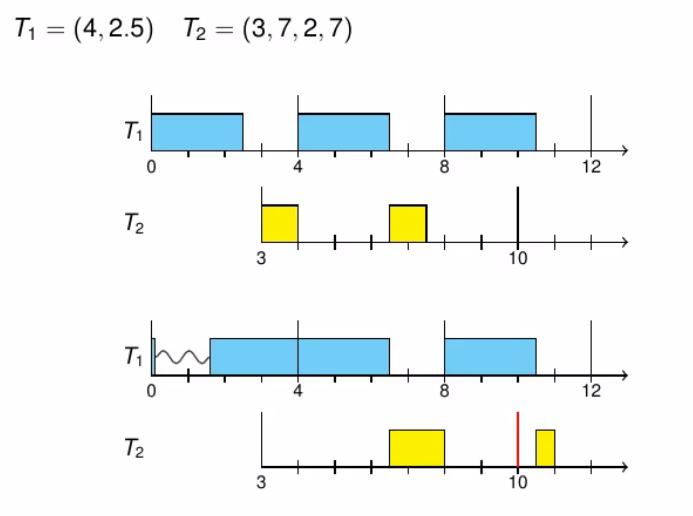
\includegraphics[scale=0.4]{immagini/image-004.jpg}
\end{figure}
Ho impatto sui job di priorità inferiore: anche se job si auto-sospende on no lo fa, se c'è job di priorità superiore non è danneggiato, ma quelli di priorità inferiore si.
\subsubsection{Rallentamento dovuto all'auto-sospensione}
1° caso: il tempo di auto-sospensione di un job è maggiore della durata del job: job di T$_{i}$ con priorità inferiore è rallentato al massimo per un tempo pari alla durata del job di T$_{k}$ È il worst case: job T$_{i}$ non riesce ad arrivare mente job di T$_{k}$ è in auto-sospensione\\
\begin{figure}[!h]
\centering
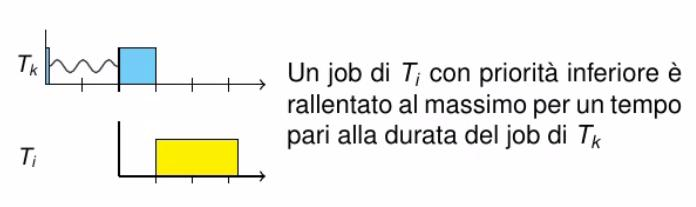
\includegraphics[scale=0.4]{immagini/image-005.jpg}
\end{figure}
2° caso: il tempo di auto-sospensione di un job è minore della durata del job. Un job di T$_{i}$ con priorità minore è rallentato al massimo per un tempo pari alla durata dell'auto sospensione.\\
\begin{figure}[!h]
\centering
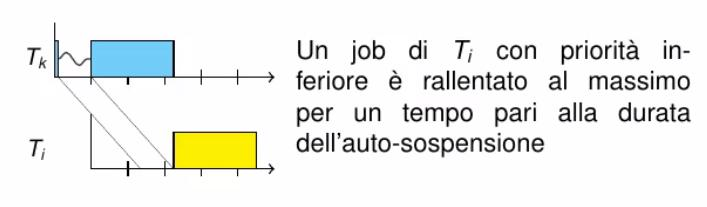
\includegraphics[scale=0.4]{immagini/image-006.jpg}
\end{figure}
\subsubsection{Tempo massimo di sospensione di blocco per auto-sospensione}
Dato task T$_{k}$ chiamo x$_{k}$ il tempo massimo di sospensione di ciascun job di T$_{k}$, questo è un parametro del sistema.\\ Prendo task T$_{i}$ con priorità minore, il rallentamento inflitto ad un job T$_{i}$ da un job di T$_{k}$ è minore o uguale ad x$_{k}$ e minore o uguale ad e$_{k}$:
b$_{i}$(ss) = x$_{i}$ + $\sum\limits_{k = 1}^{i-1}min(e_{k}, x_{k})$.\\ Manca qualcosa, sto assumendo che un job si auto-sospenda una volta sola, ma non c'è nessun motivo reale per cui questo sia vero: job può auto-sospendersi più volte, devo contare il numero di volte. Devo definire anche il massimo numero di volte k$_{i}$ in cui un job di T$_{i}$ si sospende.\\ Difatti:
\begin{itemize}
\item si può verificare un blocco da parte di un processo non interrompibile
\item si ha un rallentamento dovuto allo scheduler ed al costo del context switching
\end{itemize}
\subsection{Non interrompibilità dei job}
Assunzione irrealistica che i job non siano interrompibili, esistono sempre istanti in cui il job non è interrompibile:
\begin{itemize}
\item se sta operando su area di memoria critica
\item se sta interagendo con dispositivo hardware
\item job esegue syscall, e ci sono chiamate di sistema che non possono essere interrotte.Job diventa non interrompibile fino alla conclusione del SO.
\item costo del context switch è troppo elevato
\end{itemize}
Un job J$_{i}$ è bloccato per non interrompibilità quando è  pronto per essere eseguito, ma non può perché è in esecuzione un job non interrompibile.\\ Quando si verifica questo fenomeno, si parla di inversione di priorità quando la priorità del job in esecuzione è minore di quella del job pronto per l'esecuzione. esempio: T$_{1}$ = ($\epsilon$, 4, 1, 4), T$_{2}$ = ($\epsilon$, 5, 1.5, 5), T$_{3}$ = (9, 2). Qualunque sia l'algoritmo, all'istante 0 viene messo in esecuzione job di T$_{3}$, inoltre U = 0.77 ed è schedulabile per EDF e RM, ma solo se job sono non interrompibili. Suppongo che T$_{3}$ non sia interrompibile, conclude nell'istante 2, quindi tra [$\epsilon$,2] blocca due job con priorità maggiore. Nell'intervallo tra [2, 5+$\epsilon$] eseguo 3 job, 2 di T$_{1}$ ed uno di T$_{2}$, ma non c'è abbastanza tempo e quindi T$_{2}$ manca la scadenza.\\ 
\begin{figure}[!h]
\centering
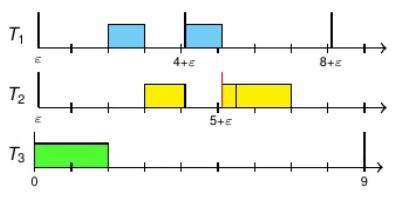
\includegraphics[scale=0.4]{immagini/image-007.jpg}
\end{figure}
\\Come faccio a modellare che il job è non interrompibile, devo capire la durata massima di non interrombilità di un job: sia $\\Theta_{k}$ il tempo di esecuzione massimo della più lunga sezione non interrompibile dei job di T$_{k}$. Sia b$_{i}$(np) il tempo massimo di blocco per non interrompibilità, che è tempo subito da un job a causa dei job di priorità inferiore, quando vale? b$_{i}$(np) = max\{$\Theta_{k}$: per ogni task T$_{k}$ di priorità minore a T$_{i}$ \}: suppongo che c'è job di alta priorità rilasciato, ho sul processore job di priorità inferiore T$_{k}$ appena entrato nella sezione critica non interrompibile più lunga, subisco rallentamento di $\Theta_{k}$, ma appena finisce la sezione lo scheduler da la priorità a me, non importa quanto solo lunghe le sezioni degli altri job: caso peggiore è che vengo rilasciato quando il job che ha il $\Theta_{k}$ più lungo entra in esecuzione.\\ Il tempo massimo di blocco totale dipende da entrambe i due tempi di blocco:
b$_{i}$ = b$_{i}$(ss) + (K$_{i}$+1) $\cdot$ b$_{i}$(np). Considero numero massimo di volte per cui il job J$_{i}$ si sospende, il +1 è il fatto che la prima volta deve essere rilasciato sia che si auto-sospende che non.
\subsection{Cambi di contesto}
Come modellare rallentamenti dovuti al context switch: CS= context switch time, per ora ci metto anche tempo necessario per lo scheduler per prendere decisione.\\ Allungo il worst case del job: calcolato quando non c'è nulla che interferisce col job. worst case è e'$_{i}$ = e$_{i}$ + 2 $\cdot$ (K$_{i}$ + 1) $\cdot$ CS. job deve subire almeno due cambi di contesto: quando viene messo in esecuzione e quando viene tolto dall'esecuzione.Ma ogni volta che il job si auto-sospende  c'è un altro cambio di contesto: per essere tolto e poi per essere rimesso; K$_{i}$ = n° volte che il job si auto-sospende.\\ Alle volte non è utile modellare il context switch, però in altri casi è essenziale farlo: LST si basa sullo slack rimanente, quindi ci sono molti cambi di contesto e l'overhead è significativo ed è doveroso modellarli. Con LST è anche spesso difficile capire qual'è numero massimo di context switch di job, ma ci sono algoritmi come EDF altrettanto buoni, in un sistema real-time parametro cruciale: i job devono rispettare le scadenze; utiele vederlo in teoria ma non in pratica.
\subsection{Test di schedulabilità per job bloccanti}
Come faccio ad usare i parametri definiti nel processo di validazione: o uso test di schedulabilità o uso condizioni di schedulabilità.\\ Idea è che tempo disponibile per completare per ciascun job va diminuito del tempo massimo per cui quel job può rimanere bloccato, definisco tempo di blocco come tempo max aggiuntivo. La funzione di tempo massimo richiesto diventa:\\
w$_{i}$(t) = e$_{i}$ + b$_{i}$ + $\sum\limits_{k = 1}^{i-1}\lceil \frac{t}{p_{k}} \cdot e_{k} \rceil$ per 0 $<$ t $\leq$ min(D$_{i}$, p$_{i}$). Ho meno tempo a disposizione per completare il job, sommo b$_{i}$.\\ Stesso si applica al test di schedulabilità generale:\\
w$_{i,j}$(t) = j $\cdot$ e$_{i}$ + b$_{i}$ + $\sum\limits_{k = 1}^{i-1}\lceil \frac{t}{p_{k}} \cdot e_{k}$  per (j-1)$\cdot$ p$_{i}$ $<$ t $\leq$ w$_{i,j}$(t). non devo moltiplicare b$_{i}$ per j: il 3° job di T$_{i}$ è sempre 3$ \cdot$ e$_{i}$, ma sto cercando di capire quanto tempo rimane al 3° job, perché questo viene bloccato solo per b$_{i}$. Il blocco è qualcosa che considero soltanto quando devo studiare la schedualbilità del singolo job ed è relativa solo al singolo job. Non ha senso considerarla per tutti i task insieme, si fa sempre studio task per task.
\subsection{Condizioni di schedualbilità per task bloccanti +a priorità fissa}
Sia dato sistema di n task T ed un algoritmo a priorità fissa X, con fattore di utilizzazione U$_{X}$(n). Sappiamo che il sistema è effettivamente schedulabile se U$_{T}$ $\leq$ U$_{X}$(n), a condizione che i task non blocchino mai. Come adatto la condizione per task a priorità fissa ma che bocchino? Non posso più usare solo le condizioni di schedualbilità, perché ciascun job può bloccare con misura differente, quindi devo farlo per un task alla volta. Nel caso peggiore, ogni job di T$_{i}$ impiega un tempo e$_{i}$ + b$_{i}$ per completare l'esecuzione. Posso modellare questo tempo come tempo di esecuzione in più che il job deve subire: dato un task T$_{i}$, calcolo utilizzazione totale fino alla priorità i, dato task calcolo utilizzazione totale fino alal priorità i:\\ $\sum\limits_{k = 1}^{i}\frac{e_{k}}{p_{k}} + \frac{b_{i}}{p_{i}}$ $\leq$ U$_{X}$(i). Task di priorità inferiore non possono incidere sulla priorità del task, o meglio lo faranno solo se sono non bloccanti ma lo sto già considerando. Guardo solo ai task con priorità maggiore, considero come n° task solo fino ad i, considero solo U$_{X}$(i), man mano arriverò ad U$_{X}$(n).
Applico anche ad EDF, considero task per task, parlo in generale di densità ed uso approccio simile al precedente: task per task questo è schedualbile se:\\ $\sum\limits_{k = 1}^{n}\frac{e_{k}}{min(D_{k}, p_{k})}$ + $ \frac{b_{i}}{min(D_{i}, p_{i})}$ = $\Delta_{\tau}$ + $\frac{b_{i}}{min(D_{i}, p_{i})}$ $\leq$ 1.\\ Non sto parlando di task a priorità fissa, ogni job del sistema può avere priorità che precede il job in questione: di fatto, non posso applicare sommatoria solo a task a priorità superiore ma devo applicare a tutti i task del sistema, quindi arrivare alla densità del sistema. Alla densità contribuisce anche il task in questione che è $ \frac{e_{i}}{min(D_{i}, p_{i})}$, a cui aggiungo anche $ \frac{b_{i}}{min(D_{i}, p_{i})}$ poiché è come se il tempo di esecuzione del job del task è aumentato di b$_{i}$.\\ Problema è definire i tempi massimi di blocco se i task non hanno priorità fissata, la priorità è del job. \\ Teorema (Baker, 1991): in una schedualzione EDF un job con scadenza relativa D può bloccare un altro job con scadenza relativa D' solo se D $>$ D'.\\ Dim: se il job con scadenza relativa D blocca quello con D', vuol dire che la sua priorità è inferiore: bloccare ha il senso che un job a priorità inferiore sta togliendo tempo ad uno a priorità superiore, quindi d $>$ d' (scadenze assolute), per poter bloccare il processore deve averlo messo in esecuzione prima e quindi r $<$ r' $\Rightarrow$ D = d-r $>$ d'-r' = D'.
Ho una soluzione: posso ordinare i task per scadenze relative crescenti, ed applico la formula di b$_{i}$ per i task con priorità fissa.\\ Caso dell'auto-sospensione è difficile, quindi come realizzare il teorema di Baker? Thm non è più valido: se per esempio job J' ha priorità più alta di un job J. Se J' comincia ad eseguire e si auto-sospende: prima di tornare in esecuzione comincia job di priorità più bassa. L'ipotesi che r sia $<$ r' non è più vera, può essere dopo r' semplicemente perché il job si è autosospeso: dovrei applicare al tempo r'+tempo dopo la sospensione.\\ Posso applicare il ragionamento a r'+x'+e': di quanto tempo r può precedere r', sicuramente di x'+e'.Può non precedere r', ma r'+x'+e' è la massima distanza che posso avere fra r ed r'. Formulo teorema di Baker con auto-sospensione: in una schedulazione EDF, un job con scadenza relativa D può bloccare un altro job con scadenza relativa D' e tempo massimo di esecuzione x' solo se D $>$ D'-x'-e'.\\ Dato che entrambi i job possono auto-sospendersi, è possibile che i due task possano bloccarsi a vicenda non ho più ordinamento totale.
\subsection{Schedulazione basata su tick}
Fin'ora ho visto scheduler event-driven: viene eseguito quando si verifica un evento rilevante. In pratica, è più semplice realizzare uno scheduler time-driven, ovvero che si attiva ad interruzioni periodiche: svantaggio è che tutti i tempi nel sistema avranno granularità pari alla dimensione del mio tick.\\ Il riconoscimento di un evento come il rilascio di un job può essere differito fino al tick successivo, è come se ci fosse inversione di priorità. Definisco job pendenti, ovvero che sono stati rilasciati ma che lo scheduler non ha ancora preso in considerazione perché non è scattato il tick, e quelli eseguibili, ovvero quelli piazzati dallo scheduler, ho due code per le rispettivi due classi. Scheduler sposta job da coda dei job pendenti a coda dei job eseguibili.Quando jop termina, so già qual'è il prossimo da eseguire: sarà quello successivo nella coda dei job eseguibili. Se arriva job, questo viene messo nella coda dei job pendenti.
\subsubsection{Test schedulabilità per priorità fissa con tick}
Come posso applicare il test di schedulabilità ad uno scheduler a priorità fissa basato su tick?\\ Considero scheduler che si attiva con periodicità p$_{0}$, esegue in tempo e$_{0}$ il controllo della coda di job pendenti e con CS$_{0}$ trasforma un job da pendente a eseguibile.\\  Per controllare la schedulabilità di T$_{i}$
\begin{itemize}
\item Devo aggiungere task per controllare schedulabilità di un task T$_{0}$ = (p$_{0}$, e$_{0}$) a priorità massima.
\item Devo modellare il fatto che qundo arriva job, questo va prima o poi trasformato da pendente ad eseguibile. 
\begin{itemize}
\item per tutti i task a priorità inferiore rispetto ai job di T$_{i}$, per cui devo tenere conto del fatto che lo scheduler interverrà e trasformerà il job pendente in un job nella coda eseguibile. Oltre ai job di priorità inferiore, che vanno da i+1 a n, aggiungo un numero corrispondete di task T$_{0,k}$ = (p$_{k}$, CS$_{0}$) per ogni k = i+1,..,n, con priorità maggiore di T$_{1}$, ma che hanno periodicità CS$_{0}$, ovvero il tempo che ci mette il processore a trasformare i job in eseguibile da pendenti.
\item job a priorità superiore, aggiungo a tutti i task di priorità superiore o uguale ad (K$_{k}$ + 1) $\cdot$ CS$_{0}$, considero K$_{k}$ perché ogni volta che mi risveglio devo essere spostato da pendente ad eseguibile. Aggiungo questi valori ad e$_{k}$ per ogni k = 1,2...,i.
\end{itemize}
Perché non considero le auto-sospensione per i task a priorità inferiore? Perché task inferiore non viene mai eseguito al posto mio, pago solo il primo rilascio, perché fin quando io sono eseguibile, quelli con meno priorità di me non hanno possibilità di essere eseguiti prima di me.
\item Devo anche considerare il tempo di blocco per non-interrompibilità, anche se tutti i miei job sono sempre non interrompibili. b$_{i}$(np) = ($\lceil max_{i+1 \leq k \leq n}\frac{\Theta_{k}}{p_{0}}\rceil$ + 1) $\cdot$ p$_{0}$. max $\Theta_{k}$ moltiplicato il p$_{0}$ diventa il max di tutti i $\Theta_{k}$ di priorità inferiore, in più c'è un p$_{0}$. esempio:\\
\begin{figure}[!h]
\centering
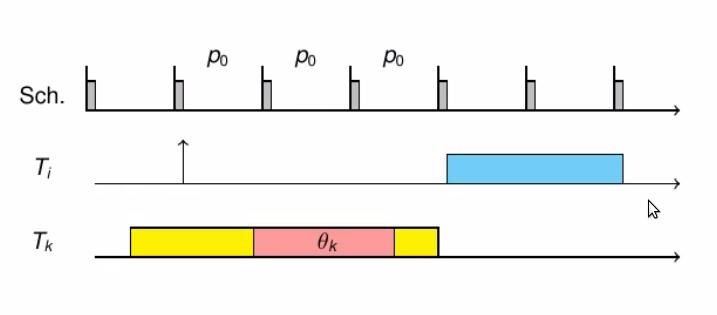
\includegraphics[scale=0.4]{immagini/image-008.jpg}
\end{figure}
ho lo shceduler che viene invocato con periodo p$_{0}$. Ad un certo istante viene rilasciato il job del task T$_{i}$, mi metto nel worst case, ovvero il job T$_{i}$ arriva un infinitesimo dopo che lo scheduler ha finito di controllare la coda dei job pendenti, quindi fino al prossimo p$_{0}$ non potrò eseguire il job. In questo periodo, prima che possa intervenire lo shceduler, si continua ad eseguire un job di priorità inferiore di T$_{k}$ e questo job entra nella regione interrompibile all'interno del periodo p$_{0}$ in cui è arrivato T$_{i}$, task T$_{k}$ continua l'esecuzione per un numero di periodi pari a $\frac{\Theta_{k}}{p_{0}}$. Solo quando scheduler interviene si rende conto che job di T$_{k}$ è diventato interrompibile e può entrare T$_{1}$, e c'è la parte intera superiore perché se il n° di periodi non è intero,anche la frazione non completata porta via tempo e devo aspettare comunque il periodo successivo; il +1 è il rilascio, almeno un periodo lo devo aspettare anche se non ho sezione critica, il job è arrivato prima.
\end{itemize}
esempio: T$_{1}$ = (0.1, 4, 1, 4.5), T$_{2}$ = (0.1, 5, 1.8, 7.5), T$_{3}$ = (0, 20, 5, 19.5) non interrompibile in [r$_{3}$, r$_{3}$+1.1]. Scheduler ha p$_{0}$ = 1, e$_{0}$ = 0.05, CS$_{0}$ = 0.06.\\ Faccio analisi dei singoli task:\\
Verifico T$_{1}$: sistema equivalente è T$_{0}$ = 1,0.05), T$_{0,2}$ = (5,0.06), T$_{0,3}$ = (20,0.06), T$_{1}$ = (4,1.06), b$_{1}$ = 3.\\ w$_{1}$(t)
 = 1.06 + $\lceil \frac{t}{1}\rceil$0.05 + $\lceil \frac{t}{5}\rceil$0.06 + $\lceil \frac{t}{20}\rceil$0.06.\\
w$_{1}$(4.06) = 4.43 $\leq$ w$_{1}$(4.43) $\leq$ 4.5, quindi ok.\\
Procedo per T$_{2}$ e T$_{3}$ sempre considerando il sistema equivalente.\\ w$_{2}$(4.86) = 7.29 $\leq$ w$_{2}$(7.29) $\leq$ 7.5, quindi ok.\\
w$_{3}$(6.06) = 12.25,  w$_{3}$(12.25) = 16.53, w$_{3}$(16.53) = 19.65, w$_{1}$(19.65) = 19.8 $>$ 19.5, quindi no.\\ Devo concludere che il sistema non è validato, e va ri-progettato.
\subsubsection{Condizione di schedulabilità su tick}
Per ciascun T$_{i}$ da controllare faccio quanto segue:
\begin{itemize}
\item Uso il thm Baker ed ordino per scadenze relative crescenti
\item aggiungo un task T$_{0}$ =(p$_{0}$,e$_{0}$) di massima priorità
\item Aggiungo (K$_{k}$+1)$\cdot$CS$_{0}$ al tempo i esecuzione e$_{k}$, devo farlo per tutti i task: i blocchi hanno una certa relazione ma non ho priorità fissate, quindi ogni job può portare via tempo ad un altro job nel sistema
\item Tempo di blocco è b$_{i}$(np) = ($\lceil max_{i+1 \leq k \leq n}\frac{\Theta_{k}}{p_{0}}\rceil$ + 1) $\cdot$ p$_{0}$.
\end{itemize}
Nell'esempio di prima, ottengo densità totale $\Delta$ $\simeq$ 0.95., verifico T$_{1}$: prendo $\Delta$ e sommo $\frac{3}{4}$, ovvero tempo di blocco diviso periodo di T$_{1}$. Ottengo 1.69 $>$, quindi non schedualbile. Mi posso fermare: basta trovare un task non schedulabile.
\subsection{Schedulazione priority-driven di job aperiodici}
Mi pongo il problema di dover gestire job che arrivano ad istanti di tempo non predicibili:
\begin{itemize}
\item Job aperiodici sfot-rt: non faccio nulla, voglio però che completino nel miro tempo possibile.
\item Job aperiodici hard-rt: tempi di arrivo sconosciuti, durata sconosciuta e scadenze hard.
\end{itemize}
Se non ho nessuna ipotesi su tempi di arrivo ed esecuzioni non posso prendere impegni: potrà sempre arrivare qualcosa che non mi permette di rispettare le scadenze.\\ Richiedono algoritmi differenti, però devono essere corretti ed ottimali: le scadenze vanno rispettate, i job aperiodici hard-rt va rifiutato se non è possibile garantirne le scadenze.Inoltre: tempi di risposta dei job soft-rt non hanno scadenze ma vanno minimizzato i tempi di risposta.
\subsubsection{Schedulazione di job aperiodici soft RT in background}
Metto in coda apposta e quando job è in background eseguo il job aperiodico in cima alla coda. Algoritmo è corretto, i task periodici non sono influenzati, ma non è ottimale: ritardo job aperiodici senza motivo.esempio:\\
T$_{1}$ = (3,1), T$_{2}$ = (10,4) job aperiodico A con rilascio 0.1 e durata 0.8.\\
\begin{figure}[!h]
\centering
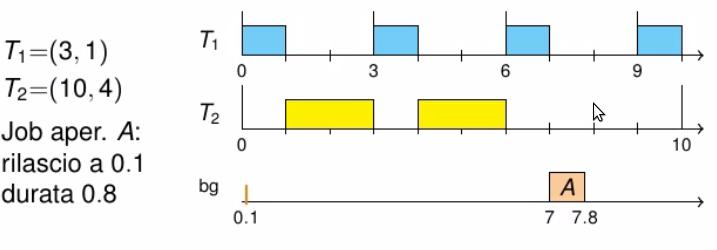
\includegraphics[scale=0.4]{immagini/image-009.jpg}
\end{figure}
\subsubsection{Schedulazione di job aperiodici soft RT interrupt-driven}
Esegui job aperiodici nel mo,mento in cui li rilasci, algortimo non è corretto ma è ottimo: job aperiodici finiscono nei tempi minimi, ma task periodici possono mancare le scadenze.\\
\begin{figure}[!h]
\centering
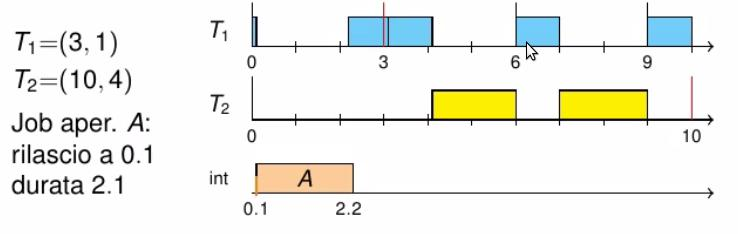
\includegraphics[scale=0.4]{immagini/image-010.jpg}
\end{figure}
\subsubsection{Schedualzione di job aperiodici soft RT con slack stealing}
Algoritmo esegue i job aperiodici in anticipo rispetto a quelli periodici finché c'è uno slack globale positivo.\\ È corretto perché i job periodici non perdono le scadenze. È ottimale, solo per job aperiodico in cima alla coda. Svantaggio è che tenere uno slack globale in uno scheduler priority divern è difficile.
Job aperiodico riprende quando lo slack torna positivo.\\
\begin{figure}[!h]
\centering
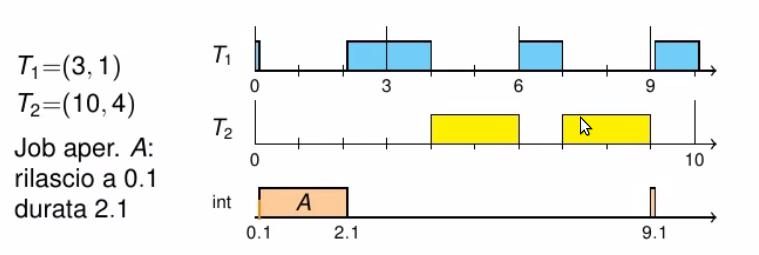
\includegraphics[scale=0.4]{immagini/image-011.jpg}
\end{figure}
\subsubsection{Schedulazione di job aperiodici soft RT con polling}
Algoritmo basato su polling, ovvero nel sys di task periodici introduco server di polling o poller, a cui do un certo periodo p$_{s}$ e tempo di esecuzione e$_{s}$ e gli do priorità massima,così da ridurre i tempi di risposta dei job aperiodici. Server controlla coda job aperiodici, se vuota si auto-sospende fino a prossimo tick, altrimenti esegue per al più
e$_{s}$ unità di tempo, per poi auto-sospendersi.\\ 
\begin{figure}[!h]
\centering
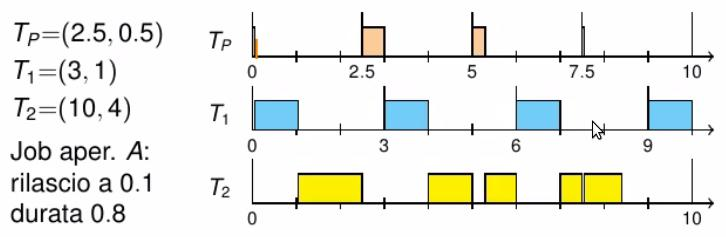
\includegraphics[scale=0.4]{immagini/image-012.jpg}
\end{figure}
È corretto se dimensiono il poller in modo tale che il suo fattore di utilizzazione non ecceda quello dell'algoritmo di schedulazione, è come aggiungere un task periodico che ha worst case pari ad e$_{s}$. \\ Non è ottimale, job aperiodico può arrivare subito dopo esecuzione del poller. Nell'esempio forse potevo anticipare l'esecuzione del job A senza far mancare le scadenze. Posso migliorare le capacità del server? Sì.
\subsubsection{Server periodici}
I server periodici sono una classe di task periodici aventi:
\begin{itemize}
\item periodo p$_{s}$
\item budget e$_{s}$
\item dimensione u$_{s}$ = $\frac{e_{s}}{p_{s}}$
\end{itemize}
Hanno due regole:
\begin{itemize}
\item regola di consumo che dice come il budget viene consumato
\item regola di rifornimento: come il budget viene ripristinato
\end{itemize}
Server di dice impegnato quando ha del lavoro da svolgere, ovvero la coda dei job aperiodici non è vuota, idle nel caso contrario. È eleggibile, pronto o schedulabile se è impegnato ed il suo budget è $>$ 0. Il poller può essere descritto come server periodico, è impegnato se la coda dei job non è vuota, la regola di consumo è che sottrae il tempo impiegato ad eseguire il job aperiodico dal budget; le coda dei job aperiodici è vuota il budget viene azzerato.\\ Budget rifornito del suo valore massimo e$_{s}$ all'inizio di ogni periodo p$_{s}$.
\subsection{Algoritmi a conservazione di banda}
Problema del server di polling è che se si svuota la coda, il server ha budget azzerato. Se subito dopo arriva un job che potrebbe essere subito  dal server non può farlo: questo comporta ritardo di esecuzione. VOlgio un algoritmo in cui un budget non venga azzerato se la coda è vuota, in modo da migliorare tempi di risposta se arrivano job aperiodici. Esistono molti algoritmi a conservazione di banda.3 di cui parleremo:
\begin{itemize}
\item Server procrastinabile
\item Server sporadico
\item Server a utilizzazione costante
\end{itemize}
Sono già molto sofisticati, usarne di più sofisticati comporterebbe overhead computazionale elevato. Questi algoritmi usati anche altrove, es gestione code di pacchetti.
\subsection{Server procrastinabile}
Server più semplice possibile. Devo definire le regole di consumo e riferimento, premesso che ho consumo p$_{s}$ e budget p$_{s}$. Regola di consumo: budget è decrementato di 1 per ogni unità di tempo in cui il server è in esecuzione (è proporzionale, quindi se è meno di 1 unità perdo meno di 1 unità). Non viene azzerato il budget se la coda dei job aperiodici è vuota.\\ Regola di rifornimento: ad ogni istante multiplo di p$_{s}$, il budget è impostato ad e$_{s}$. Nota bene: il budget non si accumula, quello che non spendo viene perso.\\
\begin{figure}[!h]
\centering
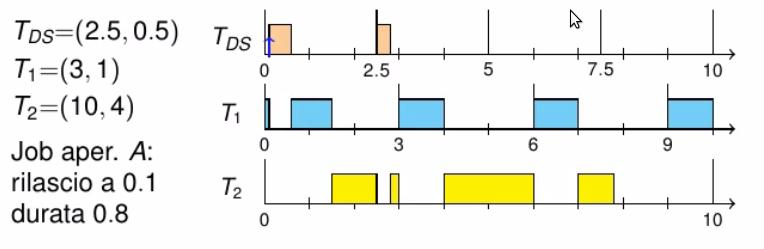
\includegraphics[scale=0.4]{immagini/image-013.jpg}
\end{figure}
stesso esempio di prima, all'istante 0 coda è vuota e quindi scheduler seleziona qualcun altro, quando a 0.1 arriva job aperiodico, questo interrompe job di T$_{1}$ ed esegue per 0.5 che è il budget massimo. Questo tipo di server minimizza tempo di risposta del job aperiodico. esempio: schedulazione a priorità fissa\\
\begin{figure}[!h]
\centering
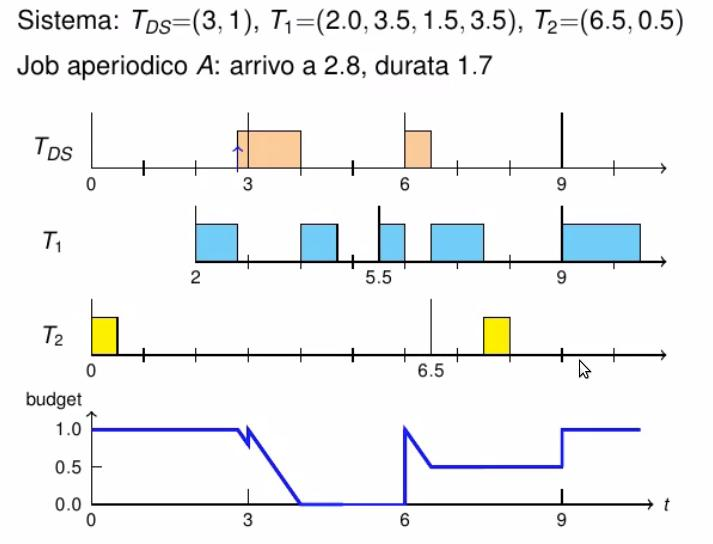
\includegraphics[scale=0.4]{immagini/image-014.jpg}
\end{figure}
\\All'inizio server non ha nulla da fare, va in esecuzione job di T$_{2}$, le cose cambiano quando all'istante 2.8 arriva il job aperiodico di durata 1.7, server ha priorità superiore, budget è positivo quindi è eleggibile e quindi esegue fino a 3. All'istante 3 cade il periodo del server, quindi budget è rifornito ad 1 ed esegue fino anche non finisce.Va eseguito altro, rimetto dentro il job di T$_{1}$, dopo di che non succede nulla: processore è idle anche se avrebbe qualcosa da fare, job aperiodico non è finito, ma algoritmo continua a non schedulare job. All'istante 6 termino job aperiodico e tutto procede. È vero che l'algoritmo cerca di anticipare esecuzione dei job aperiodici, ma non è perfetto. Non è ad esempio come un slack stealing, ho dei limiti: intervallo in cui processore è idle.\\ Posso fare la stessa schedulazione con EDF, in questo caso server non ha la priorità più grande: la priorità è data dalla scadenza assoluta che è data implicitamente dai periodi del server.Schedulazione simile a quella di prima, ci anche sono degli istanti in cui il processore è idle.\\ È possibile applicare condizioni di schedulabilità a sistemi a priorità fissa con server procrastinabile? La difficoltà è che il caso peggiore non è più vero, perché il server procrastinabile non ha un comportamento simile agli altri task periodici. Se il server è eleggibile e nessun task di priorità maggiore è in esecuzione viene subito eseguito, ma qui non appena arriva job aperiodico task diviene eleggibile, ma non so in che istante arriva il job: server con budget $>$ 0 può diventare eleggibile in qualunque momento. esempio: T$_{DS}$=(3,1.2), T$_{1}$=(3.5,1.5), r$_{1,c}$=10, r$_{A}$=10, e$_{A}$ $>$ 3, budget(10)=1.2, fase=2.2\\ All'istante 10 viene rilasciato job di T$_{1}$, ma all'istante 10 sto anche eseguendo job molto lungo aperiodico, questo job viene eseguito fino allo scadere del budget. Caso peggiore vuole che a 11.2 c'è scadenza del periodo del server, quindi budget è nuovamente incrementato, quindi esegue per un altro tempo e si azzera a 12.4, ma a 12.4 non c'è più abbastanza tempo per eseguire job di T$_{1}$. Assunzione non più vera: job arriva in un qualsiasi momento, configurazione è tale per cui job continua ad eseguire per un tempo più lungo di quello che doveva ed intacca job regolare.
\subsubsection{Istanti critici per server procrastinabili}
Sistema di task periodici indipendenti e interrompibili, e priorità fissa con D$_{i}$ $\leq$ p$_{i}$ ed un server procrastinabile (p$_{s}$, e$_{s}$) con priorità massima, un istante critico di un task T$_{i}$ si verifica all'istante t$_{0}$ se 
\begin{itemize}
\item a t$_{0}$ è rilasciato un job di tutti i task T$_{1}$,...,T$_{i}$
\item a t$_{0}$ il budget del server è e$_{s}$
\item a t$_{0}$ è rilasciato almeno un job aperiodico che impegna il server da t$_{0}$ in avanti
\item l'inizio del successivo periodo del server è t$_{0}$ + e$_{s}$
\end{itemize}
Nelle ipotesi del lemma, quanto tempo di processore occupa al massimo il server nell'intervallo (t$_{0}$, t]. Devo aggiungere questo tempo alla funzione di tempo necessario di T$_{i}$. Tempo totale: devo considerare anche il periodo troncato prima di t perché il server ha priorità massima, ho sicuro un e$_{s}$, poi ho e$_{s}$ per il numero di intervalli:
e$_{s}$ + $\lceil \frac{t-t_{0}-e_{s}}{p_s}\rceil \cdot e_s$.\\ Ora posso modificare la funzione di tempo necessario per tenere conto del server procrastinabile:\\ 
w$_{i}$(t) = e$_{i}$ + b$_{i}$ + e$_{s}$ + $\lceil \frac{t-t_{0}-e_{s}}{p_s}\rceil \cdot e_s$ + $\sum\limits_{k = 1}^{i-1}\lceil \frac{t}{p_{k}}\rceil \cdot e_k$ per 0 $<$ t $\leq$ p$_{i}$.\\ Il test controlla se w$_{i}$(t) $\leq$ t per i valori di t $\leq$ D$_{i}$ tali che t = h $\cdot$ p$_{k}$ oppure t = e$_{s}$ +  h $\cdot$ p$_{s}$, oppure t = D$_{i}$(h=0,1,...)\\ Stesso avviene per il test di schedulabilità generale:\\ j$\cdot$ e$_{i}$ + b$_{i}$ + e$_{s}$ + $\lceil \frac{t-t_{0}-e_{s}}{p_s}\rceil \cdot e_s$ + $\sum\limits_{k = 1}^{i-1}\lceil \frac{t}{p_{k}}\rceil \cdot e_k$ per 0 $<$ t $\leq$ p$_{i}$ per (j-1)$\cdot$ p$_{i}$ $<$ t $<$ w$_{i,j}$(t).\\ L'esempio nel caso precedente mostra che il task T$_{1}$ non è schedulabile.\\ Posso anche realizzare un sistema in cui server non ha priorità massima, condizione mi da risultato pessimista ma la condizione è solo sufficiente (può dare falsi negativi).
\subsubsection{Condizione di schedulabilità RM con server procrastinabile}
Teorema: un server procrastinabile con periodo p$_{s}$ e budget e$_{s}$ ed n task periodici indipendenti ed interrompibili , con p$_{i}$ = D$_{i}$ e tali che:\\ p$_{s}$ $<$ p$_{1}$ $<$... $<$ p$_{n}$ $<$ 2p$_{s}$ e p$_{n}$ $>$ p$_{s}$ + e$_{s}$ sono schedulabili con RM se l'utilizzazione totale è:\\
U$_{RM/DS}$(n) = $\frac{e_s}{p_s}$ + [$(\frac{e_s + 2p_s}{p_s +2e_s})^{\frac{1}{n}}$ -1]. Molto simile alla formula di Liu-Layland, facile verificare che se e$_{s}$ = 0, ottengo esattamente U$_{RM}$(n), ma ora $\lim_{x \to inf}$ U$_{RM/DS}$(n) = $\frac{e_s}{p_s}$ + ln($\frac{e_s + 2p_s}{p_s +2e_s}$).\\ Mi dice quanto è il carico massimo che posso dare al sistema quando c'è server procrastinabile in modo da garantire le scadenze, valgono però le ipotesi molto forti.\\ Se le condizioni non si verificano, bisogna effettuare analisi task per task:
\begin{itemize}
\item Server non ha alcuna influenza sui task con periodo minore di p$_{s}$
\item Server è schedulabile se lo è il corrispondente task periodico
\item Per i task di priorità inferiore devo prevedere che il server può bloccare per un tempo e$_{s}$ in più, aggiungo alla formula il tempo di blocco aggiuntivo:\\ $\sum\limits_{k = 1}^{i-1} \frac{e_k}{p_k}$ + $\frac{e_s}{p_s}$ + $\frac{e_s + b_i}{p_i}$ $\leq$ U$_{RM}$(i+1).\\ Aggiungo anche ritardo e$_{s}$ in più che è il primo intervallo, il ritardo dovuto al fatto che nell'istante critico per T$_{1}$ vengo rallento di un istante in più rispetto al tempo normale. Confronto al limite di Liu-Lyland per i+1 task perché includo anche il server.
\end{itemize}
\subsubsection{Condizione di schedulabilità di EDF con server procrastinabile}
Un task periodico T$_{i}$ in un sistema di n task indipendenti ed interrompibili è schedulabile con EDF insieme ad un server procrastinabile (p$_{s}$, e$_{s}$) se:\\ $\sum\limits_{k = 1}^{n} \frac{e_k}{min(D_k, p_k)}$ + $\frac{e_s}{p_s}$ $\cdot$ (1 + $\frac{p_s - e_s}{D_i}$) $\leq$ 1.\\ Dim: per D$_{k}$ $\leq$ p$_{k}$. Suppongo che un job di T$_{i}$ rilasciato a r$_{i}$ manca la scadenza a t; t' $<$ t è l'ultimo istante in cui il processore è idle o esegue un job a priorità inferiore. Ma allora r$_{i}$ $\geq$ t', questo significa che l'istante t in cui manco la scadenza assoluta meno t' è maggiore o uguale alla scadenza relativa. Ma quindi, invertendo: $\frac{1}{t-t'}$ $\leq$ $\frac{1}{D_i}$. Quando tempo viene rubato dal server procrastinabile tra t' e t: $e_{s}$ + $\lfloor \frac{t - t'- e_s}{p_s}\rfloor \cdot e_s$, la parte intera è inferiore perché se t cade nel mezzo vuol dire che il server procrastinabile avrà una scadenza che sarà dopo, la frazione va scartata in quanto non ruberà tempo.\\
\begin{figure}[!h]
\centering
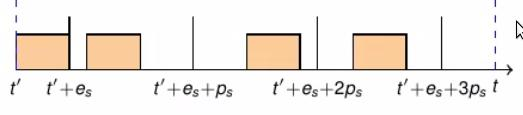
\includegraphics[scale=0.4]{immagini/image-015.jpg}
\end{figure}
Quindi t-t' $<$ $\sum\limits_{k=1}^{n} \frac{e_k}{p_k} \cdot (t-t')$ + $\frac{e_s}{p_s}$ $\cdot$ (t-t'-p$_s$-e$_{s}$). L'intervallo non è sufficiente a fare tutto il lavoro: il lavoro è eseguire tutti i job periodici, in più il tempo del server procrastinabile nell'intervallo t-t' ed in più +p$_{s}$ - e$_{s}$, togliendo la parte intera. Ma sto dicendo che la sommatoria + il resto è $>$ 1, ovvero se la condizione è $\leq$ 1 il task periodico rispetterà la scadenza.
\subsection{Server sporadici}
Un server procrastinabile può ritardare i task di priorità minore più di un task periodico con identici parametri. Vorrei avere un server con impatto su schedulabilità del sistema uguale a quello di un qualsiasi task periodico: server sporadico, shcedulabilità del sistema si studia semplicemente, ne esistono vari tipi: differenza sta nelle regole di consumo/rifornimento.
\subsubsection{Server sporadici in sistemi a priorità fissa}
Sistema di task periodici T a priorità fissa, ho un server sporadico T$_{s}$=(p$_{s}$, e$_{s}$), con priorità $\pi_{s}$. Definisco l'insieme T$_{H}$, che è l'insieme dei task con priorità maggiore di $\pi_{s}$.\\ Definisco l'intervallo totalmente occupato di un insieme di task:
\begin{itemize}
\item prima dell'intervallo tutti i job sono stati completati
\item all'inizio dell'intervallo viene rilasciato almeno un job
\item la fine dell'intervallo è il primo istante in cui tutti i job rilasciati entro l'intervallo sono completati
\end{itemize}
Definisco alcuni parametri e variabili:
\begin{itemize}
\item t$_{r}$: l'ultimo istante in cui è stato aumentato il budget, ovvero l'ultimo istante in cui è stata applicata la regola di rifornimento del server.
\item t$_{f}$, che è il primo istante dopo t$_{r}$ in cui il server è in esecuzione.
\item t$_{e}$ è invece una variabile che serve per indicare quando ci sarò il prossimo rifornimento, tipicamente sarà t$_{e}$ + $\pi_{s}$.
\item BEGIN: variabile che per ogni t, considera l'ultima sequenza di intervalli totalmente occupati contigui dei task T$_{H}$ iniziata prima di t. BEGIN è esattamente l'inizio del primo intervallo totalmente questa sequenza.
\item END è la fine, ma solo se la fine è precedente a t, altrimenti è $\infty$.
\end{itemize}
\subsubsection{Server sporadico semplice}
Regola di consumo: in ogni istante maggiore di t$_{r}$, il budget è decrementato di una unità per ogni unità di tempo se una delle seguenti condizioni è vera:
\begin{enumerate}
\item Il server è in esecuzione
\item Il server è stato in esecuzione dopo t$_{r}$ ed inoltre END $<$ t.
\end{enumerate}
Se le condizioni sono false, il budget si conserva. Il server consuma budget più in fretta del server procrastinabile, stiamo cercando di ridurre l'impatto che ha sui task di priorità inferiore.\\  Regole di rifornimento:
\begin{enumerate}
\item Ogni volta che faccio rifornimento, il budget è settato ad e$_{s}$, t$_{r}$ viene associato all'istante corrente
\item All'istante t$_{f}$:
\begin{itemize}
\item se END = t$_{f}$, allora associa a t$_{e}$ il max(t$_{r}$, BEGIN)
\item se END $<$ t$_{f}$, associa a t$_{e}$ il valore di t$_{f}$.
\end{itemize}
\item Il prossimo rifornimento sarà a t$_{e}$+p$_{s}$, ma con due eccezioni:
\begin{itemize}
\item se t$_{e}$+p$_{s}$ $<$ t$_{f}$, il budget sarà rifornito non appena esaurito
\item il budget sarà rifornito ad un certo momento t$_{b}$ $<$ t$_{e}$+p$_{s}$ se esiste un intervallo [t$_{i}$, t$_{b}$) in cui nessun task di T è eseguibile, ed un task di T comincia l'esecuzione a t$_{b}$
\end{itemize}
\end{enumerate}
Significato della regola di consumo 1: nessun job del server esegue per un tempo maggiore di e$_{s}$ in un periodo p$_{s}$\\ Significato di C2: il server conserva budget se un task di T$_{H}$ è eseguile oppure il server non ha mai eseguito t$_{r}$; altrimenti il budget è consumato.\\ Significato di R2: se nell'intervallo (t$_{r}$, t$_{f}$) sono stati sempre in esecuzione task di T$_{H}$, il prossimo rifornimento sarà a t$_{r}$+p$_{s}$. Ma se questo non è vero il prossimo rifornimento sarà a t$_{e}$+p$_{s}$ dove t$_{e}$ è l'ultimo istante di (t$_{r}$, t$_{f}$] in cui non esegue un task di T$_{H}$.\\ Significato di R3a: il job del server ha atteso per più di p$_{s}$ unità di tempo prima di iniziare l'esecuzione, quindi il job continua nel prossimo periodo (serve il test di schedulabilità generale).\\ R3b: il budget è rifornito nell'ostante iniziale di ogni intervallo totalmente occupato di T. \\ esempio di schedulazione RM con server sporadico semplice:\\
\begin{figure}[!h]
\centering
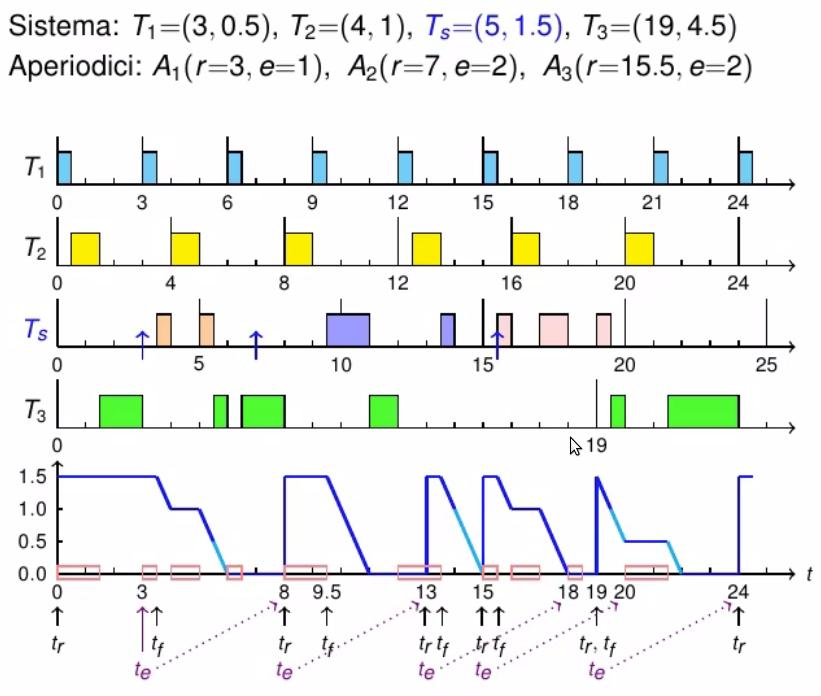
\includegraphics[scale=0.4]{immagini/image-016.jpg}
\end{figure}
Da 3.5 comincio T$_{f}$ e consumo il budget, ma ora devo anche capire t$_{e}$, che qui è 3. Questo mi dice anche quando sarà il prossimo rifornimento, che sarà ad 8 (3+5). All'istante 5.5 termina il job aperiodico, e qui lo scheduler da il controllo al job di T$_{3}$, ma il budget continua ad essere consumato fino a diventare 0: non sono più nelle condizioni in cui il budget si preserva, e qui sta eseguendo un job con priorità minore del server. All'istante 7 arriva il 2° job aperiodico ma non posso eseguirlo perché il budget è 0, quindi devo aspettare 8. A 9.5 termina l'intervallo totalmente occupato, quindi posso eseguire job aperiodici.
\subsubsection{Server sporadico background}
Variante del server sporadico (ne esistono di verse via via sempre più costose da implementare). Ogni volta che nessun job periodico è eseguibile, il server esegue un job aperiodico.\\ Regola di consumo è identica a quella del server sporadico semplice, tranne che se nessun task periodico è eseguibile il budget è uguale a e$_{s}$. \\ regola di consumo è uguale tranne che per R3b: il budget è ripristinato all'inizio di ogni intervallo in cui nessun task periodico è eseguibile; t$_{r}$ (ed eventualmente t$_{f}$) è la fine dell'intervallo.\\ Conviene sempre implementare questo server, perché questo tende ad abbassare il tempi di risposta dei job aperiodici, l'unico caso in cui non conviene usarlo è quando si utilizzano più server sporadici per differenti tipi di job aperiodici.\\ esempio precedente:\\
\begin{figure}[!h]
\centering
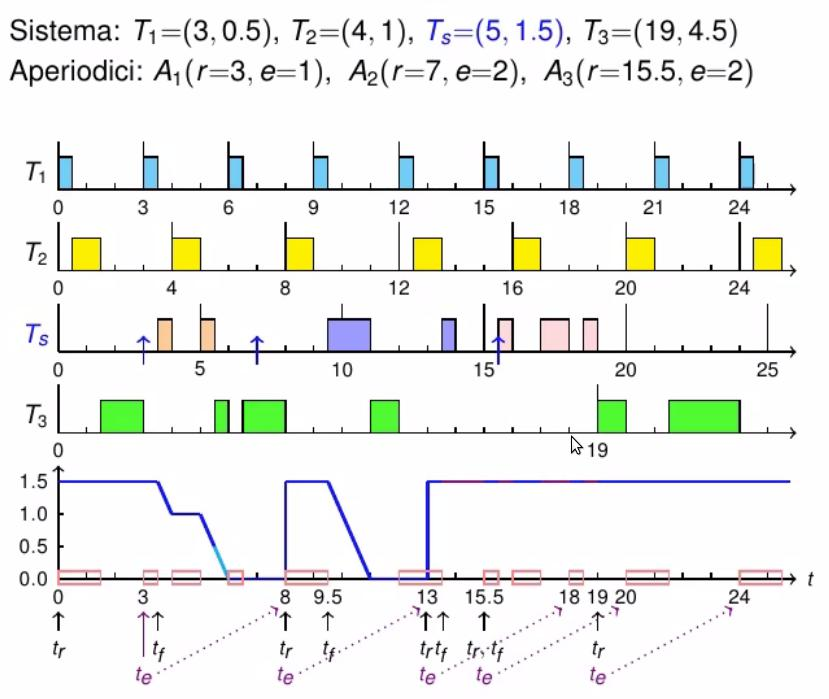
\includegraphics[scale=0.4]{immagini/image-017.jpg}
\end{figure} 
Da un certo punto in poi budget rimane sempre al valore massimo, per un motivo o per un altro.
\subsection{Constant Bandwidth server}
Server inventato da L. Abeni e G. Buttazzo (1998). Server abbastanza recente, importante per diversi motivi:
\begin{itemize}
\item Server abbastanza facile da integrare in uno scheduler a priorità fissa a livello di job
\item Schedulazione di job aperiodici con i vantaggi di EDF rispetto a RM/DM
\item server è work conserving: non lascio mai processore idle se c'è almeno un job da eseguire.
\item occupazione del processore non supera mai una frazione di tempo predefinita: permette di isolare il comportamento del server dal comportamento dei task aperiodici
\end{itemize}
Caratteristiche:
\begin{itemize}
\item periodo p$_{s}$
\item budget massimo e$_{s}$
\item budget corrente c$_{s}$
\item scadenza assoluta d$_{s}$: questo perché il server va schedulato in un algoritmo di tipo EDF, devo confrontare la priorità con quella degli altri task che è basato su scadenza assoluta.
\end{itemize}
Il rapporto u$_{s}$ = $\frac{e_s}{p_s}$ è la bandwidth del server.\\ Il server CBS viene schedulato con EDF insieme agli altri task periodici considerando la scadenza assoluta corrente d$_{s}$.\\ Un sistema di task periodici ed un server CBS sono schedulabili con EDF se U$_{T}$ + u$_{s}$ $\leq$ 1.\\ Funzionamento del server:\\
\begin{itemize}
\item Regola di aggiornamento della scadenza:
\begin{itemize}
\item inizialmente d$_{s}$ = 0
\item non appena budget corrente si azzera, la scadenza diviene pari a d$_{s}$+p$_{s}$, la priorità viene diminuita in modo da dare spazio agli altri task del sistema
\item Se ad un certi istante t viene rilasciato job aperiodico ed il server non è impegnato (la coda dei job aperiodici è vuota) , vado a verificare se c$_{s}$ $\geq$ (d$_{s}$-t) $\cdot$ u$_{s}$, perché se questo avviene rischio di prendere più tempo del processore del dovuto e quindi setto d$_{s}$ a t+p$_{s}$.
\end{itemize}
\item Regola di rifornimento e di consumo:
\begin{itemize}
\item all'inizio imposto il valore di c$_{s}$ ad e$_{s}$
\item c$_{s}$ viene decrementato proporzionalmente all'esecuzione dei job periodici del server.
\item se c$_{s}$ di azzera, c$_{s}$ viene rifornito ad e$_{s}$ immediatamente
\end{itemize}
Non esiste mai un intervallo di tempo $>$ 0 in cui il server ha un budget nullo.
\end{itemize}
esempio EDF con server CBS:
\begin{figure}[!h]
\centering
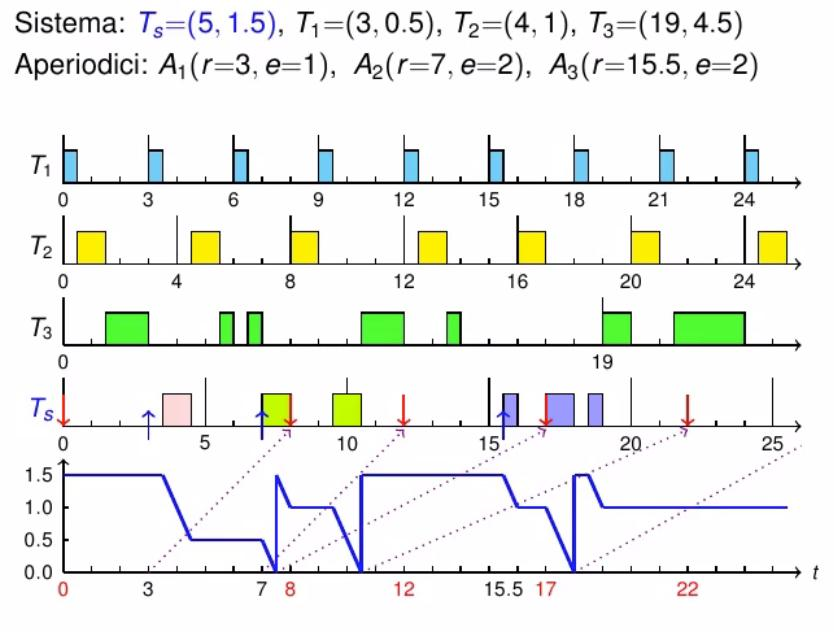
\includegraphics[scale=0.4]{immagini/image-018.jpg}
\end{figure}
\subsection{Schedulabilità di job aperiodici hard real-time}
Concetto di densità del job aperiodico con istante di rilascio r e tempo massimo di esecuzione e e scadenza la sua densità è: $\frac{e}{d-r}$.\\ Vale questo teorema: Un sistema di job aperiodici, indipendenti e interrompibili è schedulabile con EDF se la densità totale di tutti i job attivi (nell'intervallo tra rilascio e scadenza) è in ogni istante $\leq$ 1.\\ In ogni istante di tempo la densità totale di tutti i job rilasciati e non ancora conclusi deve essere $\leq$ 1; è una condizione sufficiente, teorema permette di realizzare anche un test di accettazione. Dim: un job manca la scadenza a t, t' è l'ultimo momento in cui il processore non ha eseguito un job con scadenza $\leq$ t $\Rightarrow$ $\sum\limits_{i} e_i$ $>$ t-t'. Partiziono l'intervallo fra (t',t] in (t$_{1}$,t$_{2}$],(t$_{2}$,t$_{3}$].... dove t$_{k}$ è l'istante di rilascio o scadenza per qualche job, in ciascuno dei quali l'insieme dei job attivi è differenze. Considero X$_{k}$ l'insieme dei job attivi in (t$_{k}$,t$_{k+1}$] e $\Delta_k$ la loro densità:\\ $\sum\limits_{i} e_i$ =  $\sum\limits_{j = 1}^{l} (t_{j+1} - t_j)$ $\cdot$ $\sum\limits_{J_{k} \in X_{i}} \frac{e_k}{d_k - r_k}$ $\leq$ $\sum\limits_{j = 1}^{l} \Delta_{j}(t_{j+1} - t_j)$ $\leq$ t-t'. Vedo la somma di e$_{i}$ come la densità per quell'intervallo moltiplicata per la lunghezza dell'intervallo. Ma il risultato è in contraddizione col fatto che qualcuno ha mancato la scadenza. esempio: \\
Considero job aperiodici J$_{1}$=(r=0, e=1,d=2), J$_{2}$=(r=0.5, e=1,d=2.5), J$_{3}$=(r=1, e=1,d=3)\\
\begin{table}
\begin{tabular}{||c c c||}
\hline\hline
intervalli & job attivi & densità\\
\hline
(0, 0.5] & J$_{1}$ & 0.5\\
\hline
(0.5,1] & J$_{1}$J$_{2}$ & 1.0\\
\hline
(1,2] & J$_{1}$J$_{2}$J$_{3}$ & 1.5\\
\hline
(2,2.5] & J$_{2}$J$_{3}$ & 1.0\\
\hline
(2.5,3] & J$_{3}$ & 0.5
\end{tabular}
\end{table}
Nell'intervallo (1,2] la densità totale è $>$ 1, quindi il teorema non si applica. Schedulabilità con EDF? Sì, il teorema è solo sufficiente: metto J$_{1}$ in (0,1], J$_{2}$ in (1,2] e J$_{3}$ in (2,3] ed ottengo la mia schedulazione.
\chapter{Controllo d'accesso alle risorse condivise}
\section{Controllo d'accesso alle risorse condivise}
Sono partito da modello di carico nel sistema in cui tutti i job erano semplificati, task rilasciavano i job in maniera regolare e tutti i job erano indipendenti ed interrompibili. Mano a mano rilassato queste ipotesi, estendendo il modello. Continuo ad avere singolo processore, sciolgo vincolo di indipendenza dei job nel senso delle risorse condivise. Risorse condivise: accedervi significa vietare a qualunque altro job l'accesso finché il lavoro non è concluso.\\ Nel modello dico che esistono una serie di risorse riciclabili R$_{1}$, R$_{2}$,...., R$_{\rho}$ e ciascuna risorsa R$_{i}$ ha $\nu_{i}$ unità di risorsa indistinguibili assegnabili, non posso assegnare la stessa unità di risorsa a più job ma più job può acquisire più unità di risorsa.\\ Se R$_{i}$ ha un numero $\infty$ unità di risorsa non vale la pena considerarla nel modello,  considero quindi $\nu_{i}$ sempre finito.\\ esempi: semafori, mutex, spin lock, stampanti erc..., si parla di risorse passive: l'unica cosa che conta è che siano disponibili, non sono importanti le loro caratteristiche interne.\\ Come modello una risorsa R che può essere utilizzata da un numero finito di job n $>$ 1: R ha $\nu$ unità esclusive, ovvero nessun job può ottenere più di 1 unità. \\ Come modello invece risorsa R che ha una intrinseca dimensione finita (es una memoria): capisco qual'è l'unità di assegnazione della memoria, ad esempio un pagina di memoria, e faccio corrispondere a $\nu$ il più piccolo blocco di risorsa assegnabile.
\subsection{Richieste e rilasci di risorse}
Un jbo che deve acquisire un certo n° $\eta$ di unità della risorsa R$_{i}$ procede ad effettuare la richiesta L(R$_{i}$, $\eta$). La richiesta è atomica: o ottiene tutte  le $\eta$ unità, altrimenti il job è bloccato (la sua esecuzione è sospesa).Termine blocco è giustificato nel contesto: se non posso ottenere la risorsa, vuol dire che un job a priorità minore di me ha la risorsa. Quando job non ha più bisogno della risorsa fa un rilascio U(R$_{i}$, $\eta$).\\ Spesso il controllo di accesso è affidato a primitive software di tipo lock/unlock. Spesso la risorsa R$_{i}$ ha una sola unità disponibile ($\nu_i$ = 1), abbrevio quindi con L(R$_{i}$) ed U(R$_{i}$). È una semplificazione, ama algoritmi che studio sono facilmente adattabili ad un situazione con $\eta$ variabile.\\ Conflitto di risorse: due job hanno un conflitto di risorse se potenzialmente possono chiedere una risorsa dello stesso tipo. Due job si contendono una risorsa se uno dei due richiede una unità di risorsa che è già posseduta dall'altro job.
\subsection{Sezioni critiche}
Si definisce sezione critica un segmento di esecuzione di jon che inizia con L(R$_{i}$, $\eta$) e termina con U(R$_{i}$, $\eta$). Le richieste di risorse di un job possono essere annidate, ma assumiamo che i rilasci sono sempre LIFO.\\ Una sezione critica non contenuta in alcun'altra sezione critica è detta esterna.\\ La notazione [R$_{1}$, $\eta_1$;e$_{1}$[R$_{2}$,$\eta_2$;e$_{2}$]] corrisponde a:\\ L(R$_{i}$, $\eta_1$) L(R$_{2}$, $\eta_2$) U(R$_{2}$, $\eta_2$) U(R$_{1}$, $\eta_1$) rispettivamente la lunghezza di e$_{2}$ è contenuta nella la lunghezza di e$_{1}$ (ovvero nella regione critica di R$_{1}$ viene fatta la richiesta di R$_{2}$). Quando un certo job richiede una certa risorsa? Non c'è l'indicazione, ragiono sul worst case. esempio:\\
schedulazione con EDF con una unità di risorsa (notazione: freccia bassa è richiesta di risorsa, freccia alta è rilascio).\\
\begin{figure}[!h]
\centering
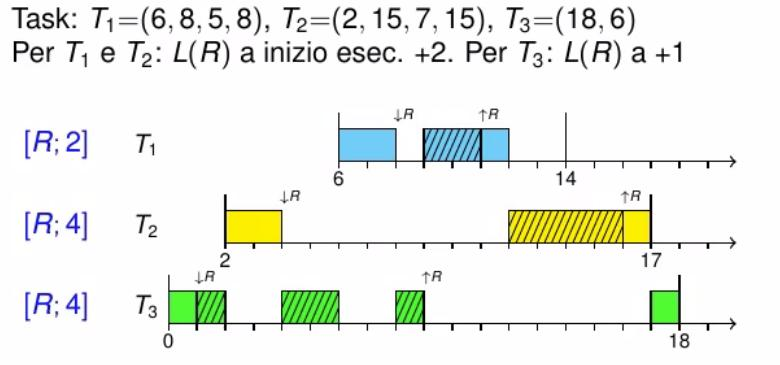
\includegraphics[scale=0.4]{immagini/image-019.jpg}
\end{figure}
Le inversioni di priorità causata dal possedere la risorsa causa anomalie di schedulazione: se ad esempio riduco la durata della regione critica d T$_{3}$, quindi apparentemente i job di priorità più alta dovrebbero essere favoriti, ma non è così:\\ 
\begin{figure}[!h]
\centering
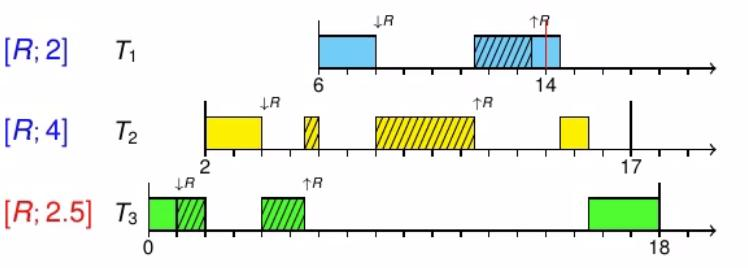
\includegraphics[scale=0.4]{immagini/image-020.jpg}
\end{figure}
quando job di T$_{3}$ rilascia la risorsa, il job di T$_{1}$ non è ancora stato rilasciato e quindi entra job di T$_{2}$, quindi T$_{1}$ otterrà la ricorsa troppo tardi. Le inversioni di priorità possono causare anomalie di schedulazione, devo tenerne conto nell'analisi di schedulabilità.
\subsection{Controllo d'accesso alle risorse condivise}
Algoritmi per il controllo di accesso sono necessari:
\begin{itemize}
\item Le inversioni di priorità devono essere controllate, altrimenti sarebbero arbitrariamente lunghe.esempio: J$_{3}$ acquisisce risorsa e poi viene bloccato da J$_{1}$ che vuole acquisire risorsa. Ma ora entra job di J$_{2}$ e può essere deciso dallo scheduler di metterlo nel processore, perché a priorità maggiore di J$_{3}$: J$_{2}$ rallenta sia J$_{3}$ che J$_{1}$. Il ritardo che J$_{3}$ infligge a J$_{1}$ non è solo la lunghezza della regione critica fra J$_{3}$ e J$_{1}$ va misurata nel momento in cui nessuno interrompe J$_{3}$, se ci sono processi che interrompono J$_{2}$ a priorità maggiore che prendono il posto di J$_{3}$ non so quanto sarà lungo il blocco di J$_{1}$ (posso avere molteplici job nel mezzo che rallentano). Questo fenomeno si chiama inversione di priorità non controllata.
\item Deadlock: altro grave problema. J$_{2}$ chiede R$_{1}$, J$_{1}$ chiede R$_{2}$. A quel punto J$_{1}$ chiede R$_{1}$ ma è bloccato, J$_{2}$ continua ed ad un certo punto richiede R$_{2}$. Sono in una situazione di deadlock.
\end{itemize}
\subsubsection{Grafi di attesa}
Mutua relazione tra job e risorse è modellabile con grafi di attesa: i nodi dono i job, altri nodi le risorse. Un arco da un nodo di tipo risorsa ad un di tipo job indica che il job ha allocato un certo n° di unità della risorsa. Il viceversa indica che job ha richiesto un certo numero di unità della risorsa ma questa non può essere soddisfatta. Un ciclo del grafo rappresenta un deadlock:\\
\begin{figure}[!h]
\centering
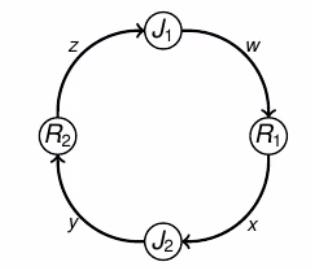
\includegraphics[scale=0.4]{immagini/image-021.jpg}
\end{figure}
\subsection{Protocollo NPCS}
Il più semplice protocollo di accesso alle risorse condivise, Nonpreemptive Critcial Section: un job avente una risorsa assegnata non può essere interrotto.\\ Questo risolve tutti i problemi, posso avere deadlock? No, solo a condizione che il job non si auto-sospenda quando ha la risorsa: se job ottiene risorsa e non può essere interrotto non può esserci deadlock, job di priorità superiore non potrà richiedere altra risorsa perché non potrà andare in esecuzione. Se job si auto-sospende tutto il discorso cade: processore è libero e qualcuno può essere schedulato, richiedere una risorsa ed alla fine causare un deadlock.\\ esempio precedente,  schedulazione con NPCS:\\
\begin{figure}[!h]
\centering
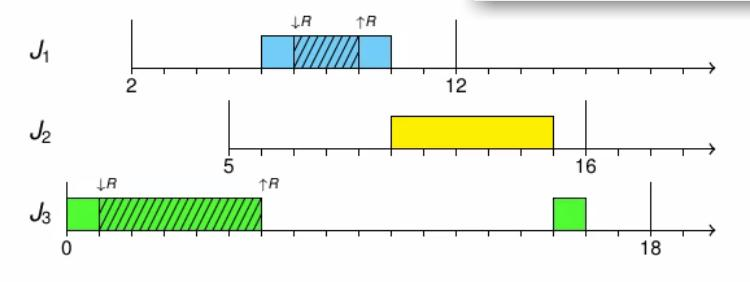
\includegraphics[scale=0.4]{immagini/image-022.jpg}
\end{figure}
Non ci sono deadlock e non c'è inversione di priorità incontrollata: al massimo J$_{1}$ sarà bloccato da J$_{3}$ per una durata pari alla regione critica.
\subsubsection{Tempo di blocco per conflitto di risorse}
Sia b$_{i}$(rc) il tempo di blocco dovuto ad un conflitto di risorse. Per NPCS con task a priorità fissa T$_{1}$,....,T$_{n}$:\\
b$_{i}$(rc) = $\underset{i+1 \leq k \leq n}{max}$(c$_{k}$), dove c$_{k}$ è il tempo di esecuzione della più lunga sezione critica di T$_{k}$. Misuro il ritardo che subisce T$_{i}$, i job di priorità superiore non mi danno blocchi, se io voglio una risorsa e la trovo bloccata è per via di job a priorità minore, quelli a priorità superiore non mi fanno neanche entrare nel processore; questo in un modello a singolo processore e senza auto-sospensione.\\ Potrei subire un ritardo perché uno dei job a priorità inferiore alla mia è dentro la regione critica e quindi non può essere interrotto secondo NPCS.\\ Blocco per conflitto di risorse in NPCS è dovuto al fatto che un job a priorità inferiore è dentro la sezione critica.\\ Formula per b$_{i}$(cs) con schedulazione EDF, teorema di Baker: un job J$_{i}$ può essere bloccato da J$_{j}$ solo se d$_{i}$ $<$ d$_{j}$ e r$_{i}$ $>$ r$_{j}$, ossia D$_{i}$ $<$ D$_{j}$.\\ Quindi b$_{i}$(rc) = max\{c$_{k}$: k tale che D$_{k}$ $>$ D$_{i}$\}.\\ Limite del protocollo NPCS: un job può essere bloccato da un job a priorità inferiore anche quanto non ci sono contese o conflitti su alcune risorse. Svantaggioso, quindi si cerca di evitar questo protocollo. D'altra parte, il protocollo è molto diffuso perché è semplice da implementare, non richiede dati sull'uso delle risorse dei job e può essere usato sia per sistemi a priorità fissa che dinamica.
\subsection{Protocollo priority-inheritance}
Protocollo adatto ad ogni scheduler priority-driven, non si basa sui tempi di esecuzione dei job e riesce ad evitare il fenomeno dell'inversione di priorità incontrollata.\\ Idea: cambiare le priorità se esistono delle contese sulle risorse per evitare che un job blocca un altro job di priorità più alta sia rallentato da job di priorità intermedi fra i due. esempio di prima: quando J$_{1}$ richiede la risorsa, poi J$_{3}$ torna normalmente in esecuzione, poi arriva J$_{2}$ che rallenterebbe J$_{3}$, ma ora il fatto che J$_{3}$ sta bloccando J$_{1}$ al sua priorità sarà innalzata fino a quella di J$_{1}$. In questo modo evito che si possano inserire job di priorità intermedia.\\ In pratica: i job sono schedulati in modo interrompibile secondo la loro priorità corrente. inizialmente la priorità corrente $\pi$(t) di un job J rilasciato al tempo t è quella assegnata dall'algoritmo di schedulazione.\\ Quando un job J richiede una risorsa R al tempo t:
\begin{itemize}
\item Se R è disponibile, R vine assegnata a J
\item Se R non è disponibile, J è sospeso (bloccato)
\end{itemize}
Quando un job J viene bloccato a causa di una contesa su una risorsa R, il job J$_{l}$ che blocca J eredita la priorità corrente $\pi$(t)  di J finché non rilascia R; a quel punto, la priorità corrente di J$_{l}$ torna ad essere la priorità $\pi_{l}$(t') che aveva al momento t' in cui aveva acquisito la risorsa R.\\ esempio: schedulazione a priorità fissa con priority-inheritance, qui supponiamo che la risorsa venga chiesta dopo un'unità di tempo dal rilascio.\\
\begin{figure}[!h]
\centering
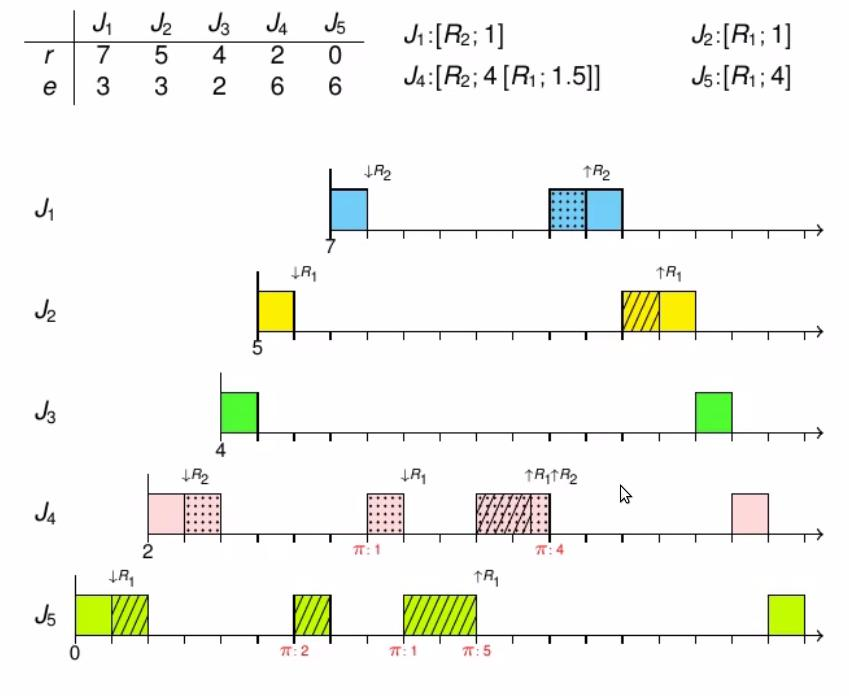
\includegraphics[scale=0.4]{immagini/image-023.jpg}
\end{figure}
Limiti:
\begin{itemize}
\item Non evita i deadlock
\item Introduce nuovi casi di blocco: un job a priorità corrente $\pi$(t) può bloccare ogni job con priorità assegnata minore di $\pi$(t).
\item Non riduce i tempi di blocco dovuti ai conflitti sulle risorse al minimo teorico possibile. esempio: ho un job a priorità alta: il job ha sotto di se molti job a priorità inferiore, usa molte risorse annidate. Se tutte le risorse sono assegnate: se accede ad un certo numero v di risorse ed ha conflitti con k job di priorità inferiore assegnata può bloccare per un min(k,v) volte.\\ Devo dimensionare il sistema in modo molto pessimista
\end{itemize}
\subsection{Protocollo priority-ceiling}
Adatto a scheduler con priorità fissa.È basato sulle richieste di risorse dei job prefissati, evita inoltre tutti e due i problemi.\\ Idea: associare ad ogni risorsa R il valore priority ceiling $\lceil\rceil$(R) pari alla massima priorità dei job che fanno uso di R. Dato che sa quale task userà quale risorsa, ad ogni risorsa è possibile associare il priority ceiling. Inoltre, il protocollo definisce il current priority ceiling $\lceil\rceil$'(R) che è apri a:
\begin{itemize}
\item La massima priorità $\lceil\rceil$(R) fra tutte le risorse del sistema correntemente in uso al tempo t
\item al valore convenzionale $\Omega$ di priorità  inferiore a quella di qualunque task se nessuna risorsa è in uso.
\end{itemize}
Confrontando le priorità, $\pi$(t) $>$ $\pi'$(t) significa che $\pi$(t) ha maggiore priorità di $\pi'$(t); così se a valore inferiore corrisponde priorità superiore, $\pi$(t) = 1 e $\pi'$(t) = 2 implica che $\pi$(t) $>$ $\pi'$(t).\\ Regola di schedulazione: job schedulati in modo interrompibile secondo la loro priorità corrente.\\ Se al tempo t un job J con una certa priorità corrente $\pi$(t) richiede una risorsa R, R è allocata a J sole se è disponibile d inoltre:
\begin{itemize}
\item $\pi$(t) $>$ $\lceil\rceil$(t)
\item J possiede una risorsa il cui priority ceiling è uguale a $\lceil\rceil'$(t)
\item altrimenti J è bloccato.
\end{itemize}
Se J$_{l}$ blocca J, J$_{l}$ eredità la priorità corrente $\pi$(t) di J finché J$_{l}$ non rilascia l'ultima risorsa R tale che $\lceil\rceil$(R) $\geq$ $\pi$(t); a quel punto la priorità di J$_{l}$ torna ad essere la priorità $\pi_{l}$(t') che aveva al momento t' in cui aveva acquisito la risorsa R.\\ esempio:\\
\begin{figure}[!h]
\centering
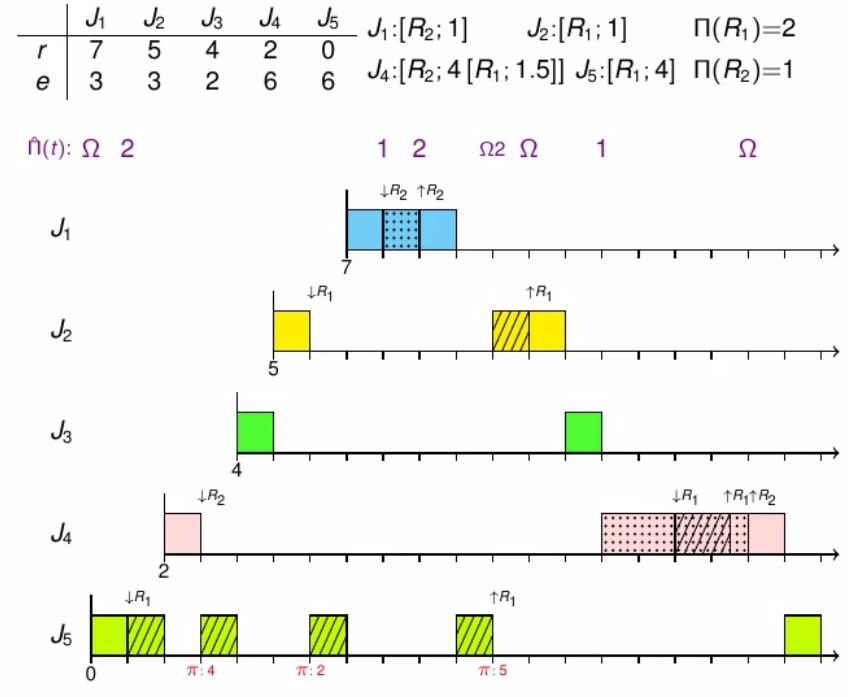
\includegraphics[scale=0.4]{immagini/image-024.jpg}
\end{figure}
Stabilisco prima i priority ceiling delle risorse. Ho un blocco: il motivo per cui J$_{4}$ non può continuare perché è bloccato da J$_{5}$, quindi J$_{5}$ eredita la priorità di J$_{4}$.\\ In quanti casi diversi un job J$_{l}$ può bloccare un job J$_{h}$ con priorità $\pi{l}$ $<$ $\pi{h}$:
\begin{itemize}
\item Blocco diretto: J$_{h}$ richiede una risorsa R assegnata a J$_{l}$.
\item Blocco dovuto a priority-inheritance: la priorità corrente di J$_{l}$ è maggiore di quella di J$_{h}$, perché J$_{l}$ sta bloccando direttamente un job che ha priorità maggiore di J$_{h}$.
\item Blocco dovuto al priority ceiling (o avoidance blocking): J$_{h}$ ha richiesto una risorsa R ma J$_{l}$ possiede un'altra risorsa R' tale che $\lceil\rceil$(R') $\geq$ $\pi_{h}$.
\end{itemize}
I deadlock possono essere evitati se tutti i job acquisiscono le risorse annidate rispettando un unico ordinamento globale delle risorse; metodo principale usato nei sistemi operativi.\\ I priority ceiling non definiscono un ordinamento globale delle risorse, bensì parziale ma che basta ad evitare i deadlock. esempio:\\
\begin{figure}[!h]
\centering
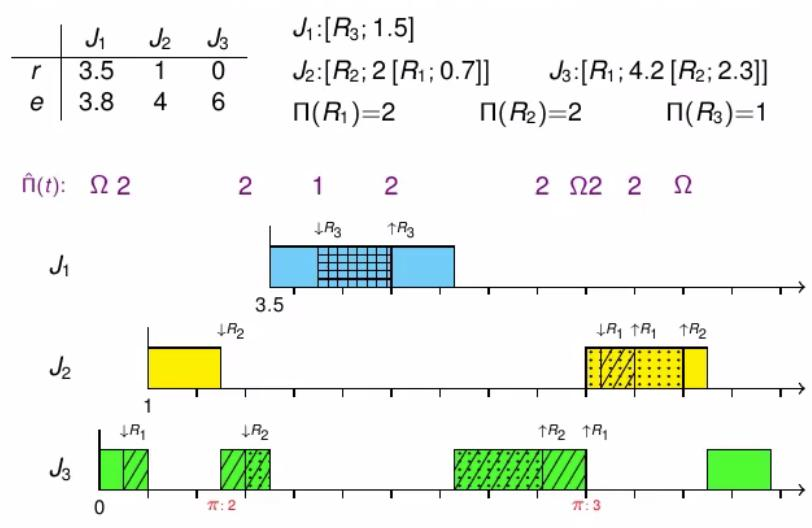
\includegraphics[scale=0.4]{immagini/image-025.jpg}
\end{figure}
Sono esposto ad un deadlock, ma con priority ceiling non avverrà: al tempo 2.5 J$_{2}$ richiede R$_{2}$, ma la richiesta viene rifiutata anche se R$_{2}$ è libera, così si evita un possibile deadlock con J$_{3}$. I job con priorità corrente maggiore di $\lceil\rceil'$(t) possono acquisire risorse sezna rischiare deadlock con le risorse già assegnate.\\ Posso avere molti job e risorse: ho J$_{1}$, che usa R$_{1}$,R$_{2}$, poi ho J$_{2}$ che usa R$_{3}$,R$_{4}$, userà anche R$_{1}$,R$_{2}$ ma non è un problema, perché il priority ceiling di R$_{1}$,R$_{2}$ è quelli di J$_{1}$ e così via per i vari livelli:\\
$\lceil\rceil$(R$_{1}$) = $\lceil\rceil$(R$_{2}$) = $\pi_{1}$\\
$\lceil\rceil$(R$_{3}$) = $\lceil\rceil$(R$_{4}$) = $\pi_{2}$.
e così via \\ Suppongo che $\lceil\rceil'$(t$_{0}$) sia ad un certo livello $\pi_{k}$: questo vuol dire che sono assegnate nel sistema solo risorse al di sotto di questo livello. Se al tempo t$_{0}$ un job richiede un risorsa e la sua priorità $\pi_{J}$(t$_{0}$) $>$ $\lceil\rceil'$(t$_{0}$):
\begin{itemize}
\item J non richiederà mai alcuna risorsa già assegnata al tempo t$_{0}$. Quindi non avrò nessun deadlock con le risorse già assegnate
\item Nessun job con priorità maggiore di $\pi_{j}$(t$_{0}$) chiederà alcuna risorsa già assegnata la tempo t$_{0}$ , quindi nessun job che già possiede una risorsa al tempo t$_{0}$ portà interrompere J e richiedere R.
\end{itemize}
Il risultato è che il protocollo priority-ceiling evita i deadlock.
\subsubsection{Proprietà del protocollo priority-ceiling}
Come visto sopra:
\begin{itemize}
\item al tempo t un job possiede tutte le risorse assegnate aventi priority ceiling uguale a $\lceil\rceil'$(t).
\item se un job sta per ottenere un risorsa $\pi$(t) $>$ $\lceil\rceil'$(t), nessun job di priorità uguale o superiore ha richiesto o richiederà le risorse già assegnate
\item Se un job sta per ottenere una risorsa $\pi$(t) = $\lceil\rceil'$(t), il job è il possessore di tutte le risorse assegnate aventi priority ceiling uguale a $\lceil\rceil'$(t).
\item i deadlock sono dunque evitati: priorità assegnate all risorse definiscono in un certo modo un ordinamento non totale tra le risorse.
\end{itemize}
Se al tempo t$_{0}$ un job J richiede una risorsa R e $\pi$(t$_{0}$) $>$ $\lceil\rceil'$(t): 
\begin{itemize}
\item J non richiederà mai alcuna risorsa già assegnata aò tempo t$_{0}$
\item Nessun job a priorità $\geq$ $\pi$(t${0}$) chiederà una risorsa già assegnata al tempo t$_{0}$.
\end{itemize}
Quindi priority ceiling evita i deadlock.\\ Non basta questa proprietà per giustificare la complessità di priority ceiling: basterebbe programmare bene i job nel sistema per evitare i deadlock.\\ In priority-ceiling, ho 3 blocchi possibili: blocco diretto, priority-inheritance, priority-ceiling.\\ C'è un teorema:\\ utilizzando il protocollo priority-ceiling un job può essere bloccato al massimo per la durata di una sezione critica.Teorema vuol dire che su un job subisce blocco a causa di una risorsa condivisa lo farà una volta sola, non subirà blocchi consecutivi. Inoltre blocco non sarà per un tempo costituito da annidamento di diverse sezioni critiche, ma per un tempo pari a solo la durata di una sezione critica.2 proprietà:
\begin{itemize}
\item Se un job viene bloccato, è bloccato da un solo job
\item Non esiste blocco transitivo: non si verifica mai il caso J$_{3}$ blocca J$_{2}$ e J$_{2}$ blocca J$_{1}$.
\end{itemize}
Unicità del job bloccante:\\ ho 3 job di priorità variabili.
\begin{figure}[!h]
\centering
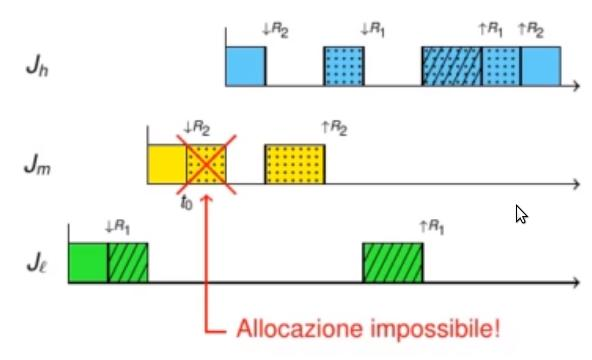
\includegraphics[scale=0.4]{immagini/image-026.jpg}
\end{figure}
J$_{h}$ è bloccato sia da J$_{m}$ che da J$_{l}$. Perché non può avvenire in priority ceiling:\\ $\pi_{h}$ $>$ $\pi_{m}$ $>$ $\pi_{l}$ $\Rightarrow$ $\lceil\rceil$(R$_{1}$) $\geq$ $\pi_{h}$ e $\lceil1rceil$(R$_{2}$) $\geq$ $\pi_{h}$.\\ Ora: $\lceil\rceil'$(t$_{0}$) $\geq$ $\lceil\rceil$(R$_{1}$) $\geq$ $\pi_{h}$. Il requisito per l'allocazione a t$_{0}$ deve essere $\pi_{m}$ $>$ $\lceil\rceil$(R$_{1}$) $\geq$ $\pi_{h}$. Ma questo non è verificato e quindi il priority ceiling nega l'assegnazione della risorsa a J$_{m}$.\\ Se J$_{m}$ acquisisce una risorsa a t$_{0}$, nessun job con priorità maggiore o uguale può richiedete una risorsa già in uso a t$_{0}$.\\ Impossibilità del blocco transitivo:\\
\begin{figure}[!h]
\centering
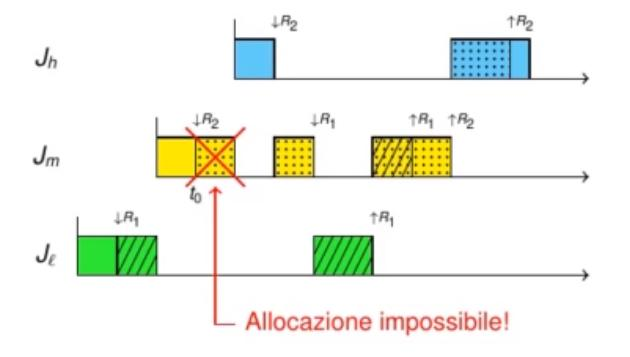
\includegraphics[scale=0.4]{immagini/image-027.jpg}
\end{figure}
J$_{l}$ sta bloccando J$_{m}$ e J$_{m}$ sta bloccando J$_{h}$. Perché non può verificarsi:\\ $\pi_{h}$ $>$ $\pi_{m}$ $\pi_{l}$ $\Rightarrow$ $\lceil\rceil$(R$_{1}$) $\geq$ $\pi_{m}$ e $\lceil\rceil$(R$_{2}$) $\geq$ $\pi_{h}$.\\ Quindi $\lceil\rceil'$(t$\_{0}$) $\geq$ $\lceil\rceil$(R$\_{1}$) $\geq$ $\lceil\rceil'$t$_{0}$; quindi l'allocazione non può avvenire.\\
\subsubsection{Tempo di blocco per conflitto di risorse}
È il massimo tempo di ritardo un job del task T$\_{i}$ causato da un conflitto di risorse.\\ Come faccio per calcolarlo: ho 3 tipi di blocco, quindi devo calcolarlo per tutti e 3  tipi, mi il teorema mi dice che il job può essere bloccato per al massimo una sezione critica, quindi considero il massimo.esempio:\\ J$_{1}$:[R$_{1}$;0.8], J$_{2}$, J$_{3}$:[R$_{2}$;0.2], J$_{4}$:[R$_{1}$;1].\\ 
\begin{figure}[!h]
\centering
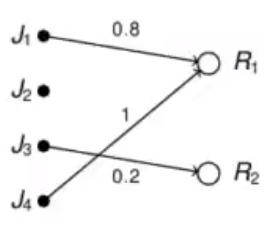
\includegraphics[scale=0.4]{immagini/image-028.jpg}
\end{figure}
J$_{4}$ può bloccare direttamente J$_{1}$ per 1 unità di tempo $\Rightarrow$ b$_{1}$(rc) = 1. J$_{4}$ può bloccare anche J$_{2}$ e J$_{3}$, quando acquisisce R$_{1}$ $\Rightarrow$ b$_{2}$(rc) = b$_{3}$(rc) = 1: può bloccare per priority inheritance. Sto facendo analisi pessimista: J$_{4}$ chiede la risorsa e subito dopo la chiede J$_{1}$. Il job per J$_{4}$ è b$_{4}$(rc) = 0, perché il job di priorità più bassa.\\ Per esempi più complessi, conviene avere un algoritmo automatico per derivare i tempi di blocco:
\begin{figure}[!h]
\centering
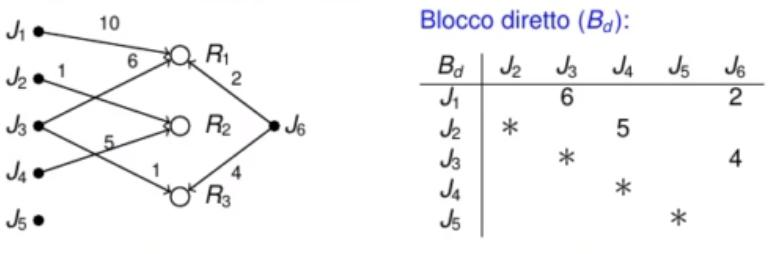
\includegraphics[scale=0.4]{immagini/image-029.jpg}
\end{figure}
\begin{itemize}
\item Costruisco una tabella dei tempi di blocco diretti. Su entrambe le colonne avrò i nomi dei job, ciascuna componente rappresenta il tempo di blocco diretto che il job della colonna fa subire al job della riga.\\ Le righe hanno i 5 job di priorità superiore mentre le colonne i 5 di priorità inferiore
\item Metto asterisco sugli elementi della "diagonale", ovvero le righe e colonne con lo stesso job, so che sotto la diagonale il blocco non può avvenire, quindi avrò valore 0.
\item Riempio le componenti sopra gli asterischi: vedo chi è in conflitto sulle varie risorse.
\end{itemize}
Posso derivare in maniera automatica la tabella per i blocchi dovuti all'inheritcance: 
\begin{figure}[!h]
\centering
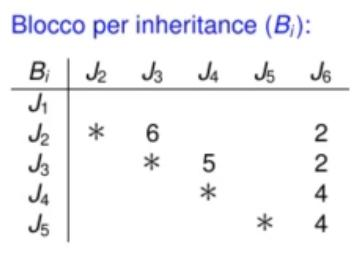
\includegraphics[scale=0.4]{immagini/image-030.jpg}
\end{figure}
\\avviene in caso di contesa, quindi quando un job nel blocca un altro viene trasferita la priorità. J$_{3}$ blocca J$_{1}$ per 6 unità di tempo. Ma allora il job di priorità intermedia può essere bloccato per 6 unità di tempo, quindi il 6 scende di una posizione nella tabella. Blocco tra J$_{2}$ e J$_{4}$, questo danneggia i job di priorità intermedia, ovvero J$_{3}$, il 5 scende fino alla riga di J$_{3}$.\\ J$_{6}$: blocca per inheritance anche tutti i job di priorità intermedia tra lui e J$_{1}$, e quindi tutti gli altri. Voci scendono sempre fino all'asterisco. Ad un certo punto, trovo che J$_{6}$ sta bloccando direttamente anche J$_{3}$, quindi per inheritance J$_{3}$ è bloccato per 2 unità di tempo, ma poi J$_{4}$ sarebbe bloccato per 2 unità di tempo a causa della contesa con J$_{1}$ ma anche per 4 unità per via della contesa con J$_{3}$. Devo considerare il worst case: ora è 4, quindi è il 4 a propagarsi verso il basso.\\ Infine ho la tabella per il blocco per priority ceiling:\\
\begin{figure}[!h]
\centering
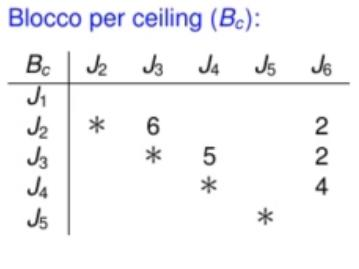
\includegraphics[scale=0.4]{immagini/image-031.jpg}
\end{figure}
Questo diventava simile al blocco per inheritance: J$_{4}$ può essre danneggiato da J$_{6}$ perché J$_{6}$ richiede risorsa che innalza il priority ceiling, caso peggiore è il max fra la lunghezza della regione critica fra R$_{1}$ ed R$_{2}$ (per J$_{6}$). Siccome J$_{5}$ non richiede risorse, manca il valore perché J$_{5}$ non può mai essere bloccato in quanto non richiede risorse.\\ A questo punto posso definire B$_{i}$(r,c) = max\{B$_{d}$(j, c): 1 $\leq$ j $\leq$ r-1\}.\\ Se le priorità dei job sono tutte diverse, B$_{c}$ = B$_{i}$, tranne che per i job che non utilizzano risorse.\\ b$_{i}$(rc) = max$_{k}${B$_{d}$ B$_{i}$(j, k), B$_{c}$(i, k)}: considero il valore massimo per ciascuna riga, perché priority ceiling mi dice che blocco al massimo 1 volta. Cosa cambiare se i job possono avere priorità identiche?
\subsection{Schedulabilità con priority ceiling}
Ho i tempi di blocco, li considero tra i tempi di blocco totali dei task, lo faccio task per task:\\
b$_{i}$ = b$_{i}$(ss) + (K$_{i}$ + 1)$\cdot$b$_{i}$(np) + (K$_{i}$ + 1)$\cdot$b$_{i}$(rc), con K$_{i}$ massimo numero di auto-sospensioni di un job del task T$_{i}$. Il fatto dell'unicità del job bloccante vale solo se i job non si auto-sospendono. Devo anche tenerne conto all'overhead su cambi di contesto: e$_{i}$' = e$_{i}$ + 2$\cdot$(K$_{i}$ + 1)$\cdot$CS + 2$\cdot$(K$_{i}$ + 1)$\cdot$CS, ma solo se il job usa le risorse condivise.
\subsection{Protocollo stack-based priority-ceiling}
Baker, 1991. È una semplificazione del protocollo priority-ceiling, motivato da un esigenza particolare: la condivisione di un unico stack da parte dei job. Usare uno stack unico comporta problemi: stack è LIFO, ogni volta che arriva un job sopra, interrompe quello sotto. Se un job arriva e richiede una risorsa, ma poi arriva una altro job che interrompe: comincia ad usare lo stack, in una zona contigua a quel job interrotto. Quando il job si conclude, toglie dallo stack tutte le informazioni che aveva introdotto. Ma se il jbo richiede la stessa risorsa del job che ha interrotto: per priority ceiling deve tornare in esecuzione il job interrotto. Probelma: il job non può togliere le info dallo stack ed ora il job che torna si trova una parte dello stack occupato.\\ Questo porta al fatto che nessun job deve bloccare o auto-sospendersi.\\ Per ogni risorsa R, $\lceil\rceil$(R) definito come nel protocollo priority-ceiling. C'è regola di aggiornamento che  è la stessa. \\ Regola di schedulazione: non appena rilasciato, un job J con priorità maggiore assegnata $\pi$ non può essere eseguito finché non è vera la condizione $\pi$ $\leq$ $\lceil\rceil$'(t). I job eseguibili sono schedulati in modo interrompibile in accordo alle priorità assegnate.Non c'è priority inheritance\\ Regola di allocazione: quando un job richiede una risorsa, la richiesta è soddisfatta.\\ Un job di priorità alta può interrompere un job di priorità bassa, e quest'ultimo non può tornare in esecuzione finché il primo non ha finito. Potrebbe farlo se il job bloccasse, ma questo non succede perché risorsa è libera o se si auto-sospendesse, ma qui questo non avviene. Quando un job comincia l'esecuzione tutte le risorse di cui ha bisogno sono libere: difatti inizia solo se la sua priorità diviene uguale o maggiore del priority ceiling del sistema.\\ Non ci sono mai deadlock: le risorse sono sempre libere quando le richiedo. Job non i auto-sospendono: il controllo d'accesso è effettuato solo al rilascio di un job e assume che il job non venga sospeso.\\ esempio di schedulazione:\\
\begin{figure}[!h]
\centering
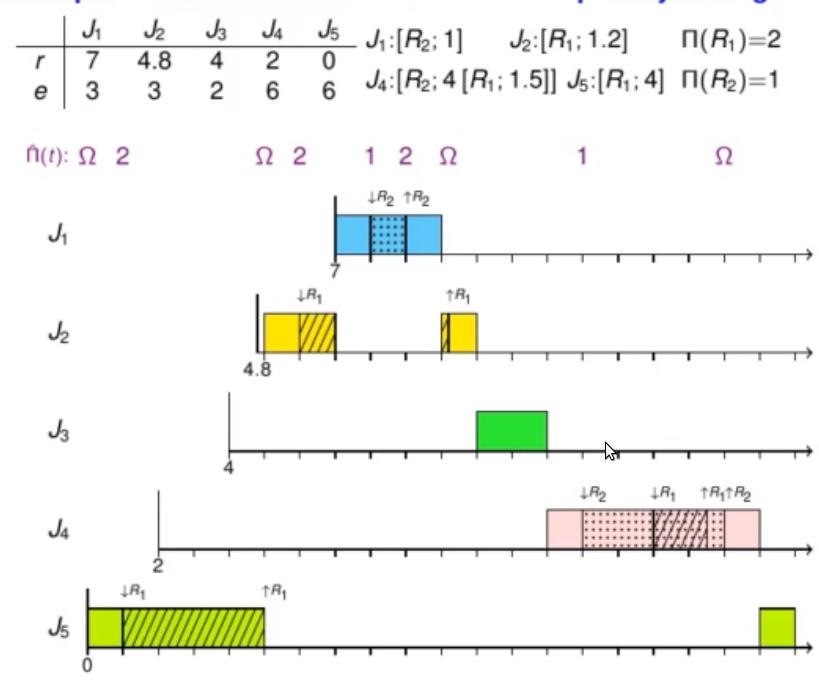
\includegraphics[scale=0.4]{immagini/image-032.jpg}
\end{figure}
\subsection{Ceiling priority}
Usato nel Real-time System Annex di Ada95: linguaggio molto usato negli USA. È stato definito dal governo per lo sviluppo del sw in tutte le commesse militari.\\ Regola di schedulazione:
\begin{itemize}
\item Se un job non possiede alcuna risorsa, la sua priorità è quella rassegata dallo scheduler
\item Se un job possiede una risorsa, la sua priorità è uguale al massimo priority ceiling di tutte le risorsa assegnate al job.
\end{itemize}
Job con priorità identica sono schedulati in modo FIFO.\\ Regola di allocazione: quando un job richiede una risorsa la ottiene. Risorsa è sempre libera: se fosse occupata, il job che la sta usando avrebbe priorità almeno uguale a quello che la sta richiedendo.\\ Differenza fra stack-based e ceiling priority? Senza auto-sospensione le schedulazioni prodotte sono identiche. Però in ceiling-priority è possibile modificare le regole per permettere auto-sospensione.\\ Confronto tra i protocolli: Teorema(Baker, 1911): I tempi di blocco massimi b$_{i}$(rc) dovuti ai conflitti di risorse per priority-ceiling e per stack-based priority-ceiling sono identici. Quindi scheduler che usano stack-based o ceiling-priority sono più semplici ed efficienti, in più hanno meno context-switch. Però i cambi di prioirtà dinamiche sono meno frequenti in priority-ceiling, che ci sono solo in caso di contesa.\\ Trade off, ma spesso vincono gli ullimi due
\subsection{Controllo d'accesso per job con auto-sospensione}
I vari protocolli vanno adattati all'auto-sospensione:
\begin{itemize}
\item NPCS: non è possibile auto-sospendersi in una sezione critica
\item Priority-inheritance: se un job J è bloccato su una risorsa posseduta da un job J' auto-sospeso, la priorità dinamica di J' è aggiornata solo se $\pi$(t) $>$ $\pi$(t')
\item Priority-ceiling: non funziona più unicità del blocco
\item Stack-based: non esiste
\item Ceiling-priority; se un job si auto-sospende in una sezione critica, nessun job di priorità inferiore o uguale può essere eseguito. È come se nullificasse i vantaggi dell'auto-sospensione nelle sezioni critiche
\end{itemize}
esempio: auto-sospensione\\
\begin{figure}[!h]
\centering
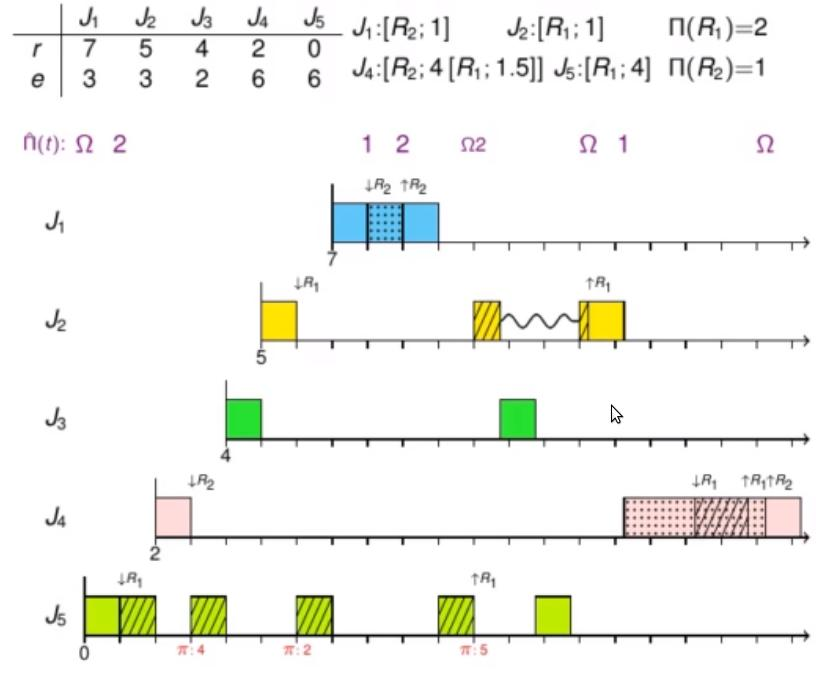
\includegraphics[scale=0.4]{immagini/image-033.jpg}
\end{figure}
Tempi di blocco per autosospensione
\begin{itemize}
\item NPCS: b$_{i}$ = b$_{i}$(ss) + (K$_{i}$ + 1)$\cdot$max\{b$_{i}$(np), b$_{i}$(rc)\}
\item priority ceiling e ceiling priority: b$_{i}$ = b$_{i}$(ss) + (K$_{i}$ + 1)$\cdot$ (b$_{i}$(np) + b$_{i}$(rc)). Qui i tempi di blocco b$_{i}$(rc) vanno calcolati anche pensando che mentre sono in sezione critica posso auto-sospendermi, quindi debo considerare anche il tempo massimo di auto sospensione e moltiplicare per il numero di volte in cui mi auto-sospendo.
\end{itemize}
\subsection{Priorità dinamica}
È possibile applicare i protocolli priority-ceiling e ceiling-priority a sistemi con priorità dinamica. Il valore del priority ceiling di una risorsa non è costante, ma dipende dalla priorità dinamica che potenzialmente fanno uso della risorsa. Il priority ceiling può cambiare, ad esempio con EDF ogni volta che rilascio un nuovo job, questo ha una prioirtà dovuta alla scadenza assoluta che fa cambiare i valori di priorità di tutti ti job del sistema, quindi i, pririty ceiling delle risorse e quindi il current priority ceiling del sistema. Molto poco applicabile nella realtà. Quando schedulo con algoritmi a priorità dinamica uso o NPCS o priority inheritance o altri sistemi per evitare deadlock come allocare risorse in tempi predefiniti.\\ esempio di priority ceiling con EDF:\\
\begin{figure}[!h]
\centering
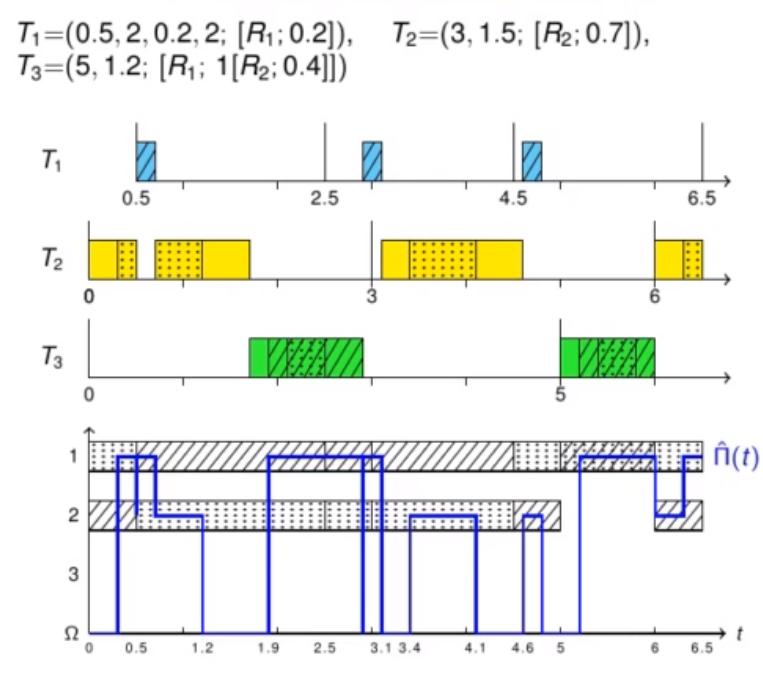
\includegraphics[scale=0.4]{immagini/image-034.jpg}
\end{figure}
\subsection{Accesso alle risorse di job aperiodici}
Problema: un server procrastinabile che sta eseguendo un job aperiodico esaurisce il budeget mentre il job è in sezione critica:
\begin{itemize}
\item Esecuzione all'interno della sezione critica rende il server non interrombilile anche se il budgrt finisce
\item Se ho accumulato ritardo, rifornisco meno budget.
\item Problema di schedulabilità e ritardi aggiuntivi, devo aggiungere anche la lunghezza della sezione critica dei job aperiodici. Questo comporta difficoltà nello studio, ma è modellabile
\end{itemize}
\chapter{Real-time su multiprocessore}
\section{Real-time su multiprocessore}
Ho rimosso man mano le limitazioni complicando il modello, rilasso l'ipotesi di avere un singolo processore(ultima limitazione rimasta).\\ Sistema multiprocessore ha 2 o più processori, ciascuno può eseguire job in maniera indipendente.\\ Processori possono essere dello stesso tipo o di tipo diverso:
\begin{itemize}
\item diversi microprocessori mutli-core
\item diverse schede di rete
\item diverse schede PCI con controllori DMA
\end{itemize}
In un certo senso, per cercare di modellare il sistema avrò $\mu$ tipi di processori quanti processori m$_{i}$ ci sono per i $\leq$ i $\leq$ $\mu$, anche su quali tipi di processore si può eseguire ciascun job. Semplifico supponendo che tutti i processori sono dello stesso tipo.\\ Ci si è resi conto molto presto che aggiungere processori complicava le cose: molto più complesso che schedulare su singolo processore.
\subsection{Sistemi statici}
Un sistema real-time è statico se ciascun job è assegnato perennemente ad uno specifico precessore. Partiziono i task nel sistema tale che ciascun job o task è eseguito forzatamente da uno specifico precessore: posso effettuare la schedulazione normalmente, ciascuno ha una lista di job e mi riconduco al caso del singolo processore (non proprio così).\\ 2 tipi di sistemi statici:
\begin{itemize}
\item L'assegnazione dei job è effettuata manualmente dal progettista una volta per tutte in fase di progettazione del sistema. Problema: devo conoscere tutti i parametri dei task, non posso gestire nuovi task che arrivano a run time
\item L'insieme dei task è assegnato ad uno specifico processore dal SO (o scheduler) durante la fase di creazione del task. Scheduler partizionati.
\end{itemize}
In entrambi i casi, lo scheduler non decide su quale processore sarà eseguito un job appena rilasciato.\\ esempio di schedulazione:\\
\begin{figure}[!h]
\centering
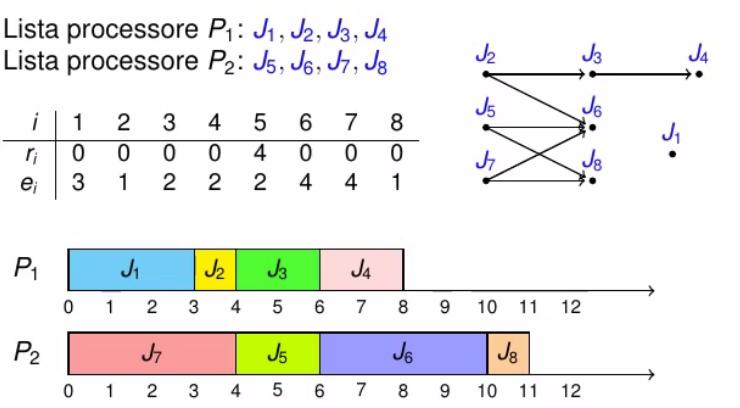
\includegraphics[scale=0.4]{immagini/image-035.jpg}
\end{figure}
\\I job hanno delle dipendenze: questo fa capire che il sistema non è analogo a tanti sistemi mono-processore, non ci sarebbero vincoli fra job su processori diversi. Ogni scheduler decide i job assegnati ai processori, ma i vincoli di dipendenza sono grosse complicazioni.\\ Vantaggi:
\begin{itemize}
\item Si può analizzare la schedulabilità su  ciascun processore usando i risultati teorici validi per il caso mono-processore
\item Se un job va in overrun (impiega più tempo del previsto) può ritardare l'esecuzione dei soli task che sono sul suo stesso processore (se job sono indipendenti tra di loro)
\item Se un job è interrotto, siccome il sistema è statico riprenderà l'esecuzione sullo steso processore, evito i costi dovuti alla migrazione
\item La coda di esecuzione è relativa al singolo processore ed è quindi più piccola
\end{itemize}
\subsection{Sistemi dinamici}
Un sistema real-time è dinamico se lo scheduler assegna dinamicamente un job ad un qualunque processore disponibile
3 varianti:
\begin{itemize}
\item Con job interrompibili
\item Con job interrompibili e non migrabili: anche se interrotto, job è salvato in una struttura locale del processore e potrà recuperare l'esecuzione solo si quel processore
\item COn job interrompibili e migrabili: job può essere migrato se interrotto, ha un costo
\end{itemize}
Una algoritmo di schedulazione per un sistema dinamico è globale perché stabilisce quale processore eseguirà quale job. \\esempio:\\
1° caso: job interrompibili e migrabili:\\
\begin{figure}[!h]
\centering
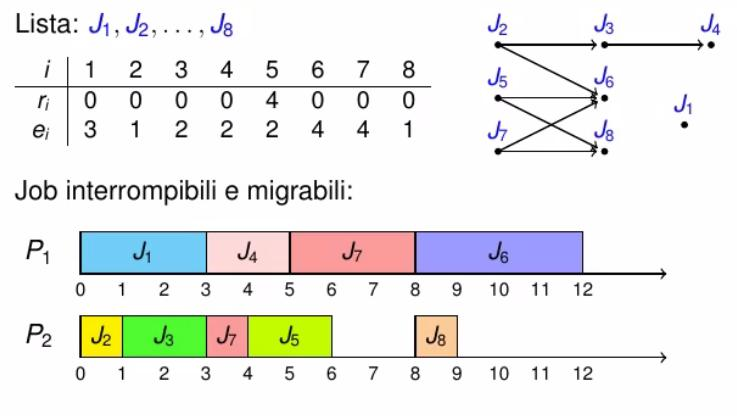
\includegraphics[scale=0.4]{immagini/image-036.jpg}
\end{figure}
2° caso, job non interrompibili:
\begin{figure}[!h]
\centering
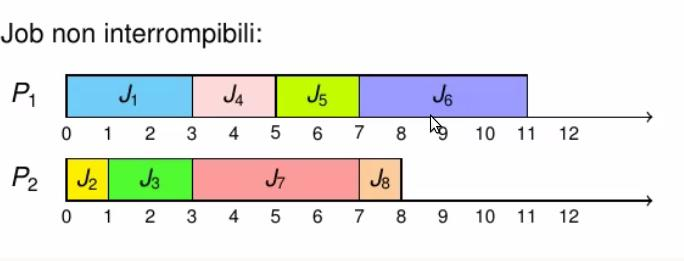
\includegraphics[scale=0.4]{immagini/image-037.jpg}
\end{figure}
\\Il momento in cui l'ultimo job completa il lavoro è uguale nel caso dei job migrabili a quello della schedulazione nel sistema statico $\Rightarrow$ anomalia di schedulazione.\\ Vantaggi:
\begin{itemize}
\item Hanno tipicamente meno cambi di contesto: quando viene rilasciato un job, in un sistema statico se c'è in esecuzione job di priorità minore devo interrompere e fare context swtich. In sistema dinamico posso avere processori free, quindi metto in esecuzione lì.
\item Se un job esegue per meno tempo di quello che è il suo worst case, il tempo liberato sul processore può essere utilizzato potenzialmente da tutti i task de sistema (nel caso del sistema statico è usato solo da quelli locali al processore).
\item Se un job impiega più tempo (overrun) la probabilità che questo comporti la mancanza di una op più scadenze è minore. Non è contrapposizione con 2: sistema può usare tutti i processori per cercare di porre rimedio al tempo in più per cui il job ha eseguito
\item Per ogni task del sistema che è creato a run-time, assegnazione e bilanciamento del carico sono "automatici" e determinati dall'algoritmo di schedulazione globale
\end{itemize}
\subsection{Algoritmi di schedulazione multiprocessore}
Gli algoritmi clock-driven sono in generale utilizzabili senza problemi, infatti la schedulazione avviene offline e validata una volta per tutte.Metodo però poco flessibile, ma non è immediato applicare algoritmi prioirty-driven, devo studiare bene come fare: devo risolvere diversi problemi
\begin{itemize}
\item Efficienza degli algoritmi, effetto Dhall
\item Predicibilità del sistema
\item Test di schedulabilità.
\end{itemize}
\subsection{Effetto Dhall}
Teorema (Dhall \& Liu): Per ogni numero di processori m $\geq$ 2, esistono insieme di task con utilizzazione bassa che non sono schedulabili con RM, DM o EDF.\\ Considero T$_{1}$=81, 2$\epsilon$), T$_{2}$=(1,2$\epsilon$,....,T$_{m}$=(1,2$\epsilon$), T$_{m+1}$?(1+$\epsilon$, 1). Utilizzazione globale = 2$\epsilon$ $\cdot$ m + $\frac{1}{1+ \epsilon}$ $\rightarrow$ 1 se $\epsilon$ $\rightarrow$ 0. Basterebbe uno o al massimo due processori per eseguire tutti questi task.\\ Ho una schedulazione fattibile: esempio per m=2\\
\begin{figure}[!h]
\centering
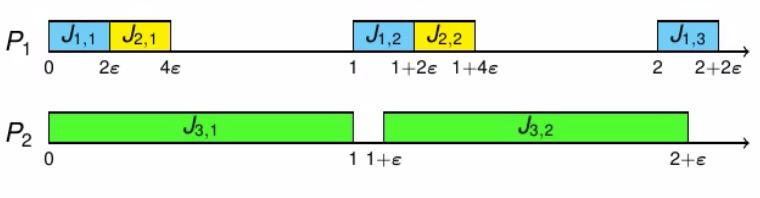
\includegraphics[scale=0.4]{immagini/image-038.jpg}
\end{figure}
Problema è che la schedulazione non è RM né DM né EDF: se schedulo con EDF vincono le scadenze assolute, quando tutti i job vengono rilasciati due job hanno priorità sugli altri, quindi quando i processori si liberano uno dei job manca la scadenza; stesso vale per RM e DM.\\ Questo risultato ha scoraggiato per tanti anni la ricerca su sistemi multiprocessore real-time, riprende quando siatemi multiprocessore si sono largamente diffusi da costringere a riguardare il problema: 2001, effetto Dhall esiste solo con sistemi di task in cui uno dei task ha un utilizzazione molto alta. Se task hanno utilizzazione non uguale ad 1 non si verifica l'effetto Dhall.
\subsection{Anomalie di schedulazione}
Comportamene di un algoritmo tale che, a fronte di variazione apparentemente vantaggiose dei parametri si hanno dei peggioramenti delle prestazioni. Esempi:
\begin{itemize}
\item Aumentano il periodo di un task
\item Aumento n° processori
\item Diminuisco il tempo di esecuzione di un task
\end{itemize}
Anomalie di schedulazione si verificano se task sono non interrompibili o indipendenti, nei sistemi uni-processore.\\ Nei sistemi multiprocessore? Mi metto nelle ipotesi che non ci siano vincoli di dipendenza:\\
\begin{itemize}
\item Sistema statico, job non interrompili: posso avere anomalie
\item Sistema statico, interrompibili: non ho anomalie
\item Sistema dinamico, job non interrompibili: posso avere anomalie
\item Sistema dinamico, job interrompibili ma non migrabili: sì
\item Sistema dinamico, job interrompili e migrabili: sì.
\end{itemize}
Perché le anomalie complicano la validazione? Non esiste un worst case a cui ricondursi, bisogna cercare un modo per tenere sotto controllo le anomalie.\\ esempio: anomalie di schedulazione con job non migrabili\\
\begin{figure}[!h]
\centering
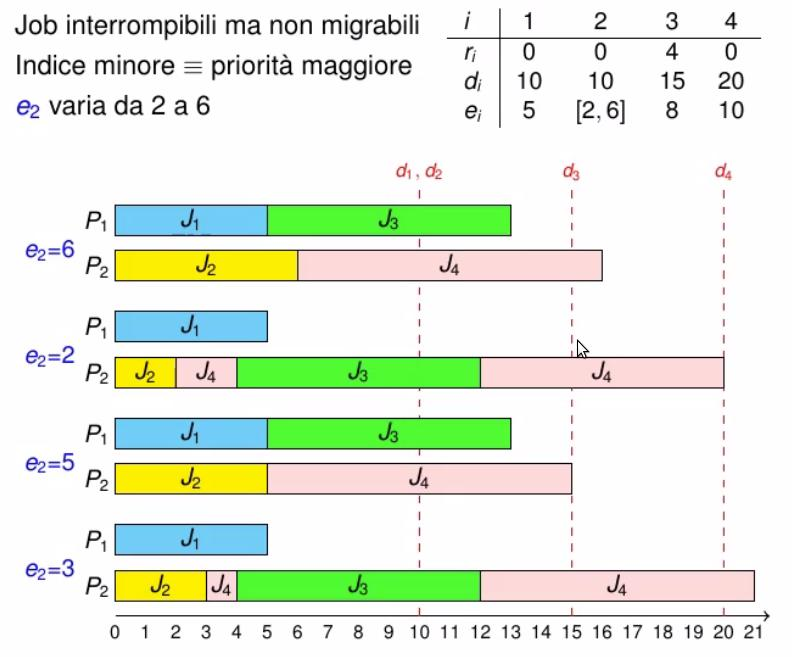
\includegraphics[scale=0.4]{immagini/image-039.jpg}
\end{figure}
anomalie di schedulazione con job migrabili:\\
\begin{figure}[!h]
\centering
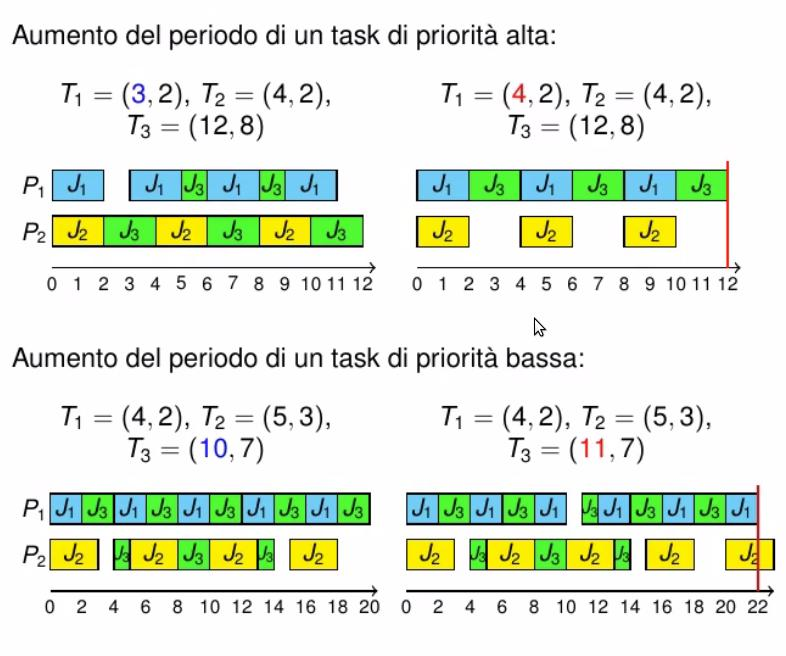
\includegraphics[scale=0.4]{immagini/image-040.jpg}
\end{figure}
\subsection{Schedulabilità}
Istanti critici in schedulazioni globali: c'è un teorema che mi dice che usando uno scheduler globale a priorità fissa a livello di task, l'istante in cui un job di un task T$_{i}$ è rilasciato contemporaneamente ai job di tutti i task di priorità superiore T$_{1}$,....,T$_{i-1}$ non è necessariamente un istante critico di T$_{i}$\\ esempio:\\
\begin{figure}[!h]
\centering
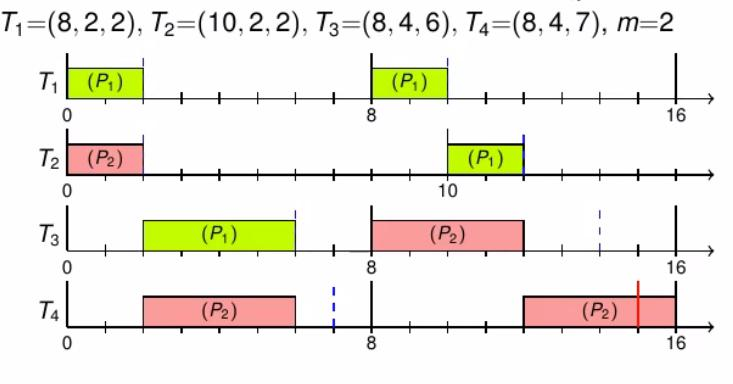
\includegraphics[scale=0.4]{immagini/image-041.jpg}
\end{figure}
\\Non ho modo di usare il test di schedulabilità.\\ Fattore di utilizzazione per multiprocessore: (thm) dato un sistema di task periodici con scadenze uguali ai periodi ed m processori, se X è un qualsiasi algoritmo di schedulazione partizionato con priorità fissa a livello di task:\\
U$_{X}$ $\leq$ $\frac{m + 1}{1 + 2^{\frac{1}{m +1}}}$. In pratica: se ad esempio uso RM, che ha su mono processore U$_{X}$ $\simeq$ 0.69, considerandolo partizionato il fattore di utilizzazione è limitato, non può in nessun modo utilizzarlo.\\ Teorema(2001): dato un sistema di task periodici con scadenze implicite ed m processori, sia X:
\begin{itemize}
\item un qualsiasi algoritmo di schedulazione partizionato
\item un qualsiasi algoritmo di schedulazione globale con priorità fissa a livello di job
\end{itemize}
allora per il fattore di utilizzazione di X si ha: U$_{X}$ $\leq$ $\frac{m + 1}{2}$.\\ Man mano che aumento il numero di processori, devo lasciarne sempre di più liberi. Sto quindi lavorando in perdita: se voglio aumentare di un processore il mio sistema, ne devo aggiungere 2 e cos' via...\\ Corollario: nessun algoritmo di schedulazione globale con priorità fissa a livello di job è ottimale su multiprocessore. Non posso sfruttare al 100\% tutti i processori del sistema.\\ esempio:\\
\begin{figure}[!h]
\centering
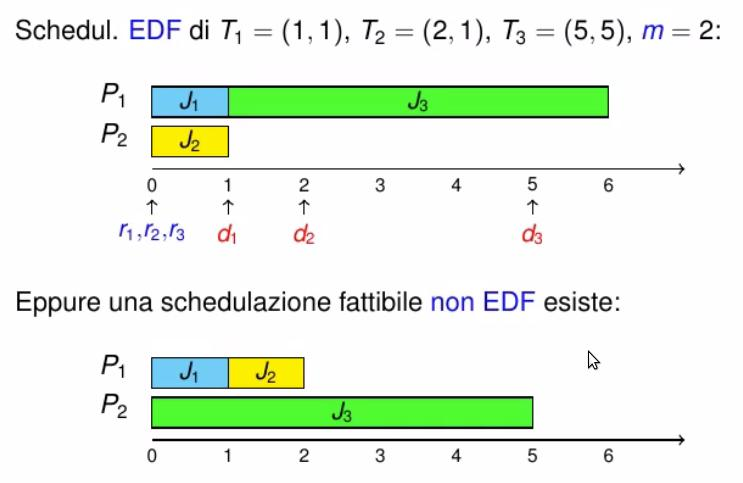
\includegraphics[scale=0.4]{immagini/image-042.jpg}
\end{figure}
\\Come si vede nell'esempio, schedulazione non EDF ottimale esiste.\\ Esistono algoritmi ottimali di schedulazione dinamica a livello di job che hanno fattore di utilizzazione pari ad m, esempio LST che però è complicato da implementare. Non esistono algoritmi on-line ottimali se gli istanti di rilascio dei job non sono esattamente prefissati.\\ Classe di algoritmi ottimali su multiprocessore è derivata dall'algoritmo Pfair:
\begin{itemize}
\item basati sul concetto di schedulazione fluida. Ogni task progredisce in modo proporzionale alla sua utilizzazione.
\item tempo diviso in quanti: allo scadere di ogni quanto, lo scheduler assegna i task ai processori in modo che per ogni task T$_{i}$, il lavoro compiuto sia $\lceil \frac{te_i}{p_i}\rceil$ o $\lfloor\frac{te_i}{p_i}\rfloor$.\\ Più è piccolo il quanto di tempo, più mi avvicino ad una schedulazione fluida, come in un SO in cui processi si alternano per quanti piccoli: sembra come se processi facessero progressi contemporaneamente
\end{itemize}
Gli algoritmi dinamici a livello di job sono molto costosi in termini di overhead dello scheduler. quindi non sono adottati.
\subsection{Schedulazione partizionata}
Nei sistemi real-time multiprocessore statici, l'algoritmo di schedulazione è partizionato. Non parlo di algoritmi in cui il progettista fissa i task ai processori, serve descrivere due componenti:
\begin{itemize}
\item Algoritmo che assegna i task ai processori (problema NP hard, non ammette algoritmo ottimale efficiente, tempi esponenziali nell'istanza del problema)
\item Algoritmo che schedula i task su ciascun processore
\end{itemize}
\subsubsection{Allocazione dei task}
Dato un sistema di task periodici,partizionare i task in sottoinsiemi tali che ciascun sottoinsieme può essere schedulato in modo fattibile su un singolo precessore utilizzando un determinato algoritmo do schedulazione.\\Un sistema di n task indipendenti è schedulabile con n processori (purché ciascun task abbia densità inferiore ad 1).\\ Non esiste algoritmo polinomiale che possa capire il più piccolo n° di processori per schedularlo. Gli algoritmi di schedulazione dei task possono solo calcolare soluzioni approssimate (non ottimali):
\begin{itemize}
\item Non riescono ad associare i task ai processori in modo da sfruttarli nel miglior modo possibile
\item Non riescono a determinare schedulabilità fattibili per ogni possibile insieme di task schedulabile
\end{itemize}
Limiti che non sono superabili.\\ Metriche di bontà:
\begin{itemize}
\item Rapporto di approssimazione: è il massimo valore $\frac{m}{m_0}$, dove m è il numero di processori usato dall'algoritmo di allocazione ed m$_{0}$ è  il minimo numero teoricamente necessario, considerando ogni possibile sistema di task. Buono se n° task è piccolo, m$_{0}$ non è facile da determinaste
\item Fattore di accelerazione: quanto è necessario aumentare la velocità di esecuzione degli m$_{0}$ processori per schedulare fattibilmente ogni possibile sistema di task le assegnazioni determinate dall'algoritmo di allocazione.
\item Fattore di utilizzazione: il valore di soglia per cui i sistemi di task con fattore di utilizzazione totale inferiore o uguale sono sempre schedulabilità utilizzando l'algoritmo di allocazione dei task.
\end{itemize}
\subsubsection{RMFF}
Il più semplice (Rate Monotonic First Fit), passi:
\begin{itemize}
\item ordina i task per periodi non decrescentisi T${1}$,...,T${n}$
\item ordina arbitrariamente i processori: P${1}$,...
\item comincia da T${1}$, assegna ciasun task T${i}$ al primo processore P${j}$ tale che l'insieme dei task già assegnati a P${j}$ insieme a T${i}$ risulta ancora schedulabile tramite RM.
\end{itemize}
U${RMFF}$ = m $\cdot$ ($\sqrt[2]{2}$ - 1).\\ Fattore di approssimazione: 2.23, usa un numero di processori che è 2.33 $\cdot$ numero ottimale (più del doppio). Non può essere usato come algoritmo on-line: siccome ordino per periodo non decrescenti, se arriva un nuovo task a run-time devo rifare tutto e quindi anche le assegnazioni, il che è impossibile. Usabile solo se conosco tutti i task in anticipo.
\subsubsection{FFDU}
Passi:
\begin{itemize}
\item ordina i task per periodi non decrescentisi T${1}$,...,T${n}$
\item ordina arbitrariamente i processori: P${1}$,...
\item cominciando da T$_{1}$, assegna ciascun task T$_{i}$ al primo processore P$_{j}$ tale che l'insieme dei task già assegnati a P$_{j}$ insieme a T$_{i}$ risulta ancora schedulabile tramite RM.
\end{itemize}
U$_{FFDU}$ = m $\cdot$ ($\sqrt[2]{2}$ - 1)\\ Fattore di approssimazione: 1.67. Poiché richiede di ordinare i task, comunque non è on-line.
\subsubsection{RM-FF}
Una variante di RMFF, che non effettua l'ordinamento dei task prima dell'allocazione:
\begin{itemize}
\item ordina arbitrariamente i processori: P${1}$,...
\item assegna ciascun task T$_{i}$ al primo processore P$_{j}$ tale che l'insieme dei task già assegnati a P$_{j}$ insieme a T$_{i}$ risulta ancora schedulabile secondo RM
\end{itemize}
U$_{RM-FF}$ = m $\cdot$ ($\sqrt[2]{2}$ - 1)\\ Fattore di approssimazione: 2.33.\\ A differenza di RMFF, RM-FF può essere usato on-line.
\subsubsection{EDF-FF}
Lo stesso algoritmo di RM-FF, ma schedulo il singolo processore con EDF:
\begin{itemize}
\item ordina arbitrariamente i processori: P${1}$,...
\item assegna ciascun task T$_{i}$ al primo processore P$_{j}$ tale che l'insieme dei task già assegnati a P$_{j}$ insieme a T$_{i}$ risulta ancora schedulabile secondo EDF
\end{itemize}
U$_{EDF-FF}$ = $\frac{\beta \cdot m + 1}{\beta + 1}$, $\beta$ = $\lfloor \frac{1}{\underset{k}{max}\frac{e_k}{p_k}}\rfloor$.\\ Fattore di approssimazione: 1.7 (meno del doppio del n° processori ottimali). È un algoritmo ottimale fra tutti gi algoritmi ottimali:\\ per $\beta$ = 1 $\Rightarrow$ U$_{EDF-FF}$ = $\frac{(m + 1}{2}$, ovvero nel caso peggiore ho il limite superiore nel caso in cui c'è un task di dimensione 1. Posso convivere con l'effetto Dhall, pagando processori in più. Se $\beta \rightarrow \infty$ $\Rightarrow$ U$_{EDF-FF}$ $\rightarrow$ m, per task di dimensioni infinitesima e quindi schedulabili in maniera fluida, l'algoritmo riesce a raggiungere il 100\% di utilizzazione dei processori del sistema.
\subsubsection{EDF-FFDD}
È possibile estendere gli algoritmi partizionati basati su "first fit" anche a task sporadici con scadenze arbitrarie.\\ EDF-FFDD:
\begin{itemize}
\item Ordina arbitrariamente P$_{1}$,P$_{2}$,...
\item Ordina i task sporadici per densità $\frac{e_i}{min(p_i, d_i)}$ decrescenti
\item Assegna ciascun task T$_{i}$ al primo processore P$_{j}$ tale che l'insieme dei task già assegnati a P$_{j}$ inseme a T$_{i}$ risulti ancora schedulabile secondo EDF
\end{itemize}
Condizione di schedulabilità:
\begin{itemize}
\item $\Delta_T$ $\leq$ m - (m-1)$\cdot$ $\Delta_{max}$ se $\Delta_{max}$ $\geq$ $\frac{1}{2}$
\item $\Delta_T$ $\leq$ $\frac{m}{2}$ + $\Delta_max$ se $\Delta_{max}$ $\leq$ $\frac{1}{2}$
\end{itemize}
\subsection{Scheduler multiprocessore globali}
Ha senso considerare scheduler globali non partizionati? Assumo tutti i job indipendenti, migrabili, interrompibili e senza auto-sospensione.\\ Ci sono anomalie di schedulazione, ma è utile rispetto ad EDF partizionato? Questo raggiunge l'ottimo, quindi mi chiedo se ne vale la pena, problema inoltre di istanti critici ed effetto Dhall.\\ Anomalie di schedulazione: il tempo di esecuzione dei task è worst case, teorema del 1994: sistemi di task periodici interrompibili e migrabili su multiprocessore schedulati con algoritmi a priorità fissa (a livello di task o job) sono predicibili, ovvero non presentano anomalie di schedulazione dipendenti dal tempo di esecuzione dei job.\\ Risolvo la più grave anomalia, ce ne sono altre.\\ Utilità rispetto ad EDF partizionato: so che EDF partizionato può ottenere l'ottimo, quindi perché considera algoritmi globali.\\ EDF ottimale tra gli scheduler partizionati basati su priorità fissa, ma non on senso assoluto: esistono algoritmi globali a priorità dinamica che raggiungono l'ottimo m, esempio Pfair.\\ Teorema: un sistema di task sporadici con scadenze arbitrarie è schedulabile con m processori con algoritmo globale a priorità dinamica a livello di job se: \\ $\Delta_T = \sum\limits_{i} \frac{e_i}{min_i{d_i, p_i}} \leq m$ e $\Delta_{max} = max_i \frac{e_i}{min{p_i, d_i}} \leq 1$.\\ Corollario: se le scadenze sono implicite, allora con un sistema di m processori ed un algoritmo globale a priorità dinamica a livello di job posso schedulare se:\\ $U_T = \sum\limits_{i} \frac{e_i}{p_i} \leq m$ e $U_{max} = max_{i} \frac{e_i}{p_i} \leq 1$.\\ Istanti critici: il rilascio in fase di tutti i job non corrisponde necessariamente ad un instante critico. Non posso usare la funzione di tempo necessario per analizzare se un sistema di task è schedulabile su un certo n° di processori. Uso  le condizioni di schedulabilità legate al fattore di utilizzazione o alla densità del task.\\ Effetto Dhall: è un problema che si verifica nei sistemi multiprocessore, per cui dato un qualunque n° di task che hanno utilizzazione totale costante rispetto ad m che non possono essere schedulati né con RM/DM né con EDF. L'effetto Dhall è condizionato dall'esistenza di un task che ha utilizzazione vicina all'unità, quindi posso cercare di correlare l'utilizzazione massima dei vari task con la schedulabilità del sistema.\\ Teorema: un sistema T di task sporadici con scadenze implicite,utilizzazione totale è U$_T$ e suppongo che valore dell'utilizzazione del task a priorità massima è U$_{max}$, allora il sistema è schedulabile con EDF globale su un sistema con m processori se: \\ U$_T$ $\leq$ m - (m-1) $\cdot$ U$_{max}$. Teorema va letto "all'opposto": se U$_{max}$ = $\frac{1}{2}$ allora ho come soglia di utilizzazione $\frac{m +1 }{2}$, ovvero il limite dei sistemi a priorità fissa a livello di job ,partizionati. Qui, se U$_{max}$ è $\leq$ $\frac{1}{2}$, la soglia tende ad m, quindi sistema può essere scheduabile anche se la soglia tende al numero totale di processori del sistema. Casi limite:
\begin{itemize}
\item U$_{max}$ = 1 $\rightarrow$ U$_T$ $\leq$ 1, Effetto Dhall
\item U$_{max}$ = 0 $\rightarrow$ U$_T$ $\leq$ m
\end{itemize}
Estensione del teorema per scadenze arbitrarie, teorema: Un sistema di task T, sporadici con scadenze arbitrarie, densità totale $\Delta_T$ e densità massima dei task $\Delta_{max}$ è schedulabile con EDF globale su un sistema con m processori se:\\ $\Delta_T$ $\leq$ m -(m-1)$\Delta_{max}$.\\ Esistono diverse altre condizioni di schedulabilità per EDF globale basate sulla densità dei singoli task e/o sul calcolo del tempo di processore richiesto dai task. È possibile avere algoritmi di schedulazione a priorità fissa (a livello di task o job) migliori di EDF globale per insiemi di task generici?\\ Considero EDF partizionato: ha una garanzia di schedulabilità che è $\frac{m+1}{2}$, certamente migliore della garanzia di schedulabilità di EDF globale, in quanto in quest'ultimo caso la garanzia è 1. Per insieme di task grandi, EDF partizionato va meglio, ma in generale gli algoritmi globali potrebbero andare bene o anche meglio di quelli partizionati per insiemi di task piccoli. Posso trovare algoritmi ibridi che vadano meglio di quelli visti fin ora?
\subsubsection{EDF-US[zeta]}
EDF-US[$\zeta$] è un algoritmo ibrido, proposto nel 2002, $\zeta$ è un parametro $\leq$ 1.\\ Una parte dei task ha priorità fissa, questi sono i task T$_t$ tali che $\frac{e_i}{p_i}$ $>$ $\zeta$, quindi sono tutti i task grandi.\\ Tutti hanno identica priorità, perché l'idea è che $\zeta$ è minore del numero di processori del sistema, quindi i task potranno sempre essere seguiti in parallelo.\\ Gli altri task hanno priorità più piccola dei task a priorità fissa e sono schedulati mediate EDF: la priorità non è più del task, ma del job. Hanno però priorità inferiore, quindi verranno sempre interrotti da quelli a priorità fissa. Idea: task grandi prendono sempre i processori disponibili,task piccoli prendono quello che rimane.\\ Non ho effetto Dhall: se ho task grandi, prendo processore, uso algoritmo globale per schedulare i task piccoli, quindi ebito l'effetto Dhall.\\ esempio:\\
\begin{figure}[!h]
\centering
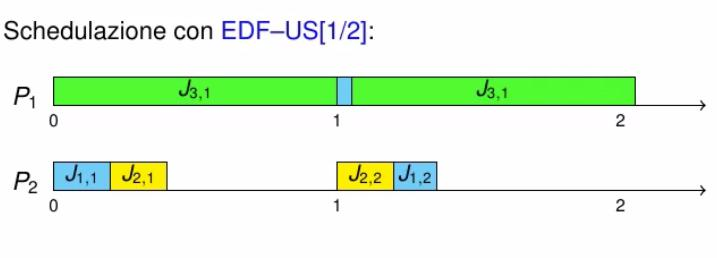
\includegraphics[scale=0.4]{immagini/image-043.jpg}
\end{figure}
Classico effetto Dhall se schedulo con EDF globale\\
\begin{figure}[!h]
\centering
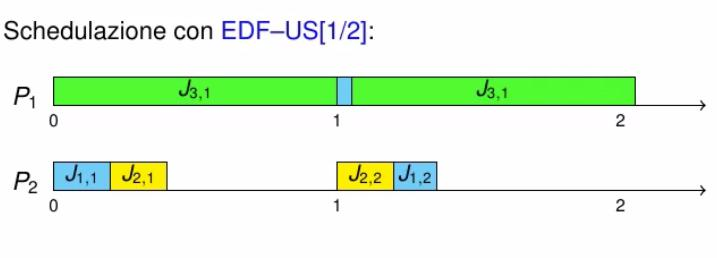
\includegraphics[scale=0.4]{immagini/image-044.jpg}
\end{figure}
\\Task T$_3$ ha utilizzazione $>$ $\frac{1}{2}$ ,quindi ha priorità fissa ed averà precedenza.\\ Prestazioni:\\ teorema: Un sistema di task sporadici implicite è  schedulabile secondo EDF-US[$\frac{m}{(2m-2)}$] su m processori è U$_T$ $\leq$ $\frac{m^2}{(2m-2)}$.\\ Corollario: Un sistema di task sporadici con scadenze implicite è schedulabile con EDF-US[$\frac{1}{2}$] su m processori se $U_T$ $\leq$ $\frac{m + 1}{2}$. Ottengo il meglio, continuano a valere le ipotesi del teorema visto in precedenza (Andersson).\\ Posso esistere algoritmi di schedulazione globale a priorità fissa migliori di EDF-US[$\frac{1}{2}$]: non devo confondere la garanzia di schedulazione data da questa condizione con l'effettiva capacità di shedulare sistemi di task generici
\subsubsection{EDF(k)}
Algoritmo ibrido, variante del precedente: k è un parametro, $<$ m. Una parte dei task ha priorità fissa, i primi k-1 con fattore di utilizzazione $\frac{e_i}{p_i}$ $>$ più alti; tutti gli altri hanno priorità dinamiche e sono schedulati con EDF.\\ L'idea è sempre la stessa: assegno i task grandi ai processori disponibili, gli altri li schedulo con EDF. Garanzie di schedulabilità:\\ Teorema: Un sistema di task sporadici con scadenze implicite è schedulabile con EDF(k) su m processori se: (k-1) + $\rceil \frac{U_t - u_k}{1 - u_k}\lceil$ $\leq$ m; dove u$_{k}$ è  il fattore di utilizzazione del k-esimo task.\\ Algoritmo EDF(k$_{min}$): Sia fissato m (in numero di processori), e sia k$_{min}$ il minimo valore di k che soddisfa la condizione del teorema precedente. Un sistema di task sporadici con scadenze implicite è schedulabile con EDF(k$_{min}$) se U$_T$ $\leq$ $\frac{m+1}{2}$.\\ Vale quanto detto prima: l'insieme dei task schedulabili con EDF-US[$\frac{1}{2}$] è un sotto-insieme proprio di EDF(k$_{min}$). Se guardo insieme di task con utilizzazione maggiore di $\frac{m+1}{2}$ EDF(k$_{min}$) schedula più job rispetto ad EDF-US[$\frac{1}{2}$], non confondere con la garanzia di schedulabilità.
\subsubsection{Scheduler globali basati su priorità fissa a livello di task}
Questo tipo di algoritmi non può essere migliore di algoritmi globali o ibridi a priorità dinamica a livello di task, questo perché l'algoritmo sottostante che uso su un sistema mono-processore non può andare meglio. Ho visto che algoritmi partizionati vanno meglio in generale su insiemi di task generici (per via dell'effetto Dhall) di algoritmi globali. Il discorso della partizione in insiemi di task viene recuperati dagli algoritmi ibridi: ho un certo criterio per assegnare la priorità massima, i restanti task continuo a schedularli con un criterio differente, la priorità è legata all'algoritmo sottostante. Priorità è fissa perché è dovuta ad un condizione specifica, algoritmi globali a priorità fissa soffrono comunque dell'effetto Dhall, non possono andare meglio di algoritmi partizionati, e lo stesso vale per algoritmi ibridi: faccio assegnazione dei task a priorità massima che non dipende dall'algoritmo sottostante, quando schedulo i restanti job, schedulare con priorità fissa non può dare vantaggio rispetto a schedulare co priorità dinamica.\\ Questi algoritmi posso essere adottati:
\begin{itemize}
\item Semplici da implementare
\item Presenti su tutti i SO real-time
\item Sono più robusti in caso di job che superano il WCET calcolato in fase di design.
\end{itemize}
\subsubsection{Scheduler RM globale}
Teorema: un sistema di task periodici con scadenze implicite tale che U$_{max}$ $\leq$ $\frac{m}{(3m - 2)}$ è schedulabile con RM su m processori se: U$_{T}$ $\leq$ $\frac{m^2}{(3m - 1)}$. Tiene conto dell'effetto Dhall, limita l'utilizzazione del task più ingombrante a $\frac{m}{(3m - 2)}$, se la condizione vale l'effetto Dhall è evitato e posso aumentare il carico del sistema pur di aumentare il n° di pressori, sto andando sempre in perdita.\\ Teorema: un sistema di task sporadici con scadenze implicite è schedulabile globalmente con RM su m processori se U$_T$ $\leq$ $\frac{m}{2} \cdot (1 - U_{max}) + U_{max}$. \\ Posso anche riformulare i teoremi in termini di densità, ma le cose si complicano parecchio.
\subsubsection{RM-US[zeta]}
RM-US[$\zeta$] è un algoritmo ibrido analogo a EDF-US[$\zeta$], la differenza è che tutti i task che hanno utilizzazione inferiore alla soglia $\zeta$ sono schedulati con RM. Stessa idea: do priorità massima ai task ingombranti. Prestazioni:\\
teorema: Un sistena di task peridoti con scadenze implicite è schedulabile con RM-US[$\frac{m}{(2m - 2)}$] su m processori se: U$_T$ $\leq$ $\frac{m^2}{(3m - 2)}$\\ Teorema (2003): Un sistema di task sporadici con scadenze implicite è schedulabile secondo RM-US[$\frac{1}{3}$] su m processori se: U$_T$ $\leq$ $\frac{(m+1)}{3}$. Passare da EDF a RM fa si che $\frac{2}{3}$ dei processori rimangono inutilizzati.\\Il miglior valore di soglia è $\zeta$ = 0.37482, con utilizzazione massima pari a 0.37482$\cdot$(m+1), più restrittivo del 0.3333... del risultato precedente, ma così ho utilizzazione ottima.
\subsection{Possibile applicabilità degli algoritmi in sistemi real-time}
Algoritmi sono applicabili, ma problema grande nei sistemi multiprocessore è che gli algoritmi sono basati su ipotesi fondamentali:\\
indipendenza dei task fra di loro: inserire il discorso dei vincoli di dipendenza complica molto il discorso, non ho grandi risultati già stabiliti e consolidati.Problema è ancora più serio: i vincoli di dipendenza fra task potrebbero essere nascosti. Esempio: sistema reale multiprocessore, diversi core e diversi processori, quindi sistema parallelo con multiprocessore a loro volta mutlicore. Dal punto di vista hw, i core condividono risorse hardware: posso avere unità ALU individuale, am non è detto che non usino una singola MMU, singola cache L2/L3, processori diversi possono avere dipendenze legate ai tempi di accesso alla RAM o al bus di sistema. WCET: tempo massimo fi esecuzione quando job esegue da solo, ma se lo eseguo su sistema multiprocessore, questo verrà comunque rallentato dagli altri job su altri core perché magari c'erano ipotesi di indipendenza sbagliate. Le assunzioni di base sul worst case è falso, se presento sistema multicore a ente certificatore, non verrà mai accettato, perché è falsa assunzione di fondo del fatto che job su processori diversi non abbiano differenze. Punto cruciale della ricerca: realizzazione di sistemi single core equivalent: sistemi che operano sui singoli core come se fossero da soli, ma in realtà sono in un sistema multi-core.\\ Per avere certificazione: nel sistema di task bisogna prevedere task a priorità massima che entri in esecuzione periodicamente e spenga tutti i processori nel sistema tranne 1, non voglio che più di un processore sia attivo, altrimenti no bollino certificazione real-time.\\ Ricerca in divenire, c'è ancora problema di applicabilità in pratica dei risultati.
\chapter{Sistemi operativi real-time}
\section{Sistemi operativi real-time}
Obiettivi di un sistema operativo:
\begin{itemize}
\item Fa funzionare i driver, interazione con l'hardware, usando apposite procedure detti driver
\item Controllo dell'uso delle risorse hardware (massimizzazione durata batteria, salva schermo)
\item Costruzione di un'astrazione dell'architettura fisica, ambiente di esecuzione delle applicazioni
\item Offrire interfacce di accesso ai dispositivi hardware, utilizzo in maniera controllata
\item Distribuisce le risorse tra le varie applicazioni/utenti
\item Implementa servizi di comunicazione tra applicazioni locali o remote
\item Nei SO multitasking (tutti praticamente ormai) è possibile eseguire contemporaneamente più processi, shcduler assegna CPU di volta 
in volta.
\item Consente accesso a più utenti in contemporanea
\end{itemize}
Questi sono SO general purpose. In cosa differiscono da un SO real-time? Di fatto, la reale differenza sta nel tipo di applicazioni che i due SO devono eseguire: un applicazione real-time ha dei vincoli temporali da rispettare, ed anche il SO va progettato intorno all'idea che le applicazioni devono poter rispettare questi vincoli. SO real-time devono fare in modo che l'applicazione sia affidabile e predicibile.\\ Talvolta, le applicazioni real-time devono avere dei tempi di risposta rapidi, ma non è una proprietà caratterizzante. Questo non è però il punto cruciale dei SO real-time o delle applicazioni real-time, sono caratterizzate dal fatto che le scadenze vengono rispettate,qualunque esse siano.\\ So che la maggior parte dei sistemi real-time sono embedded, quindi sistemi operativi rea-time devono essere anche embedded, applicazioni devono quindi essere:
\begin{itemize}
\item Compatte
\item Scalabili
\item Consumo ridotto delle risorse, viste le esigenze dei sistemi embedded
\end{itemize}
\subsection{RTOS a microkernel}
Molti SO per sistemi embedded e RT sono basati su un modello a micro-kernel. SO real-time è un supporto generico ad applicazioni real-time, deve far si che funzioni correttamente e tutti gli altri compiti del SO, ma l'obbiettivo prioritario è il rispetto delle scadenze, quindi spesso molte delle feature del SO general purpose vengono sacrificate.\\ Micro-kernel è un piccolo programma che realizza pochi servizi essenziali, parte del codice del SO che esegue a livello di privilegio più alto possibile. Non tutte le parti del SO eseguono alla priorità massima, alcune potrebbero eseguire a livello di privilegio più basso. Feature del micro-kernel:
\begin{itemize}
\item driver dei circuiti, HW di base (tipicamente solo delle periferiche fondamentali)
\item schedulazione dei processi
\item comunicazione bi base fra i processi
\end{itemize}
Tutti gli altri servizi sono fatti al di fuori del kernel (driver delle periferiche, stack di rete. file system etc...)
Approccio differente al kernel monolitico: a livello user mode girano librerie di sistema per supporto ad applicazioni, tutto il resto viene eseguito in kernel mode.\\ Vantaggi del micro-kernel ai SO real-time: è approccio elegante, ma di base inefficiente perché applicazione moderna deve fare molte cose: interazione con FS, interazione con la rete etc..., bisogna scambiare informazioni e molti dati fra processi, nell'approccio micro-kernel le applicazioni per fare una semplice cosa devono coinvolgere decine e decine di processi utente separati.\\ Qui la velocità non è più primaria: mentre quando progetto SO general purpose voglio utilizzo efficiente da parte del SO delle risorse, mentre nel SO real-time no, voglio rispettare le scadenze. Il micro-kernel ha poco codice, quindi è più semplice verificarne la correttezza,ma poi devo anche verificare codice es dell'applicazione di rete: ma un conto è verificare il codice alla massima priorità, un conto è partire da kernel corretto e verificare codice a livello utente: uniche ripercussioni sono relative all "gabbia" costruite intorno al processo.\\ Struttura del kernel monolitico: tipici esempi sono tutti i sistemi derivati da Unix, quindi Linux, FreeBSD, SunOS, Solaris.\\ SO a micro-kernel: QNX, GNU Hurd (Mach \& Four, BeOS,...\\ Sistemi ibridi: partiti come micro-kernel, ma dopo avere valutato le prestazioni e aver visto che erano pessime, hanno portato componenti da user mode a kernel mode. Approccio ibrido, esempi: Windows NT, Mac OS X,...
\subsection{Caratteristiche chiave di un RTOS}
Un sistema operativo che opera in contesto real-time ed embedded deve offrire:
\begin{itemize}
\item Predicibilità: risposte agli eventi esterni predicibile, cura nella gestione degli interrupt hardware.
\item Risposte efficienti ad eventi esterni, bassa latenza nei tempi di risposta (non nei tempi di risposta dei task dei job).
\item Gestione affidabile e precisa di eventi temporali:
\begin{itemize}
\item gestione dei timer e clock hardware con le relative interruzioni
\item gestione del tempo di sistema 
\item gestione di allarmi
\end{itemize}
\item Deve poter avere un modo per schedulare i task, deve essere a basso overhead e predicibile:
\begin{itemize}
\item implementazione di algoritmi deterministici
\item supporto al partizionamento dei task in sistemi multiprocessore: problemi teorici legati ai sistemi globali sono ancora in analisi.
\end{itemize}
\item Gestione della comunicazione e sincronizzazione dei task:
\begin{itemize}
\item memoria condivisa, code, segnali
\item primitive di sincronizzazione come semafori, lock.
\end{itemize}
\item Gestione della memoria
\begin{itemize}
\item memoria virtuale: ogni task nel sistema, quando usa indirizzo di memoria fa riferimento ad una cella differente da quella che usa un altro task con lo stesso indirizzo, non è detto sia necessario per sistemi con poca memoria/embedded
\item protezione dello spazio di indirizzamento, discorso diverso dalla memoria virtuale. L'accesso alla memoria da parte di un task verso le celle di un altro task è proibito, possibile realizzare protezione di memoria senza che ci sia memoria virtuale. Più importante in un sistema real-time rispetto ad avere memoria virtuale
\end{itemize}
\end{itemize}
Spesso le applicazioni embedded per sistemi real-time sacrificano la memoria virtuale e spazi di indirizzi separati: il software deve passare per analisi talmente tanto strette che l'accesso a memoria che non compete sarà semplice da verificare. Problemi più importanti: se verifico che non ci sono indipendenze tra i task ,automaticamente nessuno fa ciò che non deve e quindi altre feature divengono overhead.
\subsection{Interruzioni hardware}
Ogni occorrenza di una interruzione hardware deve essere gestita con procedura apposita livello kernel o user mode. Deve essere rapido il modo in cui il SO riconosce l'interrupt ed agisce per gestirlo: quando dispositivo hw genera interrupt, blocca la sua attività, quindi finché CPU non riconosce l'interruzione l'hw è congelato, poi la gestione dell'interrupt può essere fatta in tempi più lunghi.\\ Il tempo richiesto per la completa gestione dell'interrupt dipende dalla periferica hardware:
\begin{itemize}
\item La lettura dei dati da un sensore è breve
\item Traferire di grandi blocchi di dati, ad esempio dalla scheda di rete alla memoria o dalla memoria secondaria alla RAM.
\end{itemize}
In ogni caso, le interruzioni devono essere riconosciute nel minor tempo possibile, altrimenti le periferiche HW potrebbero mal funzionare. 1 linea di interruzione fisica di interruzioni in ogni dispositivo, una sola linea verso il processore, l'interruzione arriva al PIC ed il PIC asserisce la linea verso la CPU e dopo la conferma della CPU il PIC conferma la ricezione al dispositivo, il driver del dispositivo gestirà con apposita routine la situazione.\\ Gestione delle interruzioni hardware in più fasi:
\begin{itemize}
\item Interrupt handler: 
\begin{itemize}
\item Priorità elevata
\item da conferma della ricezione dell'interruzione al PIC
\item salva e recupera il contesto di esecuzione del processore
\end{itemize}
\item Interrupt service routine (IRS), specifica del dispositivo:
\begin{itemize}
\item priorità più bassa (ma generalmente superiore ai processi di sistema)
\item esegue operazioni specifiche per l'interruzione ed il dispositivo che l'ha generata.
\end{itemize}
\end{itemize}
\subsection{Schedulazione}
Uno dei punti fondamentali, devo assicurare che le applicazioni real-time rispettino le scadenze. Bisogna usare politiche di schedualzione facili, predicibili, tipicamente EDF.\\ SO real-time non supportano nessun tipo di analisi di schedulabilità o test di accettazione on-line per nuovi task. È il progettista che deve prevedere tutti i possibili carichi del sistema e vedere se qualcuno di questi missa le scadenze.Analisi è fatta dal progettista ed avallata dai test del sistema.\\ Schedulazione tipicamente prehemptive, quindi job interrompibili, perché altrimenti cominciano ad avere anomalie di schedulazione. Possibile specificare che alcuni job non siano interrompibili, di solito non job collaborativi, ovvero rilasciano periodicamente il processore per far si che venga utilizzato da altri job; il codice va analizzato dal progettista. Scheduler quasi sempre clock-driven, va considerato nell'analisi di schedulabilità. Generalmente, ogni SO offre livelli di priorità finiti: se ho più task del numero dei livelli di priorità? Perdita di schedulabilità: devo dire che due task hanno la stessa priorità e questo può comportare problemi.\\ Perdita di schedulabilità:\\ ho modellato un sistema e stabilito che mi servono $\Omega_n$ livelli di priorità, ma nel sistema ne posso avere solo $\Omega_s$ $<$ $\Omega_n$. Devo fare mapping fra le priorità assegnate a quelle di sistema $\pi_1$,...,$\pi_s$ dove: $\pi_i$ $\in$ \{1,2,...$\Omega_n$\} $\forall$ i. I $\pi_i$ sono ordinati in maniera crescente ed indicano come mappo le priorità reali: tutte le priorità assegnate numericamente, minori o uguali a $\pi_i$ sono mappate su $\pi_i$. In generale, tutte le priorità assegnate tra $\pi_{k-1}$+1 e $\pi_k$ sono mappate su $\pi_k$ $\forall$ 1 $<$ k $\leq$ $\Omega_s$.\\ Devo tenere conto di questo mapping nell'analisi di schedulazione, devo farlo task per task:\\ considero task T$_i$, siano T$_E$(i) e T$_H$(i) gli insiemi dei task di priorità uguale (il primo) e superiore a T$_i$, rispettivamente:\\ w$_i$ = e$_i$ + b$_i$ + $\sum\limits_{T_k \in T_E(i)} e_k$ + $\sum\limits_{T_k \in T_H(i)} \lceil \frac{t}{p_k} \rceil e_k$. Aggiungo nel caso peggiore che i task di priorità uguale portano via tempo, resta il fatto che lo scheduler schedula i task in modalità FIFO: se due task hanno pari priorità, uno può essere rallentato dal fatto che arriva dopo ad un altro di pari priorità, ma quando quello ha finito tocca a lui.\\
w$_{i,j}$(t) = j $\cdot$ e$_i$ + b$_i$ + $\sum\limits_{T_k \in T_E(i)} (\lceil \frac{(j-1)p_i}{p_k} \rceil + 1)e_k$ + $\sum\limits_{T_k \in T_H(i)} \lceil \frac{t}{p_k} \rceil e_k$. Applico lo stesso alla funzione di tempo necessaria per tempi arbitrari, stavolta considero dal rilascio del job che sto guardando in poi. Devo calcolare quanti job con la mia stessa priorità vengono rilasciati nell'intervallo che sto considerando (+1 è rilascio iniziale).\\ Associazione a rapporto costante: lo scheduler potrebbe non distinguere i job di priorità più alta. Si utilizza quindi in genere un'assegnazione  che riserva i livelli di priorità di sistema ai livelli di priorità assegnata più alti e mano a mano accorpa le priorità assegnate di livello più basso.\\ In pratica, si può cercare di mantenere approssimativamente costanti i rapporti: g$_k$ = $\frac{\pi_{k-1} + 1}{\pi_k}$ (1 $<$ k $\leq$ $\Omega_s$), maniera di assegnare le priorità migliore.\\ Teorema: Per l'algoritmo di scheduling RM,  con scadenze relative pari al periodo e numero n di task elevato, usando l'associazione a rapporto costante g = min$_{1 < k < \Omega_s} g_k$,allora U$_{RM}$:
\begin{itemize}
\item ln(2g) + 1 - g se g $>$ $\frac{1}{2}$
\item g se g $\leq$ $\frac{1}{2}$
\end{itemize}
La schedulabilità relativa indica la perdita di schedulabilità dovuta ad un numero limitato di livelli di priorità nel sistema: $\frac{U_{RM}(g)}{ln(2}$. Casi limite:\\ per g = 1 $\frac{U_{RM}(g)}{ln(2}$ = 1, quindi nessuna perdita\\ g = $\frac{1}{2}$ $\frac{U_{RM}(g)}{ln(2}$ = $\frac{1}{2ln2}$, quindi perdita del 28\%. Non dare per scontato che adattare il modello al caso reale non possa provocare problemi. Tutti i SO real-time consentono di usare algoritmi a priorità fissa, offrono delle API che consentono di impostare le priorità di task sulla base di deadline relativa. Pochi permettono di usare schedulazione dinamica a livello di task,come EDF: il reinserimento automatico dei task in coda a priorità nella posizione corretta in base alla deadline assoluta è inefficiente: servono strutture dati apposite o gestione di pochi task. È pericoloso gestire strutture dati complesse,quindi per avere efficienza bisogna ridurre numero di task supportati.
\subsection{Standard per RTOS}
Standard importanti:
\begin{itemize}
\item Portabilità dell'applicazione
\item Interoperabilità dei sistemi
\item Possibile cambiare real-time OS
\end{itemize}
Diversi standard:
\begin{itemize}
\item POSIX, estensione real-time
\item OSEK/CDX
\item ARINC/APEX
\item ITRON
\end{itemize}
\subsubsection{POSIX}
Estensione che definisce API per avere ad esempio:
\begin{itemize}
\item mutua esclusione con priority inheritance.
\item attesa e sincronizzazione tramite varabili condizione
\item memoria condivisa
\item code di messaggi a priorità
\item schedulazione preempitve con priorità fissa
\item server sporadici
\item gestione del tempo con alta risoluzione
\item possibile misurare e limitare il tempo di esecuzione dei task.
\end{itemize}
4 profili differenti dello standard:
\begin{itemize}
\item Minimal Real-Time System, per piccoli sistemi embedded: solo thread,n non processi e I/O tramite device file nessun file system.
\item Real-time COntroller, per sistemi robotici: come il precedente, ed in più un file system con ci gestire i file regolari
\item Dedicated Real-time System: per sistemi avionici, grandi sistemi embedded, multi-processo con meccanismi di protezione degli accessi alle risorse
\item Multi-purpose Real-time System: per sistemi general purprose con applicazioni sia real-time che non, tutti i servizi POSIX per i sistemi operativi general purpose
\end{itemize}
\subsubsection{OSEK/VDX}
Progetto congiunto di diverse industrie automobilistiche (BMW, Bosh, Opel) e l'università di Karlsruche. Definisce insieme di API per un sistema real-time integrato in un sistema di gestione di rete. Orientato a sistemi di controllo con vincoli real-time hard, alata criticità, grandi volumi di produzione. Tiene in grande considerazione l'ottimizzazione del codice, riduzione dell'occupazione di memoria e miglioramento delle prestazioni del RTOS.\\ Propone interfacce e protocolli ad alto livello per le comunicazioni interne del veicolo ed interfacce e protocolli per l'interoperabilità dei vari sistemi embedded all'interno dell'autoveicolo:
\begin{itemize}
\item politiche di accesso
\item meccanismi per la resistenza ai guasti
\item procedure di diagnostica della rete e di comunicazione
\end{itemize}
Un tipico sistema OSEK è scalabile, può usare diversi tipi di precessori, non prevede protezione di memoria. Deve produrre software portabile: tra l'applicazione ed il SO c'è uno strato di interfaccia scritto in ISO/ANSI-C. In ogni caso non vengono specificate interfacce verso i sistemi I/O.\\ IL progettista può usare degli strumenti di configurazione standard per definire i servizi e l'uso, viene proposto linguaggio OIL (Osek Impelmentation Language). L'allocazione è statica, ovvero tutte le strutture dati del kernel e dell'applicazione sono allocate staticamente.\\ Il supporto per architetture "time triggered" fornisce la specifica di un sistema operativo basato sul tempo.\\ Supporta architetture "time triggered", fornisce una specifica di un sistema operativo basato sul tempo che può essere completamente integrato nel framework OSEK/VDX. Ci sono le specifiche di un sistema real-time in questo stanard per sistema embedded
\subsubsection{ARINC 653}
Standard per sistemi avionici, progettazione e certificazione di sistemi safty-critical e real-time. Lo standard consente di definire sistemi IMA (Integrated Modular Avionics), ovvero diversi componenti software con diversi requisiti di robustezza coesistono ed utilizzano le stesse risorse hardware. Le applicazioni real-time interagiscono con i servizi offerti dalla piattaforma ARNIC usando un insieme di API chiamato APEX. Memoria fisica è suddivisa in partizioni, ciascun modulo vive nella propria partizione. Anche il processore viene partizionato con cyclic-executive che divide il tempo di processore in maniera fissa tra le varie partizioni:
per ciascun sotto sistema non è possibile consumare più tempo di quanto gli viene allocato. Posso mettere qualsiasi cosa in una partizione. Possibile comunicazione tra partizioni differenti mediante scambio di messaggi:
\begin{itemize}
\item sampling message: hanno sempre la stessa struttura, ed ogni occorrenza di un certo messaggio sovrascrive la precedente occorrenza, le API non bloccano mai.
\item queuing messages: possono avere struttura, le API possono bloccare se la coda di messaggi è piena o vuota. Inoltre, il tempo di blocco può essere definito in fase di invio o ricezione del messaggio.
\end{itemize}
Standard commerciale, non molte informazioni pubbliche su come realizzare questi standard.
\subsubsection{ITRON}
Progetto giapponese del 1984, progetto accademico da cui sono derivati vari standard de facto giapponese ed asiatico. Sono stati derivati diversi stantard:
\begin{itemize}
\item ITRON, per sistemi embedded
\item $\mu$TRON: per sistemi embedded a 8/16 bit
\item JTRON: variante per Java
\item BTRON: per computer con interfaccia utente per desktop e tablet
\item CTORN: per mainframe ed apparati di rete.
\end{itemize}
Enorme diffusione in Giappone, la caratteristica è la loose standardization:
\begin{itemize}
\item API specificate solo a livello sorgente, non esistono requisiti di compatibilità del codice
\item Parametri delle API passati separatamente o come unico pacchetto
\item Le ultime versioni dello standard profile prevede supporto a priorità dei task, code di messaggi, primitive di sincronizzazione ma non ha meccanismi per protezione di memoria.
\end{itemize}
\subsection{Caratteristiche comuni dei RTOS}
\begin{itemize}
\item Corrispondenza agli standard: generalmente le API sono proprietarie, ma con i RTOS offrono anche compatibilità allo standard RT-POSIX
\item Modularità e scalabilità: il kernel ha dimensione ridotta e le sue funzionalità sono configurabili
\item Dimensione del codice: spesso basati su micro-kernel
\item Velocità ed efficienza: basso overhead per cambi di contesto, latenza delle interruzioni e primitive di sync.
\item Porzioni di codice non interrompibile: generalmente corte e di durata predicibile
\item Gestione delle interruzione separata: interrupt handler corto e predicibile, ISR lungo e di varia durata
\item Gestione della memoria: possibilità di utilizzare la memoria virtuale e protezione degli spazio di indirizzi del kernel, quasi mai si usa la paginazione.
\end{itemize}
Nei principali SO real time:
\begin{itemize}
\item Almeno 32 livelli di priorità
\item Possibilità di scelta FIFO e round robin per la gestione dei task nello stesso livello di priorità
\item Possibilità di cambiare la priorità a run-time
\item Generalmente non supportano politiche di scheduling a priorità dinamica o server a conservazione di banda
\item Offrono meccanismi per controllo dell'inversione di priorità: tipicamente priority inheritance , alcun anche priority ceiling.
\item Risoluzione nominale di un timer e orologi di un nanosecondo, ma l'accuratezza non è mai sotto i 100 ns a causa della latenza nella gestione degli interrupt.
\end{itemize}
Alcuni di questi meccanismi posso essere abilitati/disabilitati in fase di progetto.\\ Diversi meccanismi per la comunicazione nel sistema: memoria condivisa, mutex, segnali, semafori, code di messaggi...\\ Standard POSIX descrive come usare questi meccanismi in ambito real-time\\ Per la memoria condivisa, non tutti i SO real-time supportano memoria virtuale, se supportata può anche essere disabilitata.\\ Le applicazioni embedded e real-time sono a memoria contenuta e processano dati di dimensioni fissa, quindi non supportano la memoria virtuale non è un problema, inoltre si risparmia overhead dovuto alla traduzione degli indirizzi.\\ Protezione della memoria: molti SO real-time non prevedono protezione della memoria, alcuni prevedono l'esecuzione dei task in modalità kernel e questo ha come conseguenza particolare efficienza nel passare da un job all'altro. Un unico spazio di indirizzamento implica una maggiore leggerezza e semplicità nel task switching, ovviamente lo sforza degli applicativi è maggiore.
\subsection{Esempi di sistemi  operativi real-time}
Esistono molti sistemi operativi real-time, in particolare per sistemi embedded. Numero enorme: molti sono open source, altri commerciali ed alcuni ibridi.\\ Oggi si cerca di usare sistemi operativi comuni, cercando di riusare lo stesso SO: prima ognuno aveva il proprio sistema operativo nel general purpose, poi avvento di Linux; stesso è avvenuto nei SO real-time.
\subsubsection{VxWorks}
Basato su micro-kernel Wind, usabile anche su sistemi certificabili di alto livello. Ambienti di sviluppo basato su Eclipse, può essere adattato a sistemi embedded sia real-time, le API sono proprietarie, fornisce interfaccia di compatibilità per interfacce POSIX real-time.
\subsubsection{LynxOS}
Linea di sistemi operativi commerciali, derivato ed ispirato a Linux, varie versioni per i diversi scopi.\\ Il cuore delle verisoni è un kernel è LynxOS RTOS, ovver il kernel compatibile con l'ABI(Application BInary Interface) di Linux, ovvero è possibile eseguire compilare ed eseguire native per Linux
\subsubsection{QNX Neutrino}
Sistema operativo per automobili, segue standard POSIX, architettura a micro-kernel. È progettato intorno ad un meccanismo di scambio di messaggi e segnali
\subsubsection{eCos}
RTOS open source, progettato per sistemi embedded, costruito con licenza GPL compatibile. Fortemente modulare e configurabile. Offre API proprietarie compatibili sia con POSIX che con $\mu$TRON. Kernel è solo uno dei package del sistema,n no è indispensabile per lo sviluppo delle applicazioni in eCos. Scritto in C++ che utilizza compilatore GNU, ma tutti ti dettagli legati all'architettura hardware sono in C ed Assembly
\subsubsection{FreeRTOS}
Licenza GPL modificata, supporta oltre 30 architetture HW ed è mollo piccolo: immagine anche di 9KB, gli bastano 256B di RAM, possibile metterlo nel micro-controller di una pennetta USB. Scritto per lo più in C, non include driver delle periferiche, più simile ad una libreria per thread che ad un SO, però è molto usato nelle sue varianti.
\subsection{Embedded}
Una serie di sistemi embedded della Microsoft, hanno cambiato diversi nomi, in parallelo sviluppo di Windows mobile, sistemi orientati ai cellulari ma molto simili a sistemi desktop. Non sono versioni leggere di Windows, sistemi operativi basati su kernel monolitici, non compatibili con lo standard POSIX, codice del kernel ha licenza shared-source. Non adatti ad architettura multi-precessori e difficilmente possono essere definiti sistemi real-time: limiti architetturali molto forti, esempio non è possibile creare un task a livello di priorità alto. Lo creo a priorità base, va in esecuzione e cambia la sua priorità, ma non so quando questo avviene.
\subsection{Zephyr}
Progetto iniziato da Wind River per IoT. Nel 2016, abbracciato dalla Linux Foundation, sponsorizzato tra gli altri da Facebook, Google e Intel.\\ È un sistema completo che comprende kernel, librerie e driver. Ha un singolo spazio di indirizzamento ma con meccanismi di protezione della memoria. Ci sono scheduler a priorità fissa, ma c'è round robin opzionale. Supporta multiprocessore asimmetrico (i vari processori fanno tutte operazioni diverse) e simmetrico. È un sistema altamente modulare e configurabile. Implementa inoltre un sottoinsieme delle API POSIX, chiamato OSAL, su cui vari sistemi operativi real-time si stanno orientando.\\ Punto di forza: integra molti protocolli di comunicazione tra cui IPv4, IPv6, OMA, LWM2M,cBluetooth Low Energy; è uno dei SO real-time su cui convergeranno la maggior parte delle risorse dell'ICT.
\chapter{Nascita ed evoluzione dei sistemi operativi}
\section{Nascita ed evoluzione dei sistemi operativi}
Information Technology moderna ruota attorno a Linux, che è uno dei principali motori economici che traina l'information technology oggi. Va di pari passo con l'evoluzione dei calcolatori elettronici.\\ Calcolatore elettronico: macchina prevalentemente costituita da dispositivi micro-elettronici, elabora informazioni in ingresso e produce output, usa un programma deciso dall'utente finale, immagazzinato in memoria insieme ai dati.In un calcolatore è l'utente (che lo deve programmare) a definire il comportamento della macchina, inteso come modo di elaborare le informazioni in ingresso, non il progettista.\\ Di conseguenza, il CE è una macchina universale, in grado di eseguire qualsiasi programma pensabile.\\ Sistema operativo: collezione di programmi di base per la gestione delle periferiche hardware del calcolatore per la creazione di un ambiente per l'esecuzione controllata dei programmi applicativi da parte degli utenti finali.\\ Crea un astrazione dei dispositivi hardware, assegna le risorse del sistema ai programmi in esecuzione, realizza un interfaccia di comunicazione tra l'utente finale ed il calcolatore.
\subsection{Evoluzione dei CE e dei SO}
SO è programmato in stretta correlazione con i CE, l'evoluzione avviene quindi di pari passo. Precursori:
\begin{itemize}
\item 1834-1871: Analytical Engine di Babbage
\item 1938-1945: Versuchsmodell-1,-2-3 e -4
\item ...
\end{itemize}
Primi veri calcolatori dopo la II WW
\subsubsection{Versuchsmodell-1,-2-3 e -4}
Progettati da k. Zuse a Berlino tra il 1936-44, motivazione per esigenze militari: una serie di calcoli ed applicazioni di leggi per progetto di caccia-bombardieri. Calcoli onerosi: Zuse costruisce calcolatori elettro-meccanici, con programma su nastro di celluloide (perforava schede, ogni foro era 0 o 1). La logica era binaria, erano capaci di operazioni in virgola mobile.
\subsubsection{Automatic Sequence Controlled Calculator}
Progetto Americano, industria che deve progettare sempre armi: in ogni costruzione del pezzo introduce degli errori (tolleranti), questo può provocare variazioni nel punto di caduta del proiettile anche di diverse centinaia di metri. Problema di balistica complesso, per ogni pezzo di artiglieria stampa di un libro che per ogni possibile bersaglio e condizioni risolve il problema di orientare il cannone per sparare. Si arriva al punto per cui l'industria può produrre pezzi di artiglieria, ma non la scrittura del libro (migliaia di problemi da risolvere): arruolamento di matematiche (ragazze) per risolvere problemi di balistica come dei computer: da qui nasce il termine, lavoro giorno e notte.\\ Si pensa di poter risolvere i calcoli in maniera veloce e senza errori. IBM, progetto di H. H. Aiken tra il 37'-42', calcolatore elettromeccanico, con programma su nastro perforato. Donato all'università di Harvard dopo la guerra.
\subsubsection{Atanasoff-Berry}
Calcolatore completamente elettronico e con aritmetica binaria, ma non è una macchina universale: mancano una serie di feature, come l'esecuzione di salti condizionati
\subsubsection{Colossus}
Costruito da T. Flowers nel 44' con valvole elettroniche. Impiegato da Bletchòey Park (UK) per decifrare i messaggi delle telescriventi e macchine cifranti tedesche (Enigma).
\subsubsection{Electronic Numerical Integrator and Computer}
ENIAC: ideato da J.W. Mauchly nel 41', pensa di realizzare un calcolatore con 18k valvole elettroniche: le valvole sono come lampadine elettriche, si bruciano periodicamente. Quindi, la macchina va manutenuta di continuo, ma era costruita bene per farla funzionare continuativamente per un certo periodo di tempo. Programma costituito da cavi passati tra le unità funzionali del calcolatore: ammassi di cavi, flusso dell'informazione dei cavi descrive programma eseguito sui dati.\\ Si dice che primo programma eseguito dalla macchina fossero una serie di calcoli per confermare progetto della atomica.
\subsection{Primi CE}
Solo precursori, manca ancora l'idea che il programma è incluso nella memoria con i dati.\\ Prima idea: Analytical Engine di C. Babbage (metà 800'), macchina estremamente impegnativa, programmabile. \\ Idea ripresa e reinventata nel XX sec da Turing, Zuse etc... Mai realizzata da Babbage, troppo avanti con i tempi come idea, nel 1948 entra in funzione il primo calcolatore elettronico con programma in memoria centrale: Manchester Small-Scale Experimental Machine. Nel 49' USA completa primo calcolatore vero e proprio, EDVAC mentre nel 51' primo calcolatore commerciale.
\subsubsection{Manchester Small-Scale Experimental Machine}
Progetto universitario, primo calcolatore con programma in memoria centrale ad entrare in funzione.Memoria da 32 registri con 32 bit, un registro accumulatore ed uno per l'istruzione corrente. Progetto basato su studi americani
\subsubsection{EDVAC}
Progetto degli stessi di ENIAC, riprendono idea di ricostruire macchina in cui dispositivo di memoria immagazzina dati e programmi. Architettura descritta da von Neumann del 45' ma non cita i nomi dei due progettisti.\\ Completato nel 49', quando già diversi calcolatori erano in funzione.
\subsubsection{Ferranti Mark 1/UNIVAC I}
Evoluzione del SSEM di Manchester, lo rende commerciale. Da parte americana il primo progetto commerciale è UNIVAC I, funziona con clock a 2.25 Mhz, 1905 operazioni/minuto. Costo = 1.5M dollari.\\ Non si pensava ci sarebbe stato mercato per più di 2-3 calcolatori, IBM non si lancia nel mercato. Dal 52', venduti 46 esemplari per fare calcolo statistico.
\subsection{Uso dei calcolatori di I generazione}
Macchine molto grandi e costose, l'operatore era spesso anche il programmatore ed operava con console di comandi:
\begin{itemize}
\item Caricare il programma in memoria usando interruttori sulla console
\item Caricare il programma in memoria decodificando un nastro di carte
\item Impostare indirizzo iniziale del programma
\item Avvia esecuzione del programma
\item Controllare lo stato di esecuzione con spie luminose.
\item Fermare programma
\item Stampare i registri, possibilità di interfacciare CE con le stampanti.
\item Stampare output del programma su nastri di carta,schede perforate etc...
\end{itemize}
Nuove periferiche inventate:
\begin{itemize}
\item Nastro magnetico
\item Terminali: macchine per scrivere adattate per la console
\end{itemize}
Per ciascun dispositivo di I/O si doveva scrivere una procedura apposita per usarlo: driver di dispositivo. Vennero sviluppate librerie contenenti i driver di dispositivi e altre funzioni comuni che venivano copiate, secondo necessità, nel programma da eseguire. Col tempo, sviluppati anche nuovi programmi:
\begin{itemize}
\item Assemblatori, per facilitare la programmazione utilizzando codici simbolici ed etichette
\item Compilatori per FORTRAN, LISP, ALGOL, COBOL. Opera su un certo dato ed opera per produrre risultato che sarà input dell'assemblatore.
\end{itemize}
\subsection{CE di II generazione}
Sdoppiamento dell'operatore e del programmatore: per diminuire i tempi morti del calcolatore, programmatore scrive i programmi su un pacco di schede perforate (job) e le passa all'operatore. L'operatore eseguiva tutti i job di tutti i programmatori e li mette insieme, separandoli con schede particolari per riconoscere quando iniziava l'altro job. Programmatore non ha il controllo della macchina: può fare debug solo sulle informazioni date dall'operatore. Conveniente: operatore metteva insieme tutte le schede in FORTRAN in un lotto, quelli COBOL in un altro lotto. Caricava il nastro nel compilatore e poi lo passava all'assemblatore, poi eseguiva.\\ Nascita dei primi SO: si ci rende conto che non ha senso caricare in memoria sempre gli stessi nastri, tanto vale tenerlo in memoria centrale. È anche possibile mantenere monitor  che mi permetta di passare da un programma all'altro quando il precedente ha finito. I/O sovrapposto o spooling, tutto effettuato con JCL (Job COntrol Language).
\subsubsection{Monitor residente}
I SO nascono tentando di automatizzare il lavoro dell'operatore con sequenzializzatore automatico dei lavori di elaborazione: piccolo programma chiamato monitor residente, sempre in memoria centrale. Monitor gestiva il trasferimento automatico dell'elaborazione da un job. Interpreta schede di controllo per capire la sequenza dei job, scritte in JCL.
\subsubsection{I/O sovrapposto}
Il monitor residente consente di ridurre i tempi morti di elaborazione, ma collo di bottiglia diventano i dispositivi I/O. Nastri magnetici, per velocizzare l'input e l'output: le schede perforate venivano riversate su nastro, quando questo era pieno veniva installato sul calcolatore. L'output del calcolatore veniva stampato o riversato su schede.\\ Nastro viene poi sostituito da dischi rigidi (non come quelli odierni).\\ Spooling è estensione della tecnica: nasce con la nascita dei nastri magnetici, usati come memoria di transito per i dati in input ed un disco magnetico come memoria di transito per i dati in output. I dischi si interfacciano con le unità che stampano o leggono schede perforate.\\ Consente di collegare direttamente al calcolatore i dispositivi più lenti bufferizzando con i dischi magnetici.
\subsection{III generazione}
CE basati su transistor, i circuiti diventano sempre più veloci, collo di bottiglia sono sempre più le periferiche di I/O. Accanto ai mainframe si diffondono minicalcolatori, come quelli della serie DEC PDP, anni 70'. IBM era famosa nel costruire mainframe, snobba mercato dei minicalcolatori. Tra il 65'-80' lo sviluppo dei minicalcolatori porta allo sviluppo di nuovi SO:
\begin{itemize}
\item SO multi-tasking: passo successivo per supportare al meglio i dispositivi di I/O.
\item Partizionamento del tempo macchina, time sharing
\item Servizi di calcolo ad una comunità di utenti.
\item Interazione tra utente e calcolatore: terminale, eventualmente distante e collegato alla linea telefonica.
\end{itemize}
Esempi di SO di 3° generazione: XDS-940, Multics, OS/360 (SO IBM costruito per i mainframe, enorme in termini di linee di codice).
\subsubsection{Multics}
Progetto ambizioso del MIT, General Electric e Bell Lab.\\ Progetto di realizzare un CE time sharing che doveva fornire servizio di calcolo ad una città come Boston, analogamente all'elettricità o all'acqua. Estremamente innovativa per l'epoca, tutti gli utenti connessi da questo servizio (predecessore di Internet). Calcolatore che lavorava con memoria virtuale, con indirizzi costituiti da numero di segmento ed offset. Segmenti suddivisi in pagine di memoria da 1K parole a 36 bit. Ogni segmento in memoria centrale era anche un file in memoria secondaria e vi si poteva accedere tramite il nome file. (ls di Linux: deriva da list segments). Il file system era una struttura ad alberi con più livelli, completamente estendibile dagli utenti. Sistema multi-processore, protezione della memoria garantita da lista di controllo degli accessi associata ad ogni file ed insieme di livelli di protezione per processi. SO scritto in linguaggi di alto livello.
\subsection{Unix}
Nel 69' la Bell comincia a pensare che Multics sarebbe fallito, troppo avanti per il tempo (finito qualche anno fa).\\ Bell voleva risparmiare sulla realizzazione del SO, ma alcuni programmatori si ritrovano disoccupati: D. Ritchie, K. Thomson, Mcllory... Esperienza di Multics aveva fatto si che ci fossero idee su come implementare un nuovo File System ed un nuovo SO. Inoltre Ritchie e Thomson avevano creato un gioco e avevano bisogno di un calcolatore su cui eseguirlo. Cominciano a produrre sw per un "piccolo" calcolatore, PDP-7.\\ Software in assembler per PDP-7, nucleo di Unix: ci sono alcune idee di Multics:
\begin{itemize}
\item File system con struttura ad albero
\item La Shell di comando diventa un processo utente
\item Il sistema di paginazione della memoria virtuale
\end{itemize}
Nome: Kernighan, 1970 conia il termine UNICS come presa in giro di Multics, che presto diviene Unix.\\ Convincono la Bell a investire su DEC-PDP-11, promettendo di sviluppare un sistema tipografico per il reparto brevetti della Bell Labs. Il primo utilizzo ufficiale di Unix comincia nel 1971, la prima applicazione ufficiale è il formattatore di test nroff.\\ Nel 1972 Unix è su una decina di macchine, ma il sistema è scritto in assembler ed un linguaggio interpretato detto B. Nel 71 Ritchie comincia a scrivere il C, usando strutture dati e tipi di dato di B, trasformandolo in linguaggio compilato. Unix viene riscritto quasi totalmente in C, linguaggio di alto livello: novità per il tempo, non c'era nessun SO scritto in linguaggio di alto livello. Unix adattato e portato su altre architetture, bisognava solo riscrivere le parti in assembler.\\ Nel 1974 Ritchie e Thomson descrivono Unix in un articolo, all'epoca era installato su 600 macchine. In tutto il mondo laboratori cominciano a chiedere codice sorgente di Unix.\\ Nel 58', Bell fu coinvolta in indagine anti-trust per via del monopolio sulla rete telefonica con il governo americano e gli fu proibito di entrare nel mercato dei computer.\\ Ogni tecnologia prodotta e non legata al mondo telefonico doveva essere fornita in licenza gratuita a chiunque. Thomson quindi non può negare src code di Unix, che si diffonde in tutti i laboratori universitari del mondo.
\subsubsection{BSD Unix}
Centro che contribuisce di più è il Berkeley's computer Science Research Group dell'università della California.\\ Prime modifiche significative da Bill Joy, cofondatore di Sun Microsystems, grazie al quale fu integrato nel 1983 in Unix lo stack dei protocolli TCP/IP di ARPANET.\\ Passo epocale: storia di Internet diventa la storia di Unix, diventano legati a doppio filo.\\ Berkeley costruì la propria costruzione Unix, chiamata BSD, con varie innovazioni nel kernel e tante applicazioni.
\subsection{IV generazione}
Nasce con i microcalcolatori, i primi erano dei kit che gli appassionati di elettronica compravano e assemblavano da soli. Inizialmente basati su micro-processori a 8 bit:
\begin{itemize}
\item Intel 8008
\item Intel 8080
\item MOS Technology 6502
\item Zilog Z80
\end{itemize}
Poi si affermarono processori a 16 bit.\\ Metà anni 80', primi calcolatori pre-costruiti. Primo personal computer oggi ricordato è l'IBM PC model 5150.
\subsubsection{PC IBM}
Produce microcalcolatori molto costosi, fa centro con il 5150. Per commercializzarlo, serve il SO: era basato su Intel 8088, IBM si riferisce ad azienda che aveva costruito SO per cpu ad 8 bit e le chiede di avere il SO CP/M. SO nato per i microcalcolatori, macchine pensate per gli appassionati, CP/M non era SO come Unix, era molto più povero. IBM tenta di usarlo e richiede di adottarlo alla Digital.\\ IBM trattata male dalla Digital, quindi IBM non ha SO. C'è piccola società, fondata in un garage da Bill Gates e quell'altro. L'altro sa scrivere buoni programmatori, Microsoft ha venduto buoni prodotti all'IBM. Microsoft non ha SO, e trova QDOS, che è scritto da un'azienda di Seattle. QDOS è SO giocattolo, non ha nulla a che fare con Unix. Gates acquista per 50K i diritti, ma non dice all'azienda cosa ne farà, ovvero che lo distribuirà sui PC IBM. Molti anni dopo SCP porta in tribunale Microsoft e vince ottenendo risarcimento milionario. Microsoft cambia nome al SO e lo chiama DOS, e lo associa al BASIC (che era proprietario) e lo da all'IBM col nome di PC-DOS. Ci mette il BASIC per avere linguaggio di alto livello con cui programmare. Appaiono documenti dell'IBM in cui ci sono specifiche per costruire PC clone compatibile con quello IBM, mercato invaso da questi PC. Microsoft non può dare ai cloni lo stesso SO, quindi gli da versione MS-DOS, licenza è differente ma di fatto è quello. Questo fa la reale fortuna del SO Microsoft: cloni si diffondono in misura eccezionale.\\ Reale innovazione non è nel SO, ma nelle interfacce grafiche GUI, inventate nei 60' da Engelbart.\\ Steve Jobs, visita laboratori Xerox e vede GUI, quindi cerca di costruire calcolatori che usino GUI, primo fu Lisa, poi Machintosh che ebbe enorme successo: primo calcolatore con GUI ad avere successo enorme.\\ Anche sistemi Unix sviluppano la loro prima GUI chiamata X Windows System. La GUI viene ripresa dalla Microsoft, come applicazione sopra l'MS-DOS.\\ Nel 95 diventa integrata nel sistema e si parla di Microsoft Windows.
\subsubsection{Le Unix war degli anni 80'}
Negli anni 80' si moltiplicavano le diverse versioni di Unix, alcune basate su BSD, altre da aziende commerciali come SCO. Ci sono centinaia di versioni di Unix, inoltre nell'83 AT\&T perde altra cause e Bell viene suddivisa in varie compagnie locali. Quindi AT\&T decide di fare profitto sui PC, cerca di fare profitto da Unix System V. AT\&T vuole di nuovo i diritti di Unix.\\ Nell'85, per facilitare interoperabilità dei diversi sitemi nasce lo standard POSIX, sponsorizzato da IEEE. Bisogna adattare tutti i sistemi verso questo standard, fase di caos, si litiga per licenze Unix nei tribunali, quindi tutto questo frena espansione di Unix.\\ Microsoft guadagna monopolio dei per i SO.
\chapter{Il software libero}
\section{Il software libero}
Fine anni 90': caos nel mondo dell'IT (Information Technology), calcolatori entrano nelle case di tutti. Ogni PC di oggi è diretto discendente dell'IBM, c'è monopolio di un unico SO, che è Windows: c'erano SO superiori a Windows ma nell'AT\&T c'era lotta per riprenderne il monopolio dalle altre case distributrici.
\subsection{Movimento degli hacker}
Origine degli hacker è nel MIT, termine ha cambiato significato varie volte: inizio degli anni 50' gli hacker erano gruppi di studenti. Piena guerra fredda, termine hacker aveva significato goliardico: comunità segrete di studenti non legate allo studio.\\ Verso la fine degli anni 50', movimento di ribellione assume una forma più definita, si passa a movimento per reagire ad un ambiente autoritario e competitivo:
\begin{itemize}
\item Tunnel hacking: esplorazione delle innumerevoli gallerie sotterranee del MIT.
\item Phone hacking: scherzi basati sull'abuso del sistema telefonico
\end{itemize}
Nel gruppo era bandita ogni attività che potesse essere malevola, dolorosa o dannosa.\\ Anni 50'-60' continuarono queste attività di hacking, che erano divertenti ed esplorative, studenti del MIT appassionati di modellismo ferroviario, c'era sottogruppo di studenti che formava comitato Signals \& Power, che si occupava del circuito elettrico della ferrovia in miniatura. Circuito era collegato al sistema telefonico, quindi era possibile comandare i modellini tramite i telefoni.\\ Per poter riutilizzare i componenti elettrici cercava di realizzare i circuiti con il minimo di componenti ed il massimo dell'efficienza.\\ Verso la fine degli anni 50', i membri del comitato Signals \& Power cominciano ad interessarsi di informatica.\\ Permesso agli studenti di usare prototipo di un calcolatore a transistor (3MLN\$), il TX0, grazie alla sponsorizzazione della Digital. MIT poi riceve in regalo il PDP-1, primo mini-computer della storia costruito dalla digitial.\\ Studenti scrivono software per il PDP-1, sono ancora gruppi di hacker. Uno dei primi programmi: gioco, 1962 prima versione di Spacewar\!, tra cui Steve Russel.\\ Anni 60'-70', movimento hacker continua: studenti si laureano, alcuni divengono professori, coinvolgono sopratutto il laboratorio di AI del MIT. Rispetto agli hacker degli anni 50' è che interesse è focalizzato quasi tutto sui calcolatori elettronici. Inoltre, le attività non sono più segrete o ristrette, non c'è più connotazione di ribellione, sempre più studenti fanno parte della comunità.\\ Al contrario, vengono incoraggiati lo spirito di collaborazione tra gli studenti per risolvere problemi comuni, ideale del gruppo è avere conoscenza condivisa.\\ C'è clima dello spirito di competizione nelle università americane: se vieni colto mentre copi, vieni espulso. Non solo le violazioni sono punite, ma gli studenti non sono incentivati a farlo: se prendo voto più alto sono sopra ad altri studenti, quindi guadagno di più, studenti non aiutano a copiare perché non è nel loro interesse.\\ Gruppi di hacker produssero molto software, tra cui lo stack TCP/IP di ARPANET, coniarono un proprio slang. Si formano inoltre una serie di ideali e principi diffusi nella comunità:
\begin{itemize}
\item L'accesso ai computer e qualunque cosa che può insegnare come funziona il mondo dovrebbe essere accessibile a chiunque
\item Informazione libera
\item Non fidarti delle autorità
\item Hacker dovrebbero essere giudicati dalle loro capacità, no razzismo.
\item Puoi creare arte e bellezza su un computer (oggi possibile creare un Rembrant difficile da distinguere da un originale)
\item I computer possono cambiare la tua vita
\end{itemize}
Hacker del MIT hanno dato il maggiore contributo al IT.
\subsection{Software libero}
All'acquisto di un calcolatore, assumo la proprietà della macchina: posseggo l'hardware, nel caso del software le cose sono differenti. Se acquisto il software, non assumo la proprietà del codice: il software è trattato generalmente come le altre opere dell'ingegno (opere letterarie, musicali etc...). Alla base c'è diritto di autore o copyright, in modo da garantire il giusto compenso all'autore o detentore dei diritti dell'opera.\\ In genere il software non viene acquistato, nel senso che non vengono trasferiti i diritti sull'opera, ossia il copyright. SI paga la licenza d'uso, ovvero la possibilità di usare il software. Brevetto: in molti paesi esiste anche un'altra possibilità per protegge il software, ovvero il brevetto: meccanismo legale che impedisce l'utilizzo di una invenzione tecnologie non autorizzato da parte dell'inventore. In molti paesi, gli uffici brevetti sono inondati da centinaia di migliaia di richiesti di brevetti già visti o non innovativi, già solo controllare che i requisiti siano rispettati è un lavoro difficile, quindi il rilascio del brevetto avviene troppo facilmente. Amazon ha potuto brevettare la tecnologia one-click. Ogni azienda dell'IT possiede un proprio portafoglio di brevetti che usa come arma contro altre aziende di IT (sia offensiva che difensiva). Brevetti non sono più usati come un modo per incentivare la ricerca, usate come armi per cercare di mettere fuori dal mercato un'altra azienda, aberrazione dell'uso del brevetto.\\ Si comincia a capire l'andazzo del mondo dell'IT all'inizio degli anni 80': l'idea di software che avevano gli hacker del MIT viene messa in crisi: una volta scritto software non c'era necessità di tenere per se il software. Cause nei tribunali per Unix, inoltre nuova legge del copyright del 76' negli USA: si comincia a capire che l'economia si basa sul valore del software e non dell'hardware.\\ Licenze strette sull'utilizzo del software, altra cosa che mette in crisi è che molti ricercatori del MIT lasciano il movimento per andare a lavorare in aziende di software.
\subsubsection{GNU}
Situazione colpisce in particolare un ricercatore del MIT, Richard Stallman (GCC, emacs etc...) fermamente convinto della libertà di uso del software. Ideatore del progetto GNU: GNU's Not Unix, Unix non era visto bene e Unix era fatto coincidere con Unix System V che AT\&T voleva far usare a tutti per guadagnare.Idea è scrivere un sistema operativo libero da diritti d'autore e licenze. Rende SO compatibile con Unix, di modo da poter usare software scritto per altro sistema su GNU. Sviluppo del progetto è rapido: completato in meno di 10 anni, costruito SO partendo da 0 e senza violare copyright, si è avuto cura che si possa dimostrare in tribunale che sia così. Manca solo il nucleo del SO: kernel GNU ad oggi non ancora completato. Se usato kernel Unix BSD, poteva accadere che qualche azienda in futuro rivendicasse diritti su GNU.\\ La licenza BSD permette di includere il codice in prodotti commerciali "closed-source". Nuovo kernel da 0, Hurd che è prodotto open-source con architettura a micro-kernel. Progetto GNU riscuote comunque grande successo.\\ 1985: Stallman fonda la free software foundation, che promuove la scrittura e diffusione di software libero. Alla base c'è licenza GNU GPL, la più diffusa licenza usata per software libero. Motivazioni etiche: utente deve avere accesso al source code, idea è libera. Software libero sotto licenza GPL deve garantire:
\begin{itemize}
\item Esecuzione per qualunque scopo
\item Libertà di leggere e studiare il source code
\item Ridistribuire programma originale
\item Fare modifiche e ridistribuire il software così modificato
\end{itemize}
Chi modifica programma sotto licenza GPL, deve rilasciarlo sotto licenza GPL. GPL non esclude che programmatore possa essere pagato per il suo lavoro, molte aziende dell'IT fanno molti soldi usando software GPL. Inoltre, se il codice viene usato in un programma diverso, anche questo ricade sotto licenza GPL.\\ Tipologie di software:
\begin{itemize}
\item Pubblico dominio: nessuna licenza, chiunque può appropriarsene
\item Copyleft: codice ha una licenza,a ma il software può essere distribuito secondo licenza GNU-GPL
\item Non copyleft: permette condivisione e modifica di software ma con alcune restrizioni
\item Software semi-libero: non può essere usato a scopi di lucro.
\item Software proprietario: si da solo codice eseguibile, restrizioni per impedire di risalire al src code
\item Freeweare: software libero in formato eseguibile a titolo gratuito
\item Shareware: codice eseguibile gratuito ma dopo un po' viene richiesto pagamenti
\end{itemize}
\subsubsection{Open Source Initiative}
Idee di Stallman sono molto radicali, altri gruppi pensano a varianti di distribuzione del software libero, 1998: OSI, fondazione che vuole presentare una variante alla FSF che non sia così radicale (nascono anche liti fra le fondazioni).\\ Uno degli obiettivi è quello di fare avere all'utente finale il codice sorgente ma ci sono alcune possibilità come avere licenze free ma non open-source e vice versa.\\ Nella stragrande maggioranza dei casi i progetti che sono software libero sono open-source e viceversa.\\ Idea è cercare di convincere le aziende che avere il src code del progetto aiuta a creare un prodotto migliore: tutti possono dare il loro contributo, si evitano situazioni di vendor lock-in e può essere commercialmente vantaggioso.
\subsection{La nascita del kernel Linux}
Ho GNU, ma non ho un kernel per portarlo su un calcolatore. Agosto 1991, appare mail su newnet (tipo mailing list): Linus Torvalds dice che sta sviluppando un SO libero for fun (mazza pensa se lo faceva sul serio) e vuole feedback su minix, in quanto il SO ricorda minix. Torvalds ha il kernel che manca sui PC IBM, MINIX è SO simile a Unix, creato dal professore Andrew Tanenbaum del 1987 come ausilio per un testo di SO, sviluppato per l'IBM PC e per l'IBM AT. Sorgente disponibile per scuole ed università, all'acquisto del libro del prof. c'era la licenza per il sistema. In effetti il controllo sul SO era strettamente di Tanenbaum, non accettava consigli per migliorarlo: voleva SO semplice in modo che studenti potessero capirlo.\\ Topo affermazione di Linux, Tanenbaum cambia la licenza di MINIX ed oggi è estremamente permissiva. Progetto era per cloni AT, per processori i386(486), SO usato era Microsoft DOS.\\ Linus Trovalds: studente di informatica, con esperienza di programmazione relativamente ristretta.\\ Progetto inizialmente focalizzato sull'architettura 808386, quindi PC IBM. Alternativa a Microsoft esisteva, era GNU a cui mancava però il kernel. Quando Torvalds dice che sta scrivendo il kernel, questo genera grande impressione non solo per chi era interessato al mondo del PC IBM, ma anche per chi usava architetture alternative: si stava ancora aspettando scrittura del kernel GNU, che non arrivava mai.\\ Linus risponde che non può essere portabile, perché progetto è fortemente legato al 386 (lo stava usando anche per imparare l'architettura del 386), usava segmentazione propria del 386, ed anche paginazione.\\ Per favorire la portabilità del kernel si è messo mano al progetto ed è stata rimossa la segmentazione, usando solo la paginazione.\\ Man mano comincia ad accettare patch che arrivano da tutto il mondo, pubblica i sorgenti sui vari newsgroup: Linus continua a sviluppare ma accetta gli sviluppi degli altri utenti. Processo è volontario, idea degli hacker del MIT: offro qualcosa che ho realizzato agli altri; prima versione nel 91', prima stabile nel 94'.\\ Kernel assume quindi sembianze di kernel minix, legame però diventa sempre più lasco nel tempo e si cerca sempre di più di costruire sistema POSIX compilant.
\subsubsection{Linux oggi}
Nel 91': 76 file, 512KB, circa 8500 loc. Oggi: 70500 file, 930 MB su disco, 27 milioni di loc in C e Assembly, 42 milioni totali.\\ Successo estremo di Linux, trova ampio impiego nel mondo dell'IT. Quali sono stati i meriti del successo di Linux e come:
\begin{itemize}
\item versioni stabili: 1.0, 1.2, 2.0,2.2... numeri pari
\item  versioni di sviluppo: 1.1,1.3.1.99,2.1..., sviluppate in contemporanea alle versioni stabili.
\end{itemize}
Sviluppo procede in parallelo. Dal 2005, ci si rende conto che le il modello di sviluppo funziona male, c'è quindi non solo cambio di numerazione ma anche cambio di mentalità degli sviluppatori: versioni di sviluppo sono branch per fare test o proposte innovative.\\ Sviluppatori ora lavorano sempre sull'ultima versione, integrando cambiamenti etc... semplifica molto la gestione di come venivano effettivamente realizzate le distribuzioni di Linux, piccolo nucleo di sviluppatori dedicati alla risoluzione di bug nelle versioni stabili.\\ Prima del 2005 grossa variabilità nel numero div versioni di Linux prodotte ogni anno, dal 2005 in poi molte meno versioni maggiori (circa 11 versioni maggiori l'anno). Per capire evoluzione di Linux, si può anche vedere evoluzione del codice sorgente: la dimensione di per se non da indice di qualità, sicuramente però la gestione sarà impegnativa. Dimensione del source code è legata alla complessità del kernel ed alla difficoltà di gestione del progetto.\\ Molte metriche per valutare il kernel Linux, come numero di loc, numero di funzioni etc..., qualunque guardo mi da grafici equivalenti.\\ Regole strette già da subito: non esistono funzioni che sono blocchi di più pagine, non esistono file sorgente troppo grande ... Regole imposte fin dall'inizio hanno portato ad avere le metriche equivalenti fra di loro.\\ Numero di loc cresce esponenzialmente di anno in anno, un programmatore esperto ha come media di scrittura 5 istruzioni/giorno.
\subsubsection{Diffusione di Linux}
Nei sistemi embedded:
\begin{itemize}
\item Linux 60\%
\item Windows 10\%
\item Altro 30\%
\end{itemize}
Linux ha la maggioranza, in SE di fascia alta (in grado di supportare Linux).\\ Smartphones:
\begin{itemize}
\item Linux (Android) 49\%
\item Apple iOS 19\%
\item Blackberry 13\% (oggi forse scomparsi)
\item MS Windwos 11\%
\item Altro 8\%
\end{itemize}
Oggi la statistica andrebbe aggiornata, ma di sicuro se la contendono Linux e iOS.\\ Mercato dei table vinto da iOS, ma Linux comunque combatte e si difende.\\ Tutto di rovescia nel mercato laptop e desktop:
\begin{itemize}
\item MS Windwos 92.2\%
\item Apple OS X 6.4\%\\
\item Linux 1.4\%
\end{itemize}
Dovuto al predominio di Windows, ma oggi non c'è una difficoltà reale tra l'usare Windows o Linux.\\ Rimane problema del modello di vendita: all'acquisto del laptop/desktop c'è già installato Windows.\\ Server di rete:
\begin{itemize}
\item Linux 60\%
\item Windows 35\%
\end{itemize}
Linux più usato per implementare server di rete .\\ Nell'ambito dei mainframe, per esmpio per applicazioni gestionali di grande portata:
\begin{itemize}
\item Linux 95\%
\item alti 5\%
\end{itemize}
Nelle mani di IMB, che vende SO Linux.\\ Fascia dei super-calcolatori (per High Performance Computing): 100\% dominato da Linux.
\subsubsection{Chiavi del successo di Linux}
Fenomeno di Linux durerà? È ormai diffuso in tutto il mondo, può accadere che nascerà un SO innovativo che soppianterà Linux, ma in 25 anni Linux è ancora al centro del mondo (25 anni so molti).\\ Ragioni del successo:
\begin{itemize}
\item Licenza di utilizzo GPL
\item Flessibilità del kernel
\item Responsabilità delegate dagli sviluppatori
\item Personalità dei kernel hacker, programmatori più "anziani"
\item Contributo dell'industria IT allo sviluppo di Linux
\end{itemize}
Tutte le ragioni sono fortemente correlate fra loro.
\subsubsection{La licenza GPL}
Successo di Linux è radicato nel progetto GNU di Stallman, per un SO free (nel senso della libertà di parola). Il progetto GNU ha portato allo sviluppo di molti strumenti essenziali: GCC, standard C, comandi di sistema...\\ Tutto il software ricade sotto licenza GPL, ma ruolo chiave è stato quello di far ricadere lo stesso kernel Linux sotto licenza GPL: chiunque può leggere e modificare i sorgenti del kernel a condizione che le modifiche siano resi disponibili con la stessa licenza GPL.\\ Ha impedito che qualche grande industria si impossessasse del src code di Linux e cominciasse a distribuire il prodotto col codice modificato senza fornire il src code.
\subsubsection{Velocità di evoluzione del kernel}
Codice viene modificato a ritmi impressionanti: una major release ogni 66 giorni. Sono paragonabili alle versioni major di un SO commerciale: in questo caso la frequezna è molto più bassa di quella del kernel Linux. Kernel che si trasforma velocemente implica che un supporto per device driver appare prima che l'hardware esca, stesso vale per il supporto di nuove CPU etc...\\ Quanti sviluppatori ci sono, per poter cambiare codice così velocemente: file CREDITS nel sorgente di Linux include circa 550 nomi, stima è  che ci siano migliaia di commit per ciascuna versione del kernel.\\ Ad oggi, si stima che ci siano più di 10000 membri nella community Linux, ma quindi come avviene la gestione di tutti  questi sviluppatori: sviluppo dell'open source viola tutte le teorie di management conosciute. Il codice sorgente del kernel è modulare: ci sono componenti centrali, bus di sistema, stack di rete che sono logicamente separati ed hanno interfacce ben definite.\\ Kernel è monolitico, ma a livello di software il src code è organizzato in moduli ben definiti e ben separati fra loro.\\ Circa 1500 maintainer del kernel Linux, ciascuno segue uno specifico componente del sottosistema del kernel. Ogni responsabile coordina un certo numero di programmatori che lavorano sul componete, come regola generale le modifiche ad un componente o sottosistema debbono essere proposte a Torvalds dal responsabile interessato.\\ Alcuni responsabili generali hanno compiti più particolari. Tipicamente gli sviluppatori e Torvalds non analizzano a fondo le singole modifiche, bensì solo quelle alle aree più critiche. Il resto delle modifiche passa al vaglio dei responsabili e quindi dipende dalla qualità del lavoro dei programmatori.
\subsubsection{Linux e l'industria}
In origine, Linux è passato da uno studente ad una community di programmatori. Oggi piccole e grandi aziende supportano Linux, assumendo programmatori full time per gestire kernel Linux. Ogni anno nel kernel Linux sono integrate migliaia di modifiche per le aziende.\\ Vari motivi per contribuire in Linux:
\begin{itemize}
\item Aziende basano il loro core business in Linux
\item Per garantire che i prodotti hardware funzionino a dovere con Linux. Scrittura driver serve.
\item Adattamento e specializzazione del kernel in accordo ai propri requisiti.
\end{itemize}
Ciascuna azienda ha forte interesse nell'ottenere che i propri contributi siano integrati nel sorgente del kernel ufficiale, così che il codice evolva di pari passo con il resto del kernel.\\ Aziende devono stare al passo con le modifiche del kernel, perché altrimenti le patch diventano obsolete. Ci sono meccanismi per cui il codice prodotto dai programmatori dell'azienda deve essere revisionato prima di essere inserito nel kernel, quindi dopo varie revisioni il programmatore ha imparato a scrivere codice di qualità, c'è guadagno per tutti.\\ SI stima che l'80\% dei contributi al kernel Linux derivano dall'industria.
\subsubsection{Chi progetta Linux}
Modifiche al kernel sono pilotate dall'industria, ma nessuno progetta l'evoluzione di Linux: le modifiche che vengono effettuate sono frutto della particolare necessità delle aziende, le modifiche sono dettate dal modo in cui evolve il mondo dell'information technology.\\ Nessuno ormai sviluppa più sistema in proprio: per tenere al passo coi tempi un sistema bisogna pagare troppe teste. Chi decide cosa accadrà nel kernel Linux sono le aziende, non serve pianificare cosa accadrà. Questa è la ragione principale del successo di Linux, non è pilotato bensì è un qualcosa che si evolve.\\ Torvalds e gli altri sviluppatori sono arbitri: garantiscono che ogni modifica al kernel Linux sia tecnicamente corretta e,soprattutto, potenzialmente vantaggiosa per la comunità di Linux e non solo per la singola azienda che l'ha proposta.\\ Linus Torvalds ha impiego a tempo pieno presso la Linux Foundation: consorzio no profit che è finanziato da molte aziende dell'IT che ha due scopi:
\begin{itemize}
\item Promuovere la crescita di Linux
\item Finanziare Torvalds ed altri manager in modo che siano indipendenti dalle altre aziende dell'IT.
\end{itemize}
Linux foundation sovvenzionata da molteplici aziende, tra cui anche Microsoft (che sta proprio tra le platinum, cioè quelle che cacciano 500M all'anno).
\chapter{Linux in ambito real-time}
\section{Linux in ambito real-time}
È possibile usare SO Linux nell'ambito dei sistemi real-time: tutte le fasce di CE usano Linux, problema di fondo è che Linux non è SO real-time dalla nascita, ha una serie di scelte progettuali che ne complicano l'uso in ambito real-time.\\ È ottimizzato per fare in modo che hardware (in particolare i processori) siano usati per il maggior tempo possibile, e minimizzare i tempi medi di risposta.\\ Questi non sono gli obiettivi di un SO real-time: questo richiede la predicibilità del sistema ed il rispetto delle scadenze. La proprietà deve essere inserita fin dal progetto del SO per poter garantire che le applicazioni real-time possano rispettare le scadenze. Sembra quindi che Linux non possa essere usato in ambito real-time, ma Linux ha delle caratteristiche interessanti per l'ambito real-time:
\begin{itemize}
\item Buona gestione dei timer software e del tempo
\item Gestione separata delle interruzioni
\item Schedulazione e gestione delle priorità dei task
\item Supporto alle politiche di accesso alle risorse condivise
\item Consente interruzione dei task anche in kernel mode, quindi è possibile sostituire il processo in esecuzione con uno a priorità maggiore
\item Facile creare task in kernel mode, ovvero processi che non hanno controparte eseguita in user mode. Questo velocizza cambi di contesto e gestione della memoria quando avvengono solo tra task in kernel mode
\item Supporto alla memoria virtuale e protezione della memoria per i task in user mode
\item Possibilità di configurare il kernel a grana fine (in fase di compilazione è possibile decidere cosa includere/escludere)
\item Kernel è monolitico, ma il codice è open e quindi modificabile, è modulare per ottenere occupazione di memoria (footprint) ridotta, posso sfruttare questa cosa nel sistema finale
\item È il SO con il maggior numero di architetture supportate
\item È il SO con il maggior numero di driver di periferiche disponibili
\item Costituito da una comunità di sviluppatori, supportato da comunità attiva
\end{itemize}
\subsection{Limiti di Linux come hard RTOS}
Linux già oggi non ha problemi in ambito soft real-time, grosso problema è per l'hard real-time: devo certificare che il sistema risponderà a certe caratteristiche, serve quindi predicibilità temporale del kernel e delle applicazioni. Questo perché:
\begin{itemize}
\item Kernel non è completamente interrompibile
\item Le interruzioni sono disabilitate nelle sezioni critiche (ad esempio quelle protette da mutex o semaforo) perché altrimenti potrebbero essere eseguiti flussi di codice che richiedono le stesse primitive di sincronizzazione della sezione critica, quindi si può essere esposti a deadlock.
\item Le interruzioni possono essere risolte, se ad esempio riesco a scrivere sezioni che non durano più di un tot. Ma anche se posso avere un controllo su quali sono le sezioni critiche nel kernel, ma non posso dire lo stesso delle ISR (Interrupt Service Ruotine), che fanno parte dei driver delle periferiche. Questi sono scritti nella parte "bassa" della gerarchia dei developer, quindi qualità del codice è solitamente più bassa.
\item Gestione delle interruzioni non usa meccanismi di priorità 
\end{itemize}
È possibile rimediare a questi limiti, si sta cercando di porvi rimedio ed esistono alcune strade che permetto di modificare kernel Linux rendendolo predicibile, così da poterlo usare in ambito hard real-time in modo da ottenere certificazione almeno dal punto di vista teorico.
Kernel è monolitico, ha senso impiegarlo in ambito real.time? Sì, perché kernel è estremamente configurabile, in modo da ridurre drasticamente le sue dimensioni. Non è adatto per sistemi embedded di fascia più bassa (es firmware della chiavetta USB).
\subsubsection{Gestione delle interruzioni in Linux}
Molti problemi legate alla gestione delle interruzioni:
\begin{itemize}
\item Le interruzioni hanno priorità più elevata dei processi, possono rallentare applicazione hard real-time: non so quando periferiche hardware possono alzare un'eccezione
\item Si utilizza una gestione "separata", a 3 livelli:
\begin{itemize}
\item La prima parte, o top half. si compone di interrupt handler e la parte immediata dell'ISR. Interrupt handler salva i registri sullo stack e li recupera dopo, inoltre prenota una esecuzione del bottom half, quindi verrà eseguita dopo
\item La parte di bottom half può compiere operazioni lunghe e generalmente interrompibili. È costituita da una procedura da eseguire quando nessun altro top half è in esecuzione, quindi o viene eseguita immediatamente prima di tornare ad eseguire un processo oppure si esegue per mezzo di un kernel thread.
\end{itemize}
\item C'è anche problema dovuto al fatto che interruzioni possono interrompersi fra di loro, che è un problema perché le interruzioni non hanno priorità. Se ad esempio ho in esecuzione una interrupt di un processo a priorità maggiore, questa può essere interrotta.. Soluzione ouò essere non permettere interruzioni, ma non è una buona soluzione, perché potrei impedire ad una interruzione di priorità più alta di essere subito eseguita (interrompendo una a priorità minore)
\end{itemize}
\subsubsection{Schedulazione in Linux}
Lo scheduler è sofisticato e modulare: 
\begin{itemize}
\item È basato su classi di schedulazione, ovvero gerarchie di moduli che implementano differenti politiche di gestione dei processi\
\item Scheduler generale si limita ad interrogare le classi in ordine di priorità, chiedendo i processi da porre in esecuzione
\item Ci sono politiche di schedulazione real-time che sono definite nella classe di schedulazione a priorità massima.
\item In generale, tutte le classi di schedulazione supportano sistemi multi-processore ed hanno overherad essenzialmente indipendente dal numero di processi attivi nel sistema
\end{itemize}
Per la schedulazione real-time, la classe a priorità più alta implementa uno scheduler di default interrompibili a priorità fissa, la classe dei processi real-time è quasi completamente distinta rispetto dai processi non real-time. Due algoritmi di schedulazione: FIFO e Round-Robin. Scheduler è basato su una coda di processi eseguibili singola, con 100 livelli di priorità (può essere problema per più di 100 processi, ma si può risolvere).\\ Non è problema implementare algoritmi come RM o DM per scheduler a priorità fissa. Esiste però meccanismo di sicurezza, per evitare che processo real-time che non termina mai mandi in blocco il processo: se processo real-time non rilascia mai la CPU, non può essere nemmeno killato perché bisogna interagire con shell. Il meccanismo quindi riserva una piccola percentuale di CPU ai processi in user mode (è possibile disabilitarlo accedendo ad appositi file "virtuali").\\ Altra classe di schedulazione importante, SCHED\_DEADLINE, con priorità intermedia tra quelle real-time e SCHED\_NORMAL. Introdotta da due ricercatori italiani. sviluppata dal 2009 al 2014. Classe introduce una schedulazione con priorità dinamica a livello di task, quindi EDF: processi Linux non hanno concetto di priorità, idea è stata quella di utilizzare il meccanismo dei server CBS. Ad ogni task deadline associo budget, periodo e scadenza relativa. Quando vado a schedulare uso EDF, ma sulla stessa classe deadline. Scadenze assolute sono calcolate con lo stesso criterio del CBS, tempo di esecuzione è il budget e lo stato di ogni task è descritto da una deadline assoluta e dal tempo di esecuzione residuo. Non è stato implementato EDF puro perché processi Linux non hanno concetto di scadenza relativa o assoluta nativa, ma in ogni caso la cosa che più interessa è definire qual'è la frazione fissata che ciascun task userà del tempo di processore. Nell'impelementazione della SCHED\_DEADLINE:
\begin{itemize}
\item Ogni task avrà e $\mu$s ogni p $\mu$s per la sua esecuzione
\item Alla sua invocazione, lo scheduler aggiorna le scadenze e sceglie usando EDF
\item Quando task termina il budget, viene sospeso fino alla deadline usata per la schedulazione
\end{itemize}
Ho quindi una schedulazione EDF con isolamento temporale dei task, non è però un'implementazione canonica di un server CBS.\\ Meccanismi hanno comunque dei problemi:
\begin{itemize}
\item Un processo real-time può comunque essere interrotto e quindi rallentato dai gestori delle interrupt
\item Linux implementa meccanismi di bilanciamento del carico sui processori: processo attivo su un processore poterebbe essere migrato su un altro processore. Problema è che attualmente non si considera la priorità del processo, ma solo il carico che il processo darà a quel processore, quindi non sono considerate le priorità dei processi.\\ La migrazione può quindi aumentare la latenza di esecuzione ed aumenta la latenza a causa dei context switch, inoltre potrei avere delle inversioni di priorità non dovute.
\end{itemize}
In effetti è possibile risolvere problema della non predicibilità del carico: c'è meccanismo dell'affinità di CPU. Posso legare un task ad una determinata CPU, ogni processo ha una bitmap  che specifica su quali processori su cui il processo può essere eseguito.\\ Bitmap viene ereditata dai figli, impostabile mediante syscall o tramite comando (taskset). Posso realizzare sistema statico, partizionato ed in  cui non si ha mai bilanciamento del carico.\\ Che soluzioni posso usare per risolvere gli altri problemi:
\begin{itemize}
\item APprocio mono-kernel: modifica radicale del kernel per eliminare le cause di impredicibilità
\item Approccio dual-kernel: cerco di fare minori modifiche possibili al kernel. ma impedisco accesso diretto ai dispositivi hardware tramite inserimento di uno stato di software intermedio tra kernel e l'hardware. C'è una parte effettivamente real-time, realizzo sistemi mixed criticality: attività sia real-time che non.
\end{itemize}
\subsection{Approccio mono-kernel}
In questo approccio, codice del kernel va modificato in maniera pesante:
\begin{itemize}
\item Kernel deve essere interrotto quasi sempre
\item Consentire una gestione predicibile delle interruzioni
\item Protezione dei processi real-time dall'esecuzione dei gestori delle interruzioni
\item Servono meccanismi di priority-inheritance per accesso a risorse condivise
\end{itemize}
Ci sono diversi prodotti:
\begin{itemize}
\item MontaVista Hard Hat Linux (commerciale)
\item TimeSys Linux (commerciale)
\item Linux con patch PREEMPT\_RT (open source)
\end{itemize}
\subsection{Approccio dual kernel}
Meno invasivo per le modifiche effettuate, che sono minime, si cerca poi di affiancarlo ad altri programmi per realizzare RTOS. Obiettivo è quello di far coesistere sullo stesso hardware Linux ed un RTOS, chiave è quella di introdurre uno strato intermedio tra hardware e il SO, si tenta di virtualizzare il minimo e indispensabile dell'hardware, tipicamente solo le interruzioni. Alcuno approcci:
\begin{itemize}
\item RTAI (open)
\item Xenomai (open)
\item RT-Linux (open, ma un po' abbandonato oggi)
\item e molti altri commerciali...
\end{itemize}
Approccio dual-kernel: due SO a priorità differente sullo stesso hardware +  strato di virtualizzazione software che è IRQ manager che decide, quando arriva interruzione hardware, a quale dei due sistemi passarla. Priorità del RTOS è maggiore di Linux, quindi quest'ultimo è attivo solo quando non ci sono processi real-time in esecuzione. Strato intermedio intercetta interrupt e le consegna a Linux solo quando questo è in esecuzione. Strato intermedio sostituisce sempre la gestione iniziale delle interruzioni: Linux deve interagire con l'IRQ manager, virtualizzo l'interrupt controller. Vantaggio è che in realtà è possibile implementarlo con i meccanismi di Linux, è possibile scrivere moduli che saranno RTOS e IRQ manager che attivo dopo l'inizializzazione di Linux.\\ Vantaggi di mono-kernel rispetto a questo:
\begin{itemize}
\item Applicazioni real-time sono applicazioni Linux, quindi posso usare standard POSIX
\item Può usare stack di rete etc..., sviluppo di applicazioni è facilitato
\item Interazione con periferiche hardware possono usare driver già esistenti
\item Le modifiche per adattare Linux nell'ambito real-time, gradualmente sono incorporate nel kernel standard. Oggi è quasi possibile includere le patch PREEMPT\_RT nel kernel Linux, quindi sarà possibile dire di integrare soluzioni per real-time nel kernel standard.
\end{itemize}
Vantaggi dell'approccio dual kernel:
\begin{itemize}
\item Prestazioni real-time non dipendono dal kernel Linux, quindi sono drasticamente migliori, garanzie di predicibilità e schedulabilità migliori
\item È possibile realizzare RTOS specifico diverso da Linux, ovvero realizzare l'applicazione real-time senza supporto di alcun RTOS.
\item Il processo di certificazione del sistema real-time è limitato allo stato intermedio di astrazione dell'hardware ed ai componenti software real-time
\item Non è necessario effettuare modifiche pesanti al kernel Linux, quindi è facile seguire l'evoluzione del kernel.
\item Molte certificazioni richiedono comunque partizionamento spaziale e temporale del sistema.
\end{itemize}
\subsection{Sistemi partizionati}
Molti sistemi real-time devono essere partizionati in modo spaziale, ovvero dividere le risorse del sistema tra più applicazioni o SO in modo che ciascuno di essi non possa interferire con il funzionamento di tutti gli altri.\\ Ad esempio, ciascuna partizione può essere associata ad una determinata porzione di RAM, generalmente questo partizionamento è realizzato da un programma chiamato separation kernel, che deve costruire "gabbie" per le applicazioni da cui esse non possono uscire. \\ Partizionamento temporale avviene sul tempo, ovvero della frazione di tempo delle CPU. Tipicamente un separation kernel fa una schedulazione ciclica delle partizioni, i SO e le applicazioni in esecuzione in ciascuna partizione non possono influenzare i tempi d'esecuzione delle altre partizioni, né possono ritardare la loro schedulazione.\\ Differenza dalla schedulazione di un RTOS: qui la schedualzione è essenzialmente in meccanismo software influenzabile da politiche di scheudlazione, priorità etc..., in una partizione di un sistema real-time può essere "contenuto" un intero SO e tutte le sue applicazioni. Scheudulazione temporale è qualcosa di rigido, non flessibile.
\subsection{RTAI e ADEOS}
RTAI è un SO real-time ed anche separation kernel nel quale è implementato il RTOS, sviluppato dal politecnico di Milano, sistema nasce dall'esigenza di avere RTOS a basso costo che permettesse di usare l'unità in virgola mobile in kernel mode. Inizialmente basato su GNU-DOS, oggi su Linux\\ È costituito da due componenti:
\begin{itemize}
\item Separation kernel, che è versione modificata di ADEOS
\item Modulo di Linux che costituisce SO
\end{itemize}
ADEOS è un getto indipendente, nano-kernel che introduce virtualizzazione tra hardware e SO. In RTAI le periferiche non sono pilotate da ADEOS, ma dai SO. ADEOS intercetta le interrupt hardware ed usa meccanismo per trasmetterle ai vari SO, interessati. Nei SO reali ormai tutte le interruzioni sono asincrone, se SO non riceve interrupt non può agire con la periferica; quindi se SO non riceve da ADEOS l'interrupt non può interagire.\\ C'è hardware, ADEOS: Linux ed RTAI interagiscono con hardware perché hanno driver delle periferiche a cui sono interessati, ma la gestione iniziale delle interrupt passa tramite ADEOS: questo virtualizza le interrupt e le passa ai dominii interessati. Ci sono due tipi di domini: quelli parzialmente consapevoli di ADOES (Linux), che non possono usare direttamente il controller delle interruzioni, e quelli consapevoli, come RTAI, che possono anche controllare in maniera più esplicita come le interrupt sono propagate lungo la catena. Ogni dominio ADEOS è associato ad una priorità, ogni dominio è inserito in una catena in base alla priorità. Ogni singola interrupt viene propagata lungo tutta la catena, ciascun dominio può accettare l'interruzione ed a quel punto questa viene gestita lì mediante hardware del dominio. Dominio può anche bloccare l'interrupt, quindi il procedimento lungo la catena.\\ Se dominio è consapevole può scegliere di ignorare l'interrupt oppure gestirla/bloccarla, mentre dominii parzialmente consapevoli ricevono solo interrupt virtuali (propagate da ADEOS).\\ Sia ADEOS che RTAI sono moduli del kernel Linux, RTAI dominio di massima priorità in ADEOS, Linux è di priorità minore. Occorre aggiungere un supporto per la gestione della catena delle interrupt in Linux.\\ RTAI usa ADEOS modificato, scorciatoie per cui alcune interruzioni possono essere gestire direttamente da RTAI o da Linux senza passare per ADEOS.\\ Schedulazione in RTAI:
\begin{itemize}
\item Scheduler è sia clock che event driven
\item Meccanismo entra in esecuzione se riceve interrupt di timer, o all'uscita di una ISR o alla sospensione spontanea di un task.
\end{itemize}
In RTAI è possibile schedulare processi Linux (LXRT), che quindi vengono promossi a processi hard real-time e sottratti allo scheduler Linux. Processi non possono usare syscall di Linux perché diventano processi RTAI.\\ È facile far dialogare Linux ed RTAI: applicazione multi-threaded, con almeno un thread RTAI ed uno Linux. Ciascun thread verrà schedulato da Linux o da RTAI, ma condividono comunque spazio di memoria, ma questo viola principio di separazione spaziale.\\ Ci sono task nativi RTAI, una specie di kernel thread schedulati solo da RTAI, che quindi offrono cambi di contesto veloci. Possibile afr si che utilizzino memoria fisica specifica modificando a priori lo spazio di memoria che userà Linux da quello che userà RTAI, ma i kernel thread non potranno usare syscall kernel Linux; tipicamente si affianca a task LXTR.\\ RTAI supporta sistemi multi-processore, tipicamente però ogni task è forzato ad eseguire su una sola CPU, lo decide o il progettista o RTAI stesso. Supporto ad algoritmi di schedulazione FIFO, Round Robin, EDF e RM come anche alcuni meccanismi di priority inheritance.
\subsection{Linux PREEMP\_RT}
Patch che nasce come progetto open-source, ex dipendente di MontaVista. Scopo era di rendere il kernel predicibile, interrompibile in ogni momento. Patch viene modificata di pari passo al kernel Linux standard, i meccanismi vengono gradualmente introdotti nel kernel standard.Ci sono due obiettivi principali:
\begin{itemize}
\item ridurre le dimensioni (in termini di durata di esecuzione) delle sezioni non interrompibili del kernel
\item permettere l'esecuzione dei gestori delle interruzioni in un contesto schedulabile con priorità come quelle dei processi.
\end{itemize}
Meccanismi di PREEMP\_RT, idea fondamentale consiste nella sostituzione di alcuni meccanismi di sincronizzazione base del kernel, in quanto queste di base disabilitano l'interrompibilità ed iterano in un ciclo aspettando che variabile di condizione cambi stato. Meccanismo degli rt-mutex, a metà tra spinlock e semaforo: cominciano a comportarsi come spinlock, se variabile non cambia stato la primitiva diviene un semaforo (passa da attiva a passiva).\\ Gli rt-mutex hanno anche protocollo di priority-inheritance, inoltre l'operazione di acquisizione di uno spinlock può essere interrotta, quindi non basta disabilitare le interruzioni, è solo idea generale.\\ Altro concetto fondamentale è che tutte le ISR sono gestite da kernel thread, le priorità quindi confrontate con quelle dei task real-time, kernel thread è entità schedulabile quindi assegno una priorità alle ISR delle interruzioni hardware e quindi a renderle schedulabile. Però interruzioni hardware possono ancora rallentare i processi real-time perché vanno ancora eseguite le top half, parte di gestione che fa attivare il kernel thread e quindi processo real-time può essere interrotto un n° impredicibile di volte che però sarà operazione piccola, quindi impatto minore.\\ Alcune interrupt, che per loro natura sono gestite in maniera "tradizionale", ma sono predicibili. Questo meccanismo serve per i driver di tutte le periferiche del sistema. scritti da altri developer senza garanzie.\\ Nei sistemi multi-processori il metodo migliore per garantire la predicibilità è partizionare, si può fare anche con PREEMT\_RT. La patch PREEMPT\_RT mette mano al bilanciamento del carico delle CPU:
\begin{itemize}
\item Non è possibile migrare processo mentre è in esecuzione
\item Il bilanciamento viene fatto o prima dell'esecuzione o dopo interruzione/terminazione
\item Il kernel cerca di non sovraccaricare un processore con processi di priorità elevata
\item Quando processo ad alta priorità si sveglia e dovrebbe interrompere un processo corrente, si valuta un'euristica per decidere se è meglio migrarlo su un altro processore.
\end{itemize}
Patch valuta quindi questi 3 aspetti principali.
\chapter{Tecnologie per sistemi embedded}
\section{Tecnologie per sistemi embedded}
Spesso sono sistemi real-time e viceversa. Dal punto di vista tecnologico ci si concentra su aspetti diversi quando si parla di uno o dell'altro
\subsection{Sviluppo dei sistemi embedded}
Ci sono 3 aspetti fondamentali da considerare:
\begin{itemize}
\item Architetture
\item Applicazioni
\item Metodologie
\end{itemize}
Quando si parla di sistemi informatici general-purpose, si tende a trattarli in maniera separata. Questo non è possibile farlo completamente con i sistemi embedded, inizialmente erano anzi fortemente legati in quanto il sistema embedded è programmabile, ma pensato per una sola applicazione. Penso ad una macchina ottimizzata per quello specifico compito, devo sapere bene cosa farà l'applicazione e considerare i vari aspetti non funzionali.\\ Questa tendenza è in attenuazione, quindi oggi si tenta di avvicinare lo sviluppo dei sistemi embedded a quello dei sistemi general purpose. Obiettivo dei sistemi embedded è realizzare applicazione specifica: esempio, sistema embedded per controllare un proiettore, ci sarà sistema programmabile. L'applicazione determinerà quali saranno i requisiti funzionali: capacità di elaborazione, memorizzazione, comunicazione, prestazioni, consumo di energia e di potenza. Altri aspetti funzionali sono affidabilità e robustezza. Possono anche esserci requisiti non funzionali, come i costo totale, la durata della fase di progettazione etc...\\ Importante definire una metodologia di sviluppo: quando si definisce un sistema embedded serve impiegare alcune capacità, attitudini, che si riflettono in una serie di requisiti che il progetto dovrà avere
\begin{itemize}
\item Creatività: serve scoprire nuove soluzioni o adattare vecchie idee. Progetto un componente se non ne esiste un altro che va abbastanza bene per questa applicazione, o se magari lo produce un'azienda concorrente.
\item Ripetibilità per evitare di ricominciare sempre da 0 il processo di sviluppo di un nuovo prodotto
\item Rapidità nel rispettare i vincoli sulla durata della fase di progetto
\item Prevedibilità dei costi di progettazione, di fabbricazione e di manutenzione
\end{itemize}
Tutti questi aspetti richiedono una buona metodologia di sviluppo, tranne la creatività. Metodologie di sviluppo non è solo astrazione o teoria, deve essere ben definita in termini di strumenti e risorse disponibili.\\ Difficoltà dello sviluppo: il processo comprende molte fasi differenti e per molte di queste non esiste uno strumento sintetico. È necessario fare analisi e simulazioni, quindi quando vado a progettare un sistema embedded è necessario costruire un simulatore della specifica applicazione embedded. Non è possibile però simulare l'hardware a livelli di precisione accurati, a causa dei vincoli sulla durata della fase di progetto e dei limiti di costo dello sviluppo, potrò simulare fino ad unc erto grado di accuratezza.\\ Spesso sono necessarie funzionalità molto differenti: potranno servire protocolli di comunicazione specifici e quindi un processore specifico per quell'applicazione. Può essere necessario usare strumenti sofisticati per progettare architetture eterogenee.\\ Quando si parla di sistemi embedded, si parla sia di hardware che di software: ci sono differenze sostanziali nell'approccio del problema a seconda di hardware o software.\\ Quale metodologia usare: una soluzione ibrida, che unisca il meglio dei due mondi.
\subsubsection{Differenze nello sviluppo tra hardware e software}
Esempio più semplice dello sviluppo del software è a cascata: per progettare un livello parto da quello superiore e scendo a quello sotto. Se devo apportare dello modifiche, questo costa molto: devo risalire di livello, molto costoso apportare modifiche ad un livello superiore mentre si sta definendo un livello inferiore.\\ Altri modelli di sviluppo, come sviluppo a spirale: parto da requisiti semplici, definisco architettura semplice e poi codifico. Man mano andrò ad aumentare la complessità, in ogni ciclo si ottiene una versione sempre più evoluta. È più facile introdurre modifiche e raffinamenti in ciascuna fase.\\ Sviluppo hardware usa tecniche molto sofisticate,c completamente assenti nel progetto software: 
\begin{itemize}
\item si usano algoritmi di sintesi dell'hardware basati su tecniche di ricerca.
\item algoritmi per la stima delle metriche
\item algoritmi predittivi per la valutazione dei modelli che operano su definizioni incomplete del progetto
\end{itemize}
Nel progetto hardware, le metriche di valutazione del prodotto sono obiettive e facili da quantificare. Ciascuna metrica rappresenta quasi sempre un vincolo progettuale molto forte e deve quindi essere ottimizzata. Inoltre, i cicli dell'hardware sono più brevi, software può essere mantenuto per anni. Esperienza della progettazione di circuiti elettrici ed elettronici è molto più matura di quella della progettazione del software.\\ esempio di sviluppo hardware: specifiche descritte ad esempio in RTL (register-transfer language). Da qui si passa con tool automatici alla definizione di macchine a stati finiti, che possono essere minimizzati. Ora, si passa ad una sintesi logica che è indipendente dalla tecnologia. C'è intesi logica che dipende dalla tecnologia, questo è sempre fatto automaticamente e definiranno il circuito in termini della tecnologia effettivamente usata. Fase delicata: piazzamento e percorsi, dalla sintesi logica che mi dice come è fatto il circuito in termini di singole porte occorre piazzare le porte sul circuito integrato, ma anche di effettuare i collegamenti tra le porte. Alla fine arriva il layout finale del circuito, quindi le fasi sono molto più articolate e distinto in fasi ben precise e gerarchicamente organizzato.\\ Co-design: quando progetto sistema embedded serve progettare insieme hardware e software, c'è passaggio fondamentale che è il partizionamento hardware/software. Decisione critica, quale funzionalità del prodotto dovrà essere realizzata direttamente in hardware e quale dovrà essere realizzata dal software di un dispositivo programmabile.\\ esempio del proiettore: funzionalità che controlla la temperatura della luce della lampada. Lampada ad alta potenza, quindi circuiti sono specializzati nel raffreddamento della lampada. Quindi serve meccanismo per evitare che la lampada superi una certa temperatura. Realizzo in hardware o software: 
\begin{itemize}
\item In hardware: interruttore con termocoppia, quando scatta spengo la lampada
\item Interruttore con termocoppia collegata ad ingresso digitale ed un software interroga porta per sapere se temperatura è aumentata di troppo. Se sì, software spegne la lampada.
\item Circuito in hardware è più sicuro, se c'è bug nel software, la funzionalità non viene eseguita e la lampada si brucia
\item Funzionalità software è meno costoso, devo mettere hardware dedicato.
\end{itemize}
Se sbaglio qualcosa nella scelta, devo rivedere tutto il progetto. Tutte le funzionalità vanno decise prima. Da qui si può partire con metodologia di sviluppo co-design:
\begin{itemize}
\item Analizzo requisiti e determino opportuno partizionamento hardware/software
\item Definisco l'architettura del sistema embedded, ed in particolare l'interfacciamento tra hardware e software
\item Determino le specifiche di hardware e software, ora si può lavorare in parallelo.
\end{itemize}
\begin{figure}[!h]
\centering
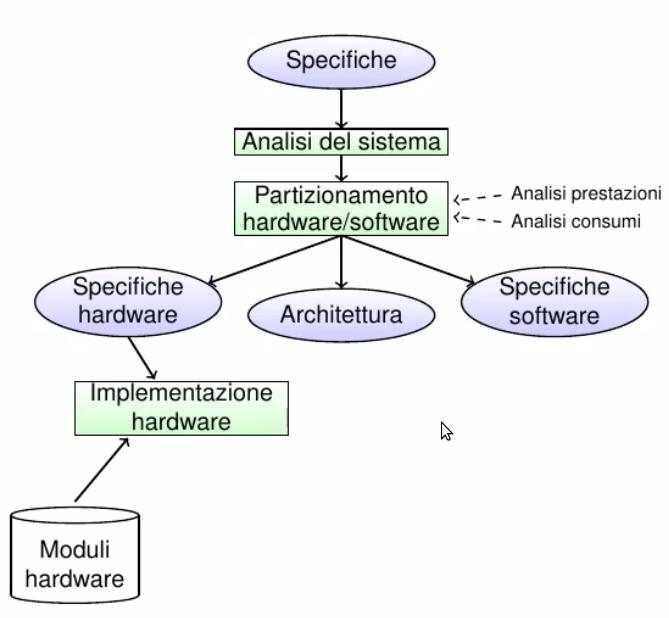
\includegraphics[scale=0.4]{immagini/image-045.jpg}
\end{figure}
C'è fase di debugging, in cui si cerca di capire cosa non funziona, quando tutto è apposto, si ha il sistema completo.\\ Sempre più spesso sistemi embedded vengono definiti con piattaforme di riferimento. Metodologia comune sono i Systems-on-Chips: la piattaforma è un dispositivo o una architettura di base che può essere facilmente modificata per realizzare nuove funzionalità o modificare quelle esistenti.\\ È utile quando il sistema embedded deve realizzare funzioni definite e regolate da standard. Processo di sviluppo è composto da due fasi: si definisce la piattaforma e poi il prodotto specifico per la piattaforma\\
\begin{figure}[!h]
\centering

\includegraphics[scale=0.4]{immagini/image-046.jpg}
\end{figure}
\subsection{Application Specific Integrated Circuit}
Si usano circuiti integrati, basata su fabbricazione planare (anni 50'): come dei fogli sottili di silicio sul quale sono ricavati i componenti elettronici, processo litografico per inglobare fogli di silicio dei circuiti integrati. Grado di miniaturizzazione si è alzato sempre, di più negli anni, circuiti integrati sono sempre più piccoli e quindi sempre più veloci (elettroni nei conduttori si spostano a velocità finita).\\ In pratica il progettista ha ampia scelta tra i circuiti integrati:
\begin{itemize}
\item COTS: componenti commerciali
\item microprocessori, micro-controllori e processori specializzati. Possono essere COTS
\item logiche programmabili
\item ASIC
\end{itemize}
\subsection{Tecnologie per ASIC}
Se un progettista deve affidare una certa funzione di un prodotto ad un circuito integrato apposito:
\begin{itemize}
\item Può usare un circuito integrato commercializzato
\item Deve progettare da solo il circuito integrato ASIC
\end{itemize}
I costi di progettazione e sviluppo di ASIC sono molto alti (anche milioni di dollari), scelta di progettare nuovo ASIC è lecita se
\begin{itemize}
\item Si richiedono dimensioni ridotte
\item SI richiedono altissime prestazioni
\item Il mercato richiede volumi molto elevati
\item Nessun COTS è adeguato
\end{itemize}
È sopratutto l'enorme costo di sviluppo di nuovi circuiti integrati che ha portato a definire piattaforme di riferimento da cui derivare nuovi prodotti.
\subsubsection{Tecnologia standard cell: soluzione}
Introdotta per semplificare la progettazione degli ASIC. Si alza il livello di astrazione con il quale si progettano i circuiti: dal transistor si passa alla cella. Una cella è un circuito digitale completo già progettato e ottimizzato da riutilizzare a piacimento.\\ Le definizioni delle celle sono raccolte in librerie commerciali. Ciascuna libreria contiene migliaia fi celle per realizzare altrettante funzioni Tutte e celle,q quando realizzate nel silicio del circuito integrato hanno la stessa altezza. Esistono programmi che calcolano il piazzamento ottimale delle celle.
\subsubsection{Tecnologia gate array}
È simile alla standard cell, nel senso che un venditore fornisce sempre una libreria di circuiti digitali. In standard cell il chip è costruito su un die di silicio puro, mentre in gate array il cihp è parzialmente fabbricato: il silicio è già organizzato in gruppi di transistor organizzati in righe regolari separate da canali di routing.\\ Una variante nota come sea of gates non possiede canali di routing, le interconnessioni sono affidate ad uno strato di metallo posto sopra ai transistor.
\subsection{Programmable Logic Device}
Chip che integrano le porte logiche e le linee di interconnessione completamente fabbricate. I chip sono programmabili, nel senso che ciascuna risorsa logica può essere configurata per svolgere una specifica funzione, ciascuna linea di interconnessione può essere collegata o meno a varie risorse logiche. Diversi gradi di programmabilità:
\begin{itemize}
\item OTP: la configurazione del chip è irreversibile ed è ottenuta applicando le tensioni elettriche più altre di quelle della normale alimentazione
\item Ri-programmabili: stabilisco dei bit all'interno di memorie per configurare il circuito. Memoria può essere volatile o persistente.
\item Ri-configurabili: posso riprogrammare anche quando il circuito è in esecuzione ed in modo selettivo.
\end{itemize}
Organizzazione delle PLD, c'è sempre alla base il  concetto di cella. Ad un estremo, la cella è costituita da una o due porte logiche, o da un multiplexer o da un flip-flop. All'altro estremo la cella può essere molto complessa, come una funzione booleana a 4 ingressi, qualche porta logica, uno o due multiplexer.\\ Vantaggio delle celle semplici è che silicio è maggiormente sfruttato, riduco rischio di sottoutilizzo di una cella.\\ Vantaggio delle celle complesse è che servono meno connessioni, perché ho meno celle. Serve cercare un compromesso, basata su cosa la PLD dovrà svolgere.
\subsubsection{Tipologie di PLD}
\begin{itemize}
\item PLA: costruito da zone di porte AND ed OR e zone di interconnessione, erano OTP
\item PAL, come i PLA ma più semplici in quanto le porte OR non sono configurabili
\item GAL: include diversi PAL, con multiplexer per retro-azionare le uscite e con flip-flop. Può inoltre essere riprogrammato.
\item CPLD: basati su celle complesse (GAL) unite da un bus di comunicazione configurabile per mezzo di una memoria EEPROM o Flash.
\item FPGA: celle complesse e interconnessioni sono distribuite regolarmente nel chip, la configurazione è in memoria generalmente volatile. Sarà utente finale a programmare il chip.\\ Sono la nuova frontiera dell'informatica: permettono di realizzare circuiti elettronici a volontà, è possibile ridefinire qualunque cosa. Ad esempio, è possibile eliminare un'istruzione macchina da microprocessore, realizzo ottimizzazione per la specifica applicazione.
\end{itemize}
\subsection{Microprocessori}
Molti sistemi embedded sono realizzati sfruttando microprocessori più o meno evoluti e specializzati. Vantaggi:
\begin{itemize}
\item Flessibilità: il software consente di avere un sistema molto più mantenibile ed estendibile
\item Se l'applicazione da realizzare è complessa, il sistema basato su microprocessore è alla fine più semplice ed economico.
\end{itemize}
Svantaggi:
\begin{itemize}
\item Le prestazioni sono peggiori, introduce ritardi rispetto ai circuiti hardware nativi dato che deve interpretare le istruzioni, consuma anche più energia, dissipazione di potenza etc...
\end{itemize}
Si possono usare microprocessori general purporse, ma anche dedicati ASP. Ancora una volta, la scelta è frutto del compromesso. Un'altra caratteristica molto importante è la forma in cui acquisire il microprocessore: COTS o IP:
\begin{itemize}
\item COTS sono chip fisicamente indipendente da integrare nel sistema
\item IP sono descrizioni a vario livello di astrazione del circuito:
\begin{itemize}
\item SOft-macro: descrizione di circuiti a livello di register transfer in linguaggio VHDL, Verilog
\item Firm-macro: a livello di gate 
\item Hard macro: a livello di layout per specifici PLD o ASIC
\end{itemize}
\end{itemize}
\subsubsection{DSP}
Altra classe di processori specifici per applicazioni sono i DSP, specializzati nell'elaborazione numerica dei segnali. Solitamente nell'elaborazione dei segnali bisogna svolgere una somma con un valore che prevede una moltiplicazione. Hanno delle operazioni MAC già integrate, quindi tipicamente eseguono l'operazione MAC in una singola istruzione\\ Sono ottimizzati per particolare flussi di esecuzione ristretti, ed hanno istruzioni per operare su più dati in parallelo.\\ Generalmente hanno insiemi very large istruction word, hanno gerarchie di memoria che distinguono tra codice e dati, quindi cambia lo spazio di indirizzamento.
\subsubsection{Network Processors}
Altra classe di processori dedicati sono i network processors, sono system-on-chip dedicati alla programmazione di rete.\\ Funzioni tipiche:
\begin{itemize}
\item Bufferizzazione di pacchetti
\item Elaborazione delle testate
\item Ricerca di indirizzi nelle tabelle
\item Calcolo di codici di controllo
\end{itemize}
Architettura di ogni NP è multi.processore, a ciascun canale è dedicato un processore.\\ Alcuni processori RISC si occupano della supervisione e dello smistamento dei pacchetti tra diversi canali. Il collegamento tra i vari processori è dato da un insieme di bus ad altissima velocità (~ 100 Gbps).\\ Generalmente RISC si programmano in C, mentre i CP si programmano in assembler o con linguaggi basati su regole lessicali di pattern recognition
\subsubsection{Microcontrollori}
Sono microprocessori che dispongono di molte periferiche ed interfacce sul circuito integrato. Sono parenteralmente adatti per le applicazioni che richiedono poca potenza di calcolo ma stretta interazione con l'hardware. es: penna USB. Microcontrollore dentro circuiti molto piccoli può fare elaborazione di protocolli come usb e dialogo con la cache. Si trova come hardware
\begin{itemize}
\item Unità logico aritmetica semplice
\item Pochi registri, uno "accumulatore"
\item Un solo bus interno, no pipeline
\item Memorie integrate persistenti tipo ROM, EEPROM di pochi KB.
\item Circuiti timer hardware
\item Piedini programmabili per I/O
\item Convertitori analogico/digitale e digitale/analogico
\item Interfacce $I^2C$, SPI, JTAG, UART, PWM.
\end{itemize}
Solitamente non possiedono interfacce sofisticare verso la memoria esterna, soprattutto per tenere basso il numero di pin del chip.
\end{document}